%%%%%%%%%%%%%%%%%%%%%%%%%%%%%%%%%%%%%%%%%%%%%%%%%%%%%%%%%%%%%%%%%%%%%%%%%%%%%%%%
%% Plantilla de memoria en LaTeX para TFG/TFM - Universidad Rey Juan Carlos
%%
%% Por Gregorio Robles <grex arroba gsyc.urjc.es>
%%     Felipe Ortega   <felipe.ortega@urjc.es>
%%     Grupo de Sistemas y Comunicaciones (GSyC)
%%     Escuela Técnica Superior de Ingenieros de Telecomunicación
%%     Universidad Rey Juan Carlos
%%
%% (Muchas ideas tomadas de Internet, colegas del GSyC, antiguos alumnos...
%%  etc. Muchas gracias a todos)
%%
%% La última versión de esta plantilla está siempre disponible en:
%%     https://github.com/glimmerphoenix/plantilla-memoria
%%
%% - Ejecución en sistema local:
%% Para obtener el documento en PDF, ejecuta en la shell:
%%   make
%%
%% A diferencia de la anterior versión, que usaba la herramienta pdfLaTeX 
%% para compilar el documento, esta nueva versión de la plantilla usa
%% XeLaTeX. Es un compilador más moderno que, entre otras mejoras, incluye
%% soporte nativo para caracteres con codificación UTF-8, traducción políglota
%% de referencias (usando Biblatex) y soporte para fuentes OTF. Esta última
%% característic permite, por ejemplo, insertar iconos de la colección 
%% Fontawesome en el texto.
%%
%% XeLaTeX viene ya incluido en todas las distribuciones modernas de LaTeX.
%%
%% - Edición y ejecución en línea: 
%% Puedes descargar y subir la plantilla a
%% Overleaf, un editor de LaTeX colaborativo en línea. Overleaf ya tiene
%% instalados todos los paquetes LaTeX y otras dependencias software para
%% que esta plantilla compile correctamente.
%%
%% IMPORTANTE: Si compilas este documento en Overleaf, recuerda cambiar
%% la configuración (botón "Menu" en la esquina superior izquierda de la interfaz)
%% y elegir la opción Compiler --> XeLaTeX. En caso contrario no funcionará.
%%
%% - Nota: las imágenes deben ir en PNG, JPG, EPS o PDF. También se pueden usar
%% imágenes en otros formatos con algunos cambios en el preámbulo del documento.

%%%%%%%%%%%%%%%%%%%%%%%%%%%%%%%%%%%%%%%%%%%%%%%%%%%%%%%%%%%%%%%%%%%%%%%%%%%%%%%%

\documentclass[a4paper, 12pt]{book}

%%-- Geometría principal (dejar activada la siguiente línea en la versión final)
\usepackage[a4paper, left=2.5cm, right=2.5cm, top=3cm, bottom=3cm]{geometry}
%%-- Activar esta línea y comentar la anterior en modo borrador, para comentarios al margen
%\usepackage[a4paper, left=2.5cm, right=2.5cm, top=3cm, bottom=3cm, marginparwidth=60pt]{geometry}

%%-- Hay que cargarlo antes que las traducciones
\usepackage{listing}                    % Listados de código

% Traducciones en XeLaTeX
\usepackage{polyglossia}
\setmainlanguage{english}
%\setmainlanguage{spanish}    % Comenta esta línea si tu memoria es en inglés

\usepackage[normalem]{ulem}  %% Para tablas
\useunder{\uline}{\ul}{}  %% Para tablas

% Traducciones particulares para español
% Caption tablas
\gappto\captionsspanish{
	\def\tablename{Table}
	\def\listingscaption{Code}
	\def\refname{Bibliography}
	\def\appendixname{Appendix}
	\def\listtablename{Table index}
	\def\listingname{Code}
	\def\listlistingname{Fragments of code index}
}

%% Tipografía y estilos
\usepackage[OT1]{fontenc}               % Keeps eulervm happy about accents encoding

% Símbolos y fuentes matemáticas elegantes: Euler virtual math fonts
% ¡Importante! Carga siempre las fuentes math AMS Euler ANTES QUE fontspec
\usepackage{amsmath}
\usepackage{amssymb}
\usepackage[OT1,euler-digits,euler-hat-accent,small]{eulervm}

% En XeLaTeX las fuentes se especifican con fontspec
\usepackage{fontspec}
\defaultfontfeatures{Scale=MatchLowercase, Ligatures=TeX}     % Default option in font config

% Fix para fuentes usadas con operadores y \mathrm
\DeclareSymbolFont{operators}{\encodingdefault}{\familydefault}{m}{n}

% Configura la fuente principal (serif): MinionPro
\setmainfont[Scale=0.96]{TeX Gyre Pagella}
% Configura la fuente sans-serif (\sffamily)
\setsansfont[Scale=MatchLowercase]{Lato}
% Configura la fuente para letra monoespaciada: Source Code Pro, escala 0.85
\setmonofont[Scale=0.85]{Source Code Pro}

%%-- Familias de fuentes específicas
%%-- Se pueden definir etiquetas para familias de fuentes personalizadas
%%-- que luego puedes emplear para cambiar el formato de una parte de texto
%%-- Ejemplo:
% \newfontfamily{\myriadprocond}{Myriad Pro Semibold Condensed.otf}

%%-- Opciones de interlineado y espacios
\linespread{1.07}                   % Aumentar interlineado para fuentes tipo Palatino
\setlength{\parskip}{\baselineskip} % Separar párrafos con línea en blanco
\usepackage[parfill]{parskip} % Mantiene alineados los párrafos

%%-- Hipervínculos
\usepackage{url}

%%-- Gráficos y tablas
\PassOptionsToPackage{
    dvipdfmx,usenames,dvipsnames,
    x11names,table}{xcolor}             % Definiciones de colores
\PassOptionsToPackage{xetex}{graphicx}

\usepackage{subfig}                     % Subfiguras
\usepackage{pgf}
\usepackage{svg}                        % Integración de imágenes en formato SVG
\usepackage{float}                      % H para posicionar figuras
\usepackage{booktabs}                   % Already loads package xcolor
\usepackage{multicol}                   % multiple column layout facilities
\usepackage{colortbl}                   % For coloured tables
\usepackage{lscape}                     % For landscape format

%%-- Bibliografía con Biblatex y Biber
% Más info:
% https://www.overleaf.com/learn/latex/Biblatex_bibliography_styles
% https://www.overleaf.com/learn/latex/biblatex_citation_styles
\usepackage[
    backend=biber,
    style=numeric,
    sorting=nty
    ]{biblatex}
\addbibresource{memoria.bib}
\DeclareFieldFormat{url}{\mkbibacro{URL}\addcolon\nobreakspace\url{#1}}
%\usepackage[nottoc, notlot, notlof, notindex]{tocbibind} %% Opciones de índice

%%-- Matemáticas e ingeniería
% El paquete units permite mostrar unidades correctamente
% Permite escribir unidades con espaciado y estilo de fuente correctos
\usepackage[ugly]{units}         
% Ejemplo de uso: $\unit[100]{m}$ or $\unitfrac[100]{m}{s}$
% Entornos matemáticos
\newtheorem{theorem}{Theorem}

% Paquetes adicionales
\usepackage{url}                        %% Gestión correcta de enlaces
\usepackage{float}                      %% H para posicionar figuras
\usepackage[nottoc, notlot, notlof, notindex]{tocbibind}    %% Opciones de índice
\usepackage{metalogo}                   %% Múltiples logos para XeLaTeX

% Fuentes especiales y glifos
\usepackage{ccicons}                % Creative Commons icons
\usepackage{metalogo}               % XeTeX logo
\usepackage{fontawesome5}           % Fontawesome 5 icons
\usepackage{adforn} 

% Blindtext
% Opciones pangram, bible, random (defecto)
\usepackage[pangram]{blindtext}
% Lorem ipsum
\usepackage{lipsum}
% Kant lipsum
\usepackage{kantlipsum}

\usepackage{fancyvrb}               % Entornos verbatim extendidos
	\fvset{fontsize=\normalsize}    % Tamaño de fuente por defecto en fancy-verbatim
	
% Configura listas (itemize, enumerate) con iconos personalizados
% Fácil reinicio de numeración con enumerate
% Info: http://ctan.org/pkg/enumitem
\usepackage[shortlabels]{enumitem}
% Usar \usageitem para configurar iconos personalizados en listas
\newcommand{\usageitem}[1]{%
	\item[%
	{\makebox[2em]{\strut\color{GSyCblue} #1}}%
	]
}

%%-- Definición de colores personalizados
% \definecolor{LightGrey}{HTML}{EEEEEE}
% \definecolor{darkred}{rgb}{0.5,0,0}     %% Refs. cruzadas
% \definecolor{darkgreen}{rgb}{0,0.5,0}   %% Citas bibliográficas
% \definecolor{darkblue}{rgb}{0,0,0.5}    %% Hiperenlaces ordinarios (también ToC)

%%-- Configuración fragmentos de código
%%-- Minted necesita Python Pygments instalado en el sistema para funcionar
%%-- En Overleaf ya está instalada esta dependencia
% \usepackage[center, labelfont=bf]{caption}
\usepackage{minted}

%%-- Se debe cargar aquí para evitar warnings
\usepackage{csquotes}                   % Para traducciones con biblatex

%%-- Glosario de términos
\usepackage[acronym]{glossaries}
\makeglossaries
\loadglsentries{glossary}

% % Definición de cabeceras del documento, usando fancyhdr
% \usepackage{fancyhdr}
% %% Configuración de cabeceras para el cuerpo principal del documento
% \pagestyle{fancy}
% \fancyhead{}
% \fancyhead[RO,LE]{\myriadprocond{\thepage}}
% \renewcommand{\chaptermark}[1]{\markboth{\chaptername\ \thechapter.\ #1}{}}
% \renewcommand{\sectionmark}[1]{\markright{\thesection.\ #1}}
% \fancyhead[RE]{\myriadprocond{\leftmark}}
% \fancyhead[LO]{\myriadprocond{\rightmark}}
% \renewcommand{\headrulewidth}{0pt}
% \setlength{\headheight}{15pt} %% Al menos 15pt para evitar warning al compilar
% \fancyfoot{}
% %% Configuración para páginas con cabecera en blanco
% \fancypagestyle{plain}{%
% \fancyhf{}% clear all header and footer fields
% \fancyhead[RO,LE]{\myriadprocond{\thepage}}
% \renewcommand{\headrulewidth}{0pt}%
% \renewcommand{\footrulewidth}{0pt}%
% }

%%-- Metadatos del doc
\title{Automatic identification of bot accounts in open-source projects}
\author{Miguel Ángel Fernández Sánchez}

%%-- Hiperenlaces, siempre se carga al final del preámbulo
\usepackage[colorlinks]{hyperref}
\hypersetup{
    pdftoolbar=true,	% Muestra barra de herramientas en Adobe Acrobat
	pdfmenubar=true,	% Muestra menú en Adobe Acrobat
	pdftitle={MSc Thesis},
	pdfauthor={Miguel Ángel Fernández},
	pdfcreator={ETSII/ETSIT, URJC},
	pdfproducer={XeLaTeX},
	pdfsubject={Topic1, Topic2, Topic3},
	pdfnewwindow=true,              %links open in new window
    colorlinks=true,                % false: boxed links; true: coloured links
    linkcolor=Firebrick4,           % enlaces internos 
    citecolor=Aquamarine4,          % enlaces a citas bibliográficas
    urlcolor=RoyalBlue3,            % hiperenlances ordinarios
    linktocpage=true                % Enlaces en núm. pág. en ToC
}

%%%---------------------------------------------------------------------------
% Comentarios en línea de revisión
% Este bloque se puede borrar cuando finalizamos el borrador

% \usepackage[colorinlistoftodos]{todonotes}
% \usepackage{verbatim}
%%%---------------------------------------------------------------------------

\begin{document}

%%-- Configuración común para todos los entornos listing
%%-- Descomentar para usar y personalizar valores
%\lstset{%
%breakatwhitespace=true,
% breaklines=true, 
% basicstyle=\footnotesize\ttfamily,
% keywordstyle=\color{blue},
% commentstyle=\color{green!40!black}, 
% language=Python} 
 

%%%%%%%%%%%%%%%%%%%%%%%%%%%%%%%%%%%%%%%%%%%%%%%%%%%%%%%%%%%%%%%%%%%%%%%%%%%%%%%%
% PORTADA

\begin{titlepage}
\begin{center}
\begin{tabular}[c]{c c}
%\includegraphics[bb=0 0 194 352, scale=0.25]{logo} &
\includegraphics[scale=1.5]{img/LogoURJC.png}
%&
%\begin{tabular}[b]{l}
%\Huge
%\textsf{UNIVERSIDAD} \\
%\Huge
%\textsf{REY JUAN CARLOS} \\
%\end{tabular}
\\
\end{tabular}

\vspace{3cm}

\Large 
MÁSTER EN DATA SCIENCE
% MASTER'S DEGREE IN DATA SCIENCE

\vspace{0.4cm}

\large
Curso Académico 2022/2023
% Academic Year 2022/2023

\vspace{0.8cm}

Trabajo Fin de Máster
% Master's Thesis

\vspace{2cm}

\LARGE AUTOMATIC IDENTIFICATION OF BOT ACCOUNTS IN OPEN-SOURCE PROJECTS
\vspace{3cm}

\large
Autor : Miguel Ángel Fernández Sánchez \\
Tutor : Dr. Felipe Ortega Soto
\end{center}
\end{titlepage}

\newpage
\mbox{}
\thispagestyle{empty} % para que no se numere esta pagina


%%%%%%%%%%%%%%%%%%%%%%%%%%%%%%%%%%%%%%%%%%%%%%%%%%%%%%%%%%%%%%%%%%%%%%%%%%%%%%%%
%%%% Para firmar
\clearpage
\pagenumbering{gobble}
\chapter*{}

\vspace{-4cm}
\begin{center}
\LARGE
\textbf{Trabajo Fin de Máster}

\vspace{1cm}
\large
Automatic Identification of Bot Accounts in Open-Source Projects.

\vspace{1cm}
\large
\textbf{Autor :} Miguel Ángel Fernández Sánchez \\
\textbf{Tutor :} Dr. Felipe Ortega Soto

\end{center}

\vspace{1cm}
La defensa del presente Trabajo Fin de Máster se realizó el día XX\qquad$\;\,$ de
\qquad\qquad\qquad\qquad \newline de 2023, siendo calificada por el siguiente tribunal:


\vspace{0.5cm}
\textbf{Presidente:}

\vspace{0.8cm}
\textbf{Secretario:}

\vspace{0.8cm}
\textbf{Vocal:}


\vspace{0.8cm}
y habiendo obtenido la siguiente calificación:

\vspace{0.8cm}
\textbf{Calificación:}


\vspace{0.8cm}
\begin{flushright}
Madrid/Móstoles/Fuenlabrada, a \qquad$\;\,$ de \qquad\qquad\qquad\qquad de 2023
\end{flushright}

%%%%%%%%%%%%%%%%%%%%%%%%%%%%%%%%%%%%%%%%%%%%%%%%%%%%%%%%%%%%%%%%%%%%%%%%%%%%%%%%
%%%% Dedicatoria

\chapter*{}
%\pagenumbering{Roman} % para comenzar la numeración de paginas en numeros romanos
\begin{flushright}
\textit{A mi familia y amigos, \\
gracias por vuestro apoyo.}
\end{flushright}

\vspace{2cm}

\begin{flushright}
\textit{To my family and friends, \\
thank you for your support.}
\end{flushright}

% \vspace{4cm}

% \begin{flushright}
% \textit{Have you ever been light years away \\
% from what you want to be? \\
% (...) \\
% I was light years away \\
% Now I've got that sunshine in my life.\\
% - "Light Years", by Jamiroquai.}
% \end{flushright}

%%%%%%%%%%%%%%%%%%%%%%%%%%%%%%%%%%%%%%%%%%%%%%%%%%%%%%%%%%%%%%%%%%%%%%%%%%%%%%%%
%%%% Agradecimientos

\chapter*{Acknowledgements}
%\addcontentsline{toc}{chapter}{Agradecimientos} % si queremos que aparezca en el índice
\markboth{Acknowledgements}{Acknowledgements} % encabezado 

% Aquí vienen los agradecimientos\ldots

% Hay más espacio para explayarse y explicar a quién agradeces su apoyo o ayuda para
% haber acabado el proyecto: familia, pareja, amigos, compañeros de clase\ldots

% También hay quien, en algunos casos, hasta agradecer a su tutor o tutores del proyecto
% la ayuda prestada\ldots

I want to thank my classmates from this Master's degree for their help and support during all the courses and through this final phase, especially Edgli, Enrique, and David. The COVID-19 pandemic arrived in our lives in the middle of our degree, so here goes a special recognition for them and the Master's professors for the extra aid and cooperation.

To my family and friends, who stood by my side all this time, bearing with me after endless promises of finishing this thesis once and for all. Your support kept me confident in the most challenging times. Specially, I want to thank my friend Quan, who also helped me solving technical issues and questions during the project.

To my tutor, Dr. Felipe Ortega, for accepting such a challenge and for the great help and guidance he provided me during this process with a lot of patience, great pieces of advice, and wise teachings. This encouraged me to keep improving and growing academically and personally throughout this project and beyond.

Last but not least, to Bitergia for supporting me in the course of this Master's degree; and also to Professor Tom Mens, Professor Alexandre Decan, and PhD student Mr. Mehdi Golzadeh from the University of Mons (Belgium); for guiding me during the early stages of this project with their generous ideas and knowledge.

%%%%%%%%%%%%%%%%%%%%%%%%%%%%%%%%%%%%%%%%%%%%%%%%%%%%%%%%%%%%%%%%%%%%%%%%%%%%%%%%
%%%% Resumen


%%%% Resumen en inglés

\chapter*{Summary}
%\addcontentsline{toc}{chapter}{Summary} % si queremos que aparezca en el índice
\markboth{SUMMARY}{SUMMARY} % encabezado

People participating in software projects (in particular, in Free, Open-Source projects) rely on many tools and platforms to support their activity on many facets, such as code review or bug management. Within this scenario, automatic accounts (also known as \emph{bot} accounts) are commonly used in software development to automate and ease repetitive or particular tasks.

Identifying these bot accounts and their activity in the projects is crucial for anyone willing to measure many aspects of the software project and the community of contributors behind it. \emph{GrimoireLab} is a tool that provides metrics about the software development process, including a component to manage the contributors' identities, with an option to mark individual profiles as bots. Nonetheless, this labelling process is entirely manual.

In this MSc thesis, a \emph{Python} tool to detect bots automatically based on their profiles' information and their activity in the project is developed. This tool can be integrated as a component inside the \emph{GrimoireLab} toolchain. To this aim, we analysed the code changes from a set of software projects from the Wikimedia Foundation, produced between January 2008 and September 2021 using GrimoireLab, labelling manually the bot accounts generating activity with the purpose of creating an input dataset to train a binary classifier to detect whether a given profile is a bot or not.

After testing different classification models using the \emph{Scikit-learn} module for \emph{Python}, the model that performed best was a ``Random Forest'' classifier, where the most relevant features were a terms score calculated based on domain-related heuristics and statistical values obtained from the individuals' activity, such as number of changes in source code or number of words and files per code change submitted to the projects.

%%%%%%%%%%%%%%%%%%%%%%%%%%%%%%%%%%%%%%%%%%%%%%%%%%%%%%%%%%%%%%%%%%%%%%%%%%%%%%%%

\chapter*{Resumen}
%\addcontentsline{toc}{chapter}{Resumen} % si queremos que aparezca en el índice
\markboth{RESUMEN}{RESUMEN} % encabezado

Las personas que participan en proyectos de \emph{software} (y en paricular en proyectos de \emph{software} libre y código abierto), se apoyan en varias herramientas y plataformas para interactuar y tratar con diferentes aspectos de estos proyectos, tales como la revisión de código o la gestión de errores o \emph{bugs}. En este contexto, las cuentas automáticas (también conocidas como cuentas \emph{bot}) se usan frecuentemente en el desarrollo de software para automatizar y simplificar ciertas tareas repetitivas o específicas.

Para cualquier persona interesada en medir ciertos aspectos de un proyecto de software y de la comunidad de personas que lo sustenta, es crucial identificar estas cuentas \emph{bot} y su actividad. \emph{GrimoireLab} es una herramienta que proporciona métricas sobre el proceso de desarrollo de \emph{software}, que incluye un componente para la gestión de los perfiles de contribuidores. Dicho componente cuenta con una opción para marcar aquellos perfiles que pertenezcan a una cuenta \emph{bot}. Sin embargo, este proceso de etiquetado es enteramente manual.

En este Trabajo de Fin de Máster se propone una herramienta desarrollada en \emph{Python} para detectar automáticamente cuentas bot, integrable como un componente dentro de \emph{GrimoireLab}, utilizando como base la información de los perfiles de los diferentes individuos y de su actividad en el proyecto analizado. Para desarrollar esta herramienta se han analizado con \emph{GrimoireLab} los cambios en el código de un conjunto de proyectos de \emph{software} de la Fundación Wikimedia, producidos entre enero de 2008 y septiembre de 2021, etiquetando manualmente aquellas cuentas \emph{bot} activas en ese periodo; con el propósito de crear un conjunto de datos (\emph{dataset}) de entrada para entrenar un clasificador binario, que detecte si un determinado perfil pertenece a una cuenta \emph{bot} o no.

Tras probar diferentes modelos de clasificación usando el módulo \emph{Scikit-learn} para \emph{Python}, el modelo que mejor resultados obtuvo fue un clasificador de tipo \emph{Random Forest}. Entre sus caraterísticas más relevantes destaca el empleo de una puntuación numérica calculada en base a heurísticos de este dominio de aplicación junto con valores estadísticos obtenidos de la actividad de los individuos, tales como el número de cambios o el numero de palabras y ficheros de cada cambio producido en los proyectos analizados.

%%%%%%%%%%%%%%%%%%%%%%%%%%%%%%%%%%%%%%%%%%%%%%%%%%%%%%%%%%%%%%%%%%%%%%%%%%%%%%%%


%%%%--------------------------------------------------------------------
% Lista de comentarios de revisión
% Se puede borrar este bloque al acabar el borrador

%\listoftodos
%\markboth{TODO LIST}{TODO LIST} % encabezado
%%%%--------------------------------------------------------------------

%%%%%%%%%%%%%%%%%%%%%%%%%%%%%%%%%%%%%%%%%%%%%%%%%%%%%%%%%%%%%%%%%%%%%%%%%%%%%%%%
%%%%%%%%%%%%%%%%%%%%%%%%%%%%%%%%%%%%%%%%%%%%%%%%%%%%%%%%%%%%%%%%%%%%%%%%%%%%%%%%
% ÍNDICES %
%%%%%%%%%%%%%%%%%%%%%%%%%%%%%%%%%%%%%%%%%%%%%%%%%%%%%%%%%%%%%%%%%%%%%%%%%%%%%%%%

% Las buenas noticias es que los índices se generan automáticamente.
% Lo único que tienes que hacer es elegir cuáles quieren que se generen,
% y comentar/descomentar esa instrucción de LaTeX.

%%-- Índice de contenidos
\tableofcontents 
\cleardoublepage
%%-- Índice de figuras
\addcontentsline{toc}{chapter}{List of Figures} % para que aparezca en el indice de contenidos
\listoffigures % indice de figuras
\cleardoublepage
%%-- Índice de tablas
\addcontentsline{toc}{chapter}{List of Tables} % para que aparezca en el indice de contenidos
\listoftables % indice de tablas
\cleardoublepage
%%-- Índice de fragmentos de código
\addcontentsline{toc}{chapter}{List of Listings} % para que aparezca en el indice de contenidos
\listoflistings

%%%%%%%%%%%%%%%%%%%%%%%%%%%%%%%%%%%%%%%%%%%%%%%%%%%%%%%%%%%%%%%%%%%%%%%%%%%%%%%%
%%%%%%%%%%%%%%%%%%%%%%%%%%%%%%%%%%%%%%%%%%%%%%%%%%%%%%%%%%%%%%%%%%%%%%%%%%%%%%%%
% INTRODUCCIÓN %
%%%%%%%%%%%%%%%%%%%%%%%%%%%%%%%%%%%%%%%%%%%%%%%%%%%%%%%%%%%%%%%%%%%%%%%%%%%%%%%%

\cleardoublepage
\chapter{Introduction}
\label{chap:intro}
\pagenumbering{arabic} % para empezar la numeración de página con números

% En este capítulo se introduce el proyecto.
% Debería tener información general sobre el mismo, dando la información sobre el contexto en el que se ha desarrollado.

% No te olvides de echarle un ojo a la página con los cinco errores de escritura más frecuentes\footnote{\url{http://www.tallerdeescritores.com/errores-de-escritura-frecuentes}}.

% Aconsejo a todo el mundo que mire y se inspire en memorias pasadas.
% Las memorias de los proyectos que he llevado yo están (casi) todas almacenadas en mi web del GSyC\footnote{\url{https://gsyc.urjc.es/~grex/pfcs/}}.

% \section{Sección}
% \label{sec:seccion}

% Esto es una sección, que es una estructura menor que un capítulo. 

% Por cierto, a veces me comentáis que no os compila por las tildes.
% Eso es un problema de codificación.
% Al guardar el archivo, guardad la codificación de ``ISO-Latin-1'' a ``UTF-8'' (o viceversa) y funcionará.

% \subsection{Estilo}
% \label{subsec:estilo}

% Recomiendo leer los consejos prácticos sobre escribir documentos científicos en \LaTeX \ de Diomidis Spinellis\footnote{\url{https://github.com/dspinellis/latex-advice}}.

% Lee sobre el uso de las comas\footnote{\url{http://narrativabreve.com/2015/02/opiniones-de-un-corrector-de-estilo-11-recetas-para-escribir-correctamente-la-coma.html}}. 
% Las comas en español no se ponen al tuntún.
% Y nunca, nunca entre el sujeto y el predicado (p.ej. en ``Yo, hago el TFG'' sobre la coma).
% La coma no debe separar el sujeto del predicado en una oración, pues se cortaría la secuencia natural del discurso.
% No se considera apropiado el uso de la llamada coma respiratoria o \emph{coma criminal}.
% Solamente se suele escribir una coma para marcar el lugar que queda cuando omitimos el verbo de una oración, pero es un caso que se da de manera muy infrecuente al escribir un texto científico (p.ej. ``El Real Madrid, campeón de Europa'').

% A continuación, viene una figura, la Figura~\ref{figura:foro_hilos}. 
% Observarás que el texto dentro de la referencia es el identificador de la figura (que se corresponden con el ``label'' dentro de la misma). 
% También habrás tomado nota de cómo se ponen las ``comillas dobles'' para que se muestren correctamente. 
% Nota que hay unas comillas de inicio (``) y otras de cierre (''), y que son diferentes.
% Volviendo a las referencias, nota que al compilar, la primera vez se crea un diccionario con las referencias, y en la segunda compilación se ``rellenan'' estas referencias. 
% Por eso hay que compilar dos veces tu memoria.
% Si no, no se crearán las referencias.

People contributing to software projects (in particular, FLOSS projects) rely on several tools to support their activity on many aspects of the project, such as source code changes, project management and coordination, software bugs or issues~\cite{dabbish-et-al-socialcoding-github12}. Data generated by such interactions can be used to extract valuable information that project managers and leaders can use to make the right decisions for the future of the project (known as data-driven decisions). Some of the most common questions while analysing an open-source project are:

\begin{itemize}
    \item How many contributors are participating?
    \item How many companies contribute to the project?
    \item How good are these participants at handling issues? 
\end{itemize}

These data are also interesting for academic purposes, as researchers and practitioners may be interested in answering a set of questions about a given project~\cite{hemmati-et-al-msr-cookbook13}.

\section{Identity problems}
\label{sec:intro-identities}

From a project management perspective, a person (generally with a manager role) needs to know their community or project. In order to get valuable insights, that person may ask two main questions:

\begin{itemize}
    \item How many unique contributors do the project have?
    \item How many different organisations are contributing to the project?
\end{itemize}

To answer these questions, we must manage contributor identities within the project.

After spotting the usage of a plethora of different tools within FLOSS projects, it is important to explain that, for interacting with each of these tools, each project contributor must be identified in some way. This could be done by creating an account or setting up a set of credentials, usually a combination of name and email. This means each contributor will end up with one or more different ``accounts'' or ``identities'' for the services the project is using.

In such a scenario, it could happen that some contributors use multiple accounts or credentials sets (from now on, we will refer to these as \textit{identities}) for the same tool or service, for instance, to differentiate the contributions made through an organisational account from those made from a personal or academic account. We name an individual as the entity representing the many identities of a contributor, its profile, and enrolment information. This problem alone entails one of the hardest challenges: how to merge identities owned by the same individual.

This is where SortingHat, a component that is part of the GrimoireLab toolset (see~\ref{ssec:GrimoireLab}), comes into play. This tool aims to ease the task of managing contributors' identities within a project or set of projects~\cite{moreno_et_al-sortinghat}. It will be described in detail in Section~\ref{sec:SortingHat}. 

\begin{figure}
 \centering
  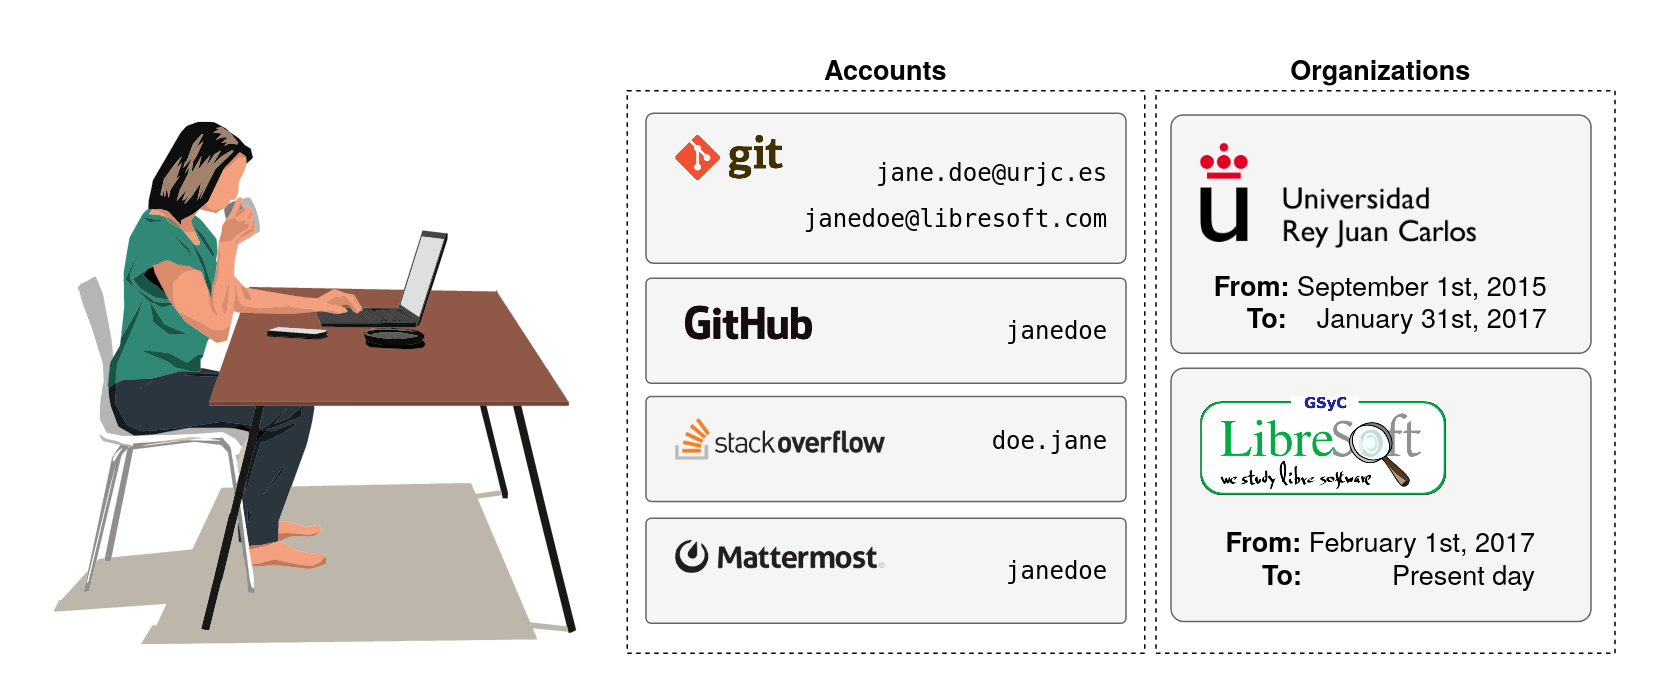
\includegraphics[width=16cm, keepaspectratio]{img/example-identity}
  \caption{A project contributor can use many accounts across different tools and platforms, besides having a number of organisational affiliations.}
  \label{fig:example-identity}
\end{figure}

\section{Automatic accounts: bots}
\label{sec:intro-bots}

It is essential to state that some interactions which occur within software development tools are not directly created by humans. Instead, they stem from an automated process set with a specific purpose and permission level to produce a specific output affecting the state of the project and its members.

This type of interaction is very common in open-source projects~\cite{erlenhov-et-al-emprirical-study-bots-oss20}, including top-level projects and communities such as GitLab\footnote{\url{https://gitlab.com/gitlab-org/gitlab}}, Wikimedia Foundation\footnote{\url{https://wikimediafoundation.org/our-work/wikimedia-projects/}} and OpenStack\footnote{\url{https://www.openstack.org/software/}}.

Some bots scan and re-post information, whereas others can also have a formal authority role associated with task evaluation. They can even play a management role combining evaluation and formal authority with interactive coordination, among other examples~\cite{hukal-et-al-bots-coordinating-oss}.

But, why is it important to identify bot accounts in open-source projects? A substantial reason is that their presence challenges any researcher or stakeholder interested in analysing the activity within a software project. Although these accounts are usually ignored in different studies, they may play an important role, as there are cases where they undertake a significant percentage of the total activity (e.g., projects where bots are responsible for accepting or rejecting 25\% of all pull requests\footnote{A request for integrating changes into a repository.})~\cite{golzadeh-mens-ground-truth-github2021}.

The number of bot accounts and their interactions depends on many factors, like:
\begin{itemize}
    \item Type and purpose of the tool or service (issue management, messaging, bug tracker, etc.).
    \item Whether this is an option provided by default by the tool or it is an \textit{ad-hoc} feature.
    \item The way these automated accounts (bots) are configured: triggered by events, periodic execution, etc.
    \item The amount of activity generated by humans or by other automatic accounts within the project.
\end{itemize}

SortingHat provides a way to mark unique identities as ``bot'' accounts by editing the identity’s profile (configuring a Boolean field named \texttt{is\_bot}). Currently, there is no automated way to identify which individuals from the whole data set could be marked as ``bots'', yet.

Up to now, this has been an entirely manual process that consumes substantial time from a person, who actively searches for suspicious identities of being bot accounts, looking at some key values such as username, email, or contribution type. This person must also double-check the original source of the data, looking for helpful extra information to verify the operator’s guesses.

\section{How this project was born}
\label{sec:intro-project-origin}

In this thesis, an approach to identify individuals from Automatic accounts (bots) is proposed, using machine learning techniques to build a classifier based on contributions produced by all identities from a given set of projects. As an additional goal, this classifier will be incorporated as a new feature in SortingHat, integrated with the original recommendation engine already implemented in it.

It is worth mentioning that this project was born within a strong research context. I had already started with this project when Prof. Tom Mens, Head of the Software Engineering Lab from the Faculty of Sciences at University of Mons (Belgium), contacted our Bitergia team to let us know about a research article regarding bot classification that they were developing at that time (September 2020). As soon I became aware of this project, I reached Prof. Tom Mens and his team to have a meeting to discuss the scope of their research and the possibility of starting a collaboration between Bitergia (the company I work for, at the time of writing this thesis) and the Software Engineering Lab from University of Mons. 

From Bitergia's point of view, this was a long-desired topic to explore, as identifying bots is a crucial part of the identity management process that our company offers to customers. For the Software Engineering Lab researchers, it was helpful to promote their new tool for bot classification BoDeGHa\footnote{\url{https://github.com/mehdigolzadeh/BoDeGHa}} (previously BoDeGa) and their goal of having better ground-truth datasets for research purposes.

%%%%%%%%%%%%%%%%%%%%%%%%%%%%%%%%%%%%%%%%%%%%%%%%%%%%%%%%%%%%%%%%%%

% %%-- Objetivos del  proyecto
% %%-- Si la sección anterior ha quedado muy extensa, se puede considerar convertir
% %%-- Las siguientes tres secciones en un capítulo independiente de la memoria

\section{Project objectives}
\label{sec:objectives}

\subsection{General objective} % título de subsección (se muestra)
\label{ssec:general-objective} % identificador de subsección (no se muestra, es para poder referenciarla)

The main objective of this project is to assess if it is possible to develop an automated or semi-automated way to classify individuals from GrimoireLab’s SortingHat into human users and bot accounts. This goal should be achieved through data obtained from each individual, using specific channels (data sources) to identify variables relevant to effectively undertaking this classification.
%  Recuerda que los objetivos siempre vienen en infinitivo.

\subsection{Specific objectives: Goals and Questions}
\label{ssec:specific-objectives}
The specific goals for this project have been defined following the ``Goal, Question, Metric'' approach. See Section~\ref{ssec:gqm-approach} for more information.
% Los objetivos específicos se pueden entender como las tareas en las que se ha desglosado el objetivo general. Y, sí, también vienen en infinitivo.

% Lo mejor suele ser utilizar una lista no numerada, como sigue:

%     \begin{itemize}
%         \item Un objetivo específico.
%         \item Otro objetivo específico.
%         \item Tercer objetivo específico.
%         \item \ldots
%     \end{itemize}

\textbf{Goal 1}: Creating an automated process to discriminate between human users and bot accounts, integrated with the GrimoireLab toolset.

\begin{itemize}
    \item \textbf{Q1.1.} How can bot accounts be separated from human users?
    \item \textbf{Q1.2.} Is the profile information from a given individual enough to classify it as human or bot?
    \item \textbf{Q1.3.} Are there differences between activity generated by humans and bots?
    \item \textbf{Q1.4.} How can this classifier be integrated into GrimoireLab’s toolchain?
\end{itemize}

\textbf{Goal 2}: Finding which channels and footprints can be used to classify a user as human or bot.

\begin{itemize}
    \item \textbf{Q2.1.} Are there any particular channels and footprints, as a combination of interactions, which can be used to classify a user as a human or bot?
    \item \textbf{Q2.2.} Can the message content (commit messages, issue texts, etc.) be used to validate this classification?
    \begin{itemize}
        \item \textbf{Q2.2.1.} Does a richer syntax give any hint about the nature of a user? 
        \item \textbf{Q2.2.2.} Can the entropy of a comment give a hint about the nature of a user?
    \end{itemize}
    \item \textbf{Q2.3.} Do activity details (such as  working hours or frequency of contributions) help with this classification?

\end{itemize}

\textbf{Goal 3}: Obtaining a curated dataset from real open-source communities with real examples of bot accounts.

\begin{itemize}
    \item \textbf{Q3.1.} Which open-source communities should be analysed?
    \item \textbf{Q3.2.} Which data sources are we taking into account?
    \begin{itemize}
        \item \textbf{Q3.2.1.} Which data should we consider form these sources?
    \end{itemize}
\end{itemize}

\section{Time planning}
\label{sec:time-planning}

% Es conveniente que incluyas una descripción de lo que te ha llevado realizar el trabajo.
% Hay gente que añade un diagrama de GANTT.
% Lo importante es que quede claro cuánto tiempo has consumido en realizar el TFG/TFM 
% (tiempo natural, p.ej., 6 meses) y a qué nivel de esfuerzo (p.ej., principalmente los 
% fines de semana).

Considering natural time, I spent, roughly, $1$ year and $7$ months working mostly 
during weekends, as I conciliated it with my full-time job. Whilst the main conversations for starting this project began in September 2020, the first stage started on March 2021. The time I spent during the first stages of the project were quite uneven, but from April 2021 I was able to keep a more regular pace until its completion on January 2023. This is the estimation of when each task was carried out and how much time was spent on it:

\begin{itemize}
\item First design of the tool, data retrieval and curation: March 2021-September 2021.
\item Designing the tool, additional work on data curation: September 2021-October 2021.
\item Building the input dataset and first experiments: October 2021-January 2022.
\item Second round of experiments: April 2022-July 2022.
\item Third round of experiments and writing the thesis: July 2022-January 2023.
\end{itemize}

%%%%%%%%%%%%%%%%%%%%%%%%%%%%%%%%%%%%%%%%%%%%%%%%%%%%%%%%%%%%%%%%%%
\section{Structure of the thesis}
\label{sec:structure}

This thesis is outlined as follows:

\begin{itemize}
    \item In this Chapter~\ref{chap:intro}, ``Introduction'', the general context and motivation is described for the problem we aim to solve. Also, the objectives for the project were already detailed in subsection~\ref{sec:objectives}, ``Project objectives''. 
    \item Next, Chapter~\ref{chap:state-art}, ``State of the Art'',  provides information about previous research work on this field and also a brief explanation of the technologies that were used during the process.
    \item The design process and architecture of the tool are detailed in Chapter~\ref{chap:design-implementation}, ``Design and Implementation'', including a breakdown of its components and a detailed analysis of the dataset obtained for the purpose of this project.
    \item In Chapter~\ref{chap:experiments}, ``Experiments and validation'', the classifiers performance and results are examined through different experiments, including the description of technical challenges encountered and how they were addressed.
    \item Wrapping up, Chapter~\ref{chap:conclusions}, ``Conclusions'' evaluates whether the set objectives were met, and includes a discussion on the limitations of the tool, lessons learned and future work.
    \item Furthermore, the Appendix~\ref{app:app-definitions}, ``Definitions'', provides additional explanations for several key terms.
\end{itemize}

There is a website dedicated to this final project\footnote{\url{https://mafesan.github.io/Memoria-TFM}}. It includes this thesis and complementary content such as the Notebooks for the exploratory data analysis and the classification experiments. In addition, the source code for this tool is available in another dedicated GitHub repository\footnote{\url{https://github.com/mafesan/2021-tfm-code}}.

% Por último, en esta sección se introduce a alto nivel la organización del resto del documento
% y qué contenidos se van a encontrar en cada capítulo.

%     \begin{itemize}
%       \item En el primer capítulo se hace una breve introducción al proyecto, se describen los objetivos del mismo y se refleja la planificación temporal.
%       \item En el siguiente capítulo se describen las tecnologías utilizadas en el desarrollo de este TFM/TFG (Capítulo~\ref{chap:tecnologias}).
%       \item En el capítulo~\ref{chap:diseño} Se describe el proceso de desarrollo
%       de la herramienta \ldots
%       \item En el capítulo~\ref{chap:experimentos} Se presentan las principales pruebas realizadas
%       para validación de la plataforma/herramienta\ldots (o resultados de los experimentos
%       efectuados).
%       \item Por último, se presentan las conclusiones del proyecto así como los trabajos futuros que podrían derivarse de éste (Capítulo~\ref{chap:conclusiones}).
%     \end{itemize}

\cleardoublepage

%%%%%%%%%%%%%%%%%%%%%%%%%%%%%%%%%%%%%%%%%%%%%%%%%%%%%%%%%%%%%%%%%%%%%%%%%%%%%%%%
%%%%%%%%%%%%%%%%%%%%%%%%%%%%%%%%%%%%%%%%%%%%%%%%%%%%%%%%%%%%%%%%%%%%%%%%%%%%%%%%
% ESTADO DEL ARTE %
%%%%%%%%%%%%%%%%%%%%%%%%%%%%%%%%%%%%%%%%%%%%%%%%%%%%%%%%%%%%%%%%%%%%%%%%%%%%%%%%

\chapter{State of the Art}               %% a.k.a "Tecnologías utilizadas"
\label{chap:state-art}

As mentioned in the Introduction chapter, this project was born within a strong research context. When I contacted Prof. Tom Mens and his team about this Master's thesis, we first exchanged ideas regarding the scope of the project and how both initiatives could complement one another. Then, they shared with me the scientific paper they were developing, aimed at detecting bots in issues and PR comments from GitHub.

A discussion followed about which research lines could be addressed for this Master's thesis. The Software Engineering Lab from University of Mons did not implement the tool, nor the underlying classifier, to detect bots based on Git commit comments or any other Git-related information. As it would be relatively easy to extend their tool to also consider Git commit comments, it was likely the classifier features that they used to distinguish bots from humans in GitHub issue and pull request comments do not work that well on Git comments. Studying, testing, and extending this behaviour was one of the main ideas they proposed to me for this Master's thesis. Likewise, this study could be extended to look at other systems and data sources. Last, but not least, it was interesting for them to learn how this classification was going to be integrated with identity merging (mainly talking about GrimoireLab's SortingHat component).

After reviewing the paper from the Software Engineering Lab at University of Mons, by Mehdi Golzadeh et al., I discovered that this text pointed to other interesting articles about the same topic, which are relevant to this Master's thesis.

\section{Research}
\label{sec:research}

In the following subsections, I summarise the two most relevant research articles on which this project is supported, and the technologies used for this project.

\begin{itemize}
    \item The first one is the article by Researcher Mehdi Golzadeh, Prof. Tom Mens et al.: \textbf{``A ground-truth dataset and classification model for detecting bots in GitHub issue and PR comments''}~\cite{golzadeh-mens-ground-truth-github2021}, on detecting bots in issue and pull request comments from OSS projects.
    
    \item The second one by Dey, B. Vacilescu et al.: \textbf{``Detecting and characterising bots that commit code''}~\cite{dey-et-al-detecting-bots}, on detecting bots contributing code in OSS\footnote{Open-Source Software.} projects.
\end{itemize}

\subsection{A ground-truth dataset and classification model for detecting bots in GitHub issue and PR comments}
\label{ssec:golzadeh}

The main goal of this paper is to propose an automated classification model to detect bots through comments submitted in GitHub issues and pull requests.

This article is divided into three large sections: First, they elaborate a ground-truth dataset of pull request and issue comments from $5K$ GitHub accounts, from which $527$ were identified as bots. Then, they propose a classification model that relies on comment-related features to classify accounts as either bot or human. Eventually, they propose an open-source tool based on the classification model to allow GitHub contributors to detect which accounts in their repositories correspond to bots.

\subsubsection{Creating the ground-truth dataset}
\label{sssec:golzadeh-dataset}

As the objective of this study is to focus on software development repositories, they need a way to identify which repositories from GitHub were created for such purpose. Hence, they rely on \textit{libraries.io}, a monitoring service indexing information for several million packages distributed through several package registries, such as PyPI, npm, etc. 

Their initial dump contains more than $3.3$ million GitHub repositories, from which they randomly select around $136K$ of them. From each of these repositories, they extract the last $100$ comments of the last $100$ issues and pull requests during $4$ days, in February 2020, using GitHub's API. They obtain over $10M$ comments from more than $837K$ contributors, and from more than $3.5M$ issues and pull requests.

After considering the size of the initial dataset, they apply some constraints to reduce it. First, they exclude users who made less than $10$ comments. This threshold comes from a previous study. Then, they extract a subset of $5K$ commenters, selected both randomly and manually, adding $438$ commenters who had been identified as bots in previous studies or contained a specific substring in their GitHub account name, such as ``bot'', ``ci'', ``cla'', ``auto'', ``logic'', ``code'', ``io'' and ``assist''.

Then, for the labelling process, they develop a web application where each commenter is presented to at least two of the four authors of the paper. Comments belonging to a certain user are displayed in batches of $20$ comments (with the option of showing more, if needed). Then, the rater can select whether the commenter is a bot or a human being. All cases that were agreed upon are included in the ground-truth dataset.

\subsubsection{Creating the classification model}
\label{sssec:golzadeh-classification}

These are the selected features to create the classification model:

\begin{enumerate}
    \item Text distance between comments.
    \begin{itemize}
        \item The main hypothesis is that bot commenters post more repetitive comments than humans do. This is why the metrics considered are text distance metrics, that are commonly used in natural language processing (NLP): the Jaccard and Levenshtein distances. The Jaccard distance~\ref{sec:jaccard-definition} aims to quantify the similarity of two texts based on their content, while the Levenshtein distance~\ref{sec:levenshtein-definition} intends to capture the structural difference by counting single-character edits.
        \item After a tokenization process, for each commenter, they compute the mean of the Jaccard and Levenshtein distances between all pairs of comments. Results show that humans get higher median values for both distances than bots. Nonetheless, there is overlapping between the values from both classes, indicating that these mean distances are not enough to properly distinguish between the two classes.
        \item Finally, a combination of both Jaccard and Levenshtein distances is used~\ref{sec:jacc-lev-comb-definition}.
    \end{itemize}
    \item Repetitive comment patterns.
        \begin{itemize}
            \item Observations suggest that bots tend to have sets of similar comments, while most comments from humans are unique, except some of them that seem to follow a pattern (mostly, short answers such as ``Thank you!'', ``\texttt{+1}'' or ``\textit{LGTM}''\footnote{ LGTM: Shorthand for ``Looks good to me''. ``\texttt{+1}'', as a common way to express agreement with something proposed in a previous comment or description.}).
            \item To capture the comment patterns, they select \textit{DBSCAN}, a density-based clustering algorithm. To capture both structural and content distance between comments, a combination of both Levenshtein and Jaccard distances is computed. For each commenter, \textit{DBSCAN} is applied to its set of comments.
            \item When the number of comment patterns (clusters) and the number of comments considered per commenter is represented, there is a clearer separation between humans and bots. The number of comment patterns for bots remained stable and low, regardless of the number of comments.
        \end{itemize}
    \item Inequality between comments in patterns
        \begin{itemize}
            \item The inequality in the number of comments in each pattern is used as an additional feature to distinguish between bots and humans by using the \textit{Gini} coefficient (a value of $0$ expresses perfect equality, while a value of $1$ expresses maximum inequality among values).
            \item Humans show a lower inequality than bots with respect to the spread of comments within patterns, confirming that humans tend to have a lower inequality than bots, a consequence of many of their patterns containing a single comment.
        \end{itemize}
    \item Number of comments and empty comments.
        \begin{itemize}
            \item This feature makes it easier to distinguish between commenters having a similar number of patterns (the ones having more comments per pattern, will more likely be a bot). 
            \item Regarding the number of empty comments, although the GitHub interface does not allow empty comments in a discussion, it does not prevent comments composed of whitespace characters. Data shows that these empty comments are mostly created by human commenters.
        \end{itemize}
\end{enumerate}

For selecting the classifier, they rely on a standard grid-search \textit{10-fold} cross-validation process to compare five families of classifiers (random forest, k-nearest neighbours, decision trees, logistic regression, and support vector machines) over the training set ($60\%$ of the ground-truth dataset) using \textit{Scikit-learn}~\ref{sssec:scikit-learn}. In addition, the class ``weight'' parameter is set to address the class imbalance problem for each supported classifier.

The $10$ subsets are created using a stratified shuffle split, to preserve the same proportion of bots and humans as in the complete training set.

The selected classifier is the ``Random forest'': using the \textit{Gini} split criterion, they get $10$ estimators (trees) and a maximum depth of $10$ for these trees. Results are available in Table~\ref{table:golzadeh-table-results}.
\smallskip

% Hemos hablado de cómo incluir figuras, pero no se ha descrito cómo incluir tablas.
% A continuación se presenta un ejemplo de tabla, la Tabla \ref{tabla:ejemplo} (fíjate 
% en cómo se introduce una referencia a la tabla).

\begin{table}[htb]  % [htb] suggests table position in page
                    % h: here; t: top; b: bottom
                    % remove any id to restrict options
 \renewcommand{\arraystretch}{1.2}  % Increase space between rows
 \begin{center}
  \begin{tabular}{  l  c  c  r  r  r }
  % \begin{tabular} { | l | c | r |} % tenemos tres colummnas, la primera alineada a la izquierda (l), la segunda al centro (c) y la tercera a la derecha (r). Se elimina el símbolo |, que indica que entre las columnas habría una línea separadora.
    \toprule    % Top table rule (horizontal) line
      & \textbf{Classified as bot} & \textbf{Classified as human} & \textbf{P} & \textbf{R} & \textbf{$F_{1}$} \\ 
      \midrule % Replace \hline for horizontal rule after table header 
    \textbf{Bot} & TP: $192$ & FN: $19$ & $0.94$ & $0.91$ & $0.92$ \\ %\hline
    \textbf{Human} & FP: $13$ & TN: $1,776$ & $0.99$ & $0.99$ & $0.99$ \\ %\hline
    \textbf{Weighted avg} &  &  & $0.98$ & $0.98$ & $0.98$ \\
    \bottomrule     % Bottom table rule (horizontal) line
  \end{tabular}
  \caption{Evaluation of the classification model using the test set.}
  \label{table:golzadeh-table-results}
 \end{center}
\end{table}

\subsubsection{BoDeGHa: an open-source tool to detect bots in GitHub repositories}
\label{sssec:golzadeh-tool}

The tool accepts as inputs the name of a GitHub repository and a GitHub API key. The output is computed in three steps:
\begin{enumerate}
    \item Download all comments from that repository through GitHub's GraphQL API, which is transformed into a list of commenters and their corresponding comments.
    \item Compute the features for the classification model: number of comments, empty comments, comment pattern, and inequality between the number of comments within patterns.
    \item Apply the pre-trained model and outputs the prediction made by the model.
\end{enumerate}

\subsubsection{Conclusions}
\label{sssec:golzadeh-conclusions}

From the $15$ bots classified as humans, most cases correspond to bots that use, convert, copy or translate text that humans initially produced. When looking at the $51$ humans classified as bots, most have unfilled issue templates, use repetitive comments such as ``Thank you'' or ``LGTM'', or post empty comments. About $85\%$ of the misclassified humans and about $75\%$ of misclassified bots are initially difficult to classify by at least one of the raters, as ``I don't know'', ``difficult'', or ``very difficult''.

They also find several examples of commenters whose behaviour and comments correspond to those of both humans and bots, that is, mixed commenters using their GitHub accounts belonging to humans allowing automatic tools to make use of the account for specific tasks. These cases represent the $1.5\%$ ($78$ commenters out of $5,082$), and they exclude them from the ground-truth dataset, as they can not decide whether these commenters should be classified as bots or as humans. The mixed commenters are exposed to test how the model behaved with these cases, resulting in $29$ being classified as bots ($37.2\%$) and $49$ as humans ($62.8\%$). 

Although other articles, such as the one from Dey et al. (explained in the following subsection), proposed approaches for identifying bot accounts based on their commit messages or their author information, such as checking the presence of the string ``bot'' in the account name or the committer name, it lead to numerous both false positives and false negatives.

\subsection{Detecting and characterising bots that commit code}
\label{ssec:dey}

The main goal of this article is to find an automated way of identifying bots (and their contributions) that commit code in open-source projects and characterise them according to their activity.

To do so, they propose a systematic approach named \textbf{BIMAN} (\emph{Bot Identification by commit Message, commit Association and author Name}) to detect bots considering different aspects of the commits made by an author:
\begin{enumerate}
    \item Commit Message: Identify if commit messages are being generated from templates.
    \item Commit Association: Predict if an author is a bot using a random forest model, using features related to the information from the commits as predictors.
    \item Author Name: Match the author's name and email to common bot patterns.
\end{enumerate}

This method is applied to the \emph{World of Code} dataset~\cite{mockus-woc}, obtaining a subset of the data, gathering information about $461$ bots detected by this approach and manually verifying as bots, each with more than $1,000$ commits.

Their method to extract information about the authors consists of these steps: First, obtaining a list of all authors from the \emph{World of Code} dataset\footnote{The author's IDs are represented by a combination of name and email address.}. 
Second, identifying all commits from the authors. And third, extracting the list of files modified by a commit, the list of projects the commit is associated with, and the commit content for each commit for every author.

That being said, \textbf{BIMAN} (the proposed technique for detecting bots) comprises three methods, which are detailed in the following subsections. This dataset is also used to characterise the bots based on their patterns, such as the type of files modified and time distribution, to analyse their work, and the programming languages they use.

\subsubsection{Identifying bots by name (BIN)}
\label{sssec:dey-bin}

After inspecting the dataset, regular expressions are used to identify if an author is a bot by checking if the author's name or the email contains the substring \texttt{bot}. These expressions have restrictions, like searching for the string preceded and followed by non-alpha characters (to avoid false positives, such as names like ``Abbot'') and excluding from this search the email domain.

The initial assumption is that bots are very active and produce a significantly greater number of commits than humans. However, the observations show that the number of commits between humans and bots is not quite different. Among the reasons behind this statement, one is that given an author ID consisting of a name-email combination, slight variations in this combination lead to consider some cases as different authors when they are not. Besides, bots might have been implemented as an experiment or as part of a course and never used afterwards. Another reason can be that some bots were designed for a project, but in the end, they were never fully adopted.

\subsubsection{Detecting bots by commit messages (BIM)}
\label{sssec:dey-bim}

The primary assumption is considering that bots use template messages as the starting point for the commit message. Thus, the goal is detecting if the commit message came from a template. Although humans can also generate commit messages with similar patterns, the hypothesis is that the variability of content within messages generated by bots is lower than the messages coming from humans.

The \textbf{BIM} approach uses a document template score algorithm, which compares document pairs and uses a similarity measure to group documents. A group represents documents suspicious of conforming to a similar base document. Each group has a single template document assigned to it, and this document is used for comparisons. A new group is created when the similarity of a document does not reach the threshold with any other template document for that group. After this, documents are compared, and a score is calculated based on the ratio of the number of template documents and the number of documents. 

\subsubsection{Detecting bots by files changed and projects associated with commits (BICA)}
\label{sssec:dey-bica}

Twenty metrics are used as a starting point, using the files changed by each commit, the projects that the commit is associated with, and the timestamp and timezone of the commits.

The random forest model performs better than other approaches for predicting whether an author is a bot using the numerical features. Out of the $20$ variables, only six features are retained as predictors (see Table~\ref{table:dey-table-predictors}).

\begin{table}[htb]
\renewcommand{\arraystretch}{1.2}
 \begin{center}
  \begin{tabular}{   p{5cm}   % p{Xcm} paragraph mode, row length
    >{\raggedright\arraybackslash} p{10cm} }  
    % >{\raggedright\arraybackslash} avoids word splitting between row lines
    \toprule
    %\rowcolor[HTML]{C0C0C0}  % Do not mix colors w/ horizontal rules
    \textbf{Variable name} & \textbf{Variable description}\\ 
    \midrule
    Tot.FilesChanged & Number of files changed by author across commits  \\ %\hline
    Uniq.File.Exten & Num. of unique file extensions in all the author's commits \\ %\hline
    Std.File.pCommit & Std. dev. of number of files per commit \\ %\hline
    Avg.File.pCommit & Mean number of files per commit \\ %\hline
    Tot.uniq.Projects & Num. of unique projects associated with commits\\ %\hline
    Median.Project.pCommit & Median num. of projects associated with commits\\
    \bottomrule
  \end{tabular}
  \caption{Predictors used in the random forest model for BICA.}
  \label{table:dey-table-predictors}
 \end{center}
\end{table}


\subsubsection{Ensemble model}
\label{sssec:dey-ensemble}

The ensemble model is implemented as another random forest model and combine the outputs of the three methods explained so far (\textbf{BIN}, \textbf{BIM} and \textbf{BICA}) as predictors to make a final decision on whether an author is a bot or not.

Since the golden dataset is generated using the BIN method, the authors do not use it for training the ensemble model. Instead, they create a new training dataset partly consisting of $67$ bots from which $57$ author IDs are associated with eight bots and ten author IDs are linked to three other known bots that are not in the golden dataset. Furthermore, $67$ human authors are included via random selection and manual validation. 

The output from \textbf{BIN} is a binary value stating if the author ID matches the regular expressions detailed before; the output from \textbf{BIM} is a score, with higher values corresponding to a higher probability of the author being a bot; and the output from \textbf{BICA} is the probability for an author of being a bot.

\begin{figure}
 \centering
  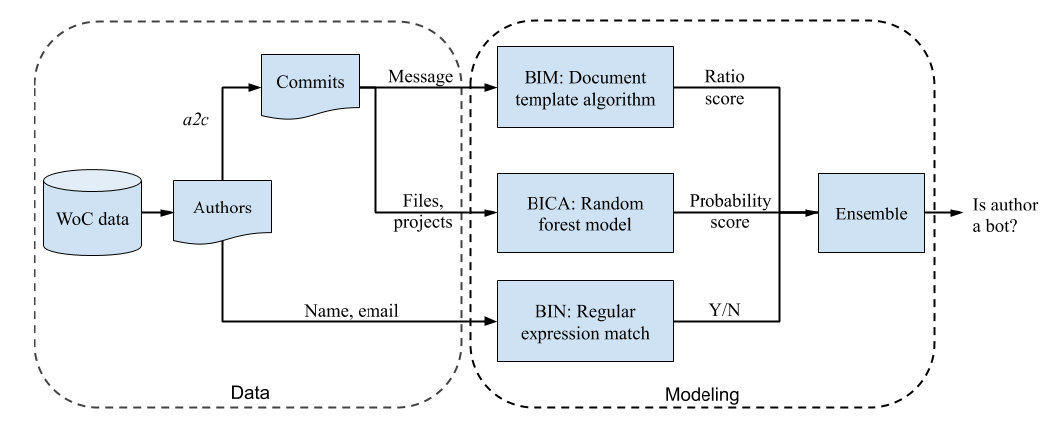
\includegraphics[width=15cm, keepaspectratio]{img/BIMAN-workflow.png}
  \caption{BIMAN workflow: Scores from each method are used by an ensemble model that classifies the given author as a bot or not a bot (taken from the original paper).}
  \label{fig:biman-workflow}
\end{figure}

\subsubsection{BIMAN results}
\label{sssec:dey-results-biman}

\textbf{BIMAN} identifies $58$ ($87\%$) out of $67$ author IDs as bots, and $6$ out of $9$ other IDs could be identified as not actually being a bot via manual investigation, they are either
spoofing the name or simply using the same name. 

\textbf{BIN performance}: during creation of the golden dataset, BIN obtains a precision close to $99\%$, which indicates that any author considered to be a bot using this method has a very high probability of being a bot. In general, humans do not try to disguise themselves as bots. The recall measure is not high, because BIN misses many cases where the bots do not explicitly have the substring ``\texttt{bot}'' in their name.

\textbf{BIM performance}: the document template score algorithm solely relies on the commit messages. The AUC-ROC value using the ratio values as predicted probabilities is $0.7$. Some details about the classification output:
\begin{itemize}
	\item \textbf{True Positive}: The cases where this model can correctly identify
bots are cases where the bots actually use templates or repeat the same commit message. 
    \item \textbf{False Negative}: The cases where this model cannot correctly identify bots are mostly cases where the bots review code added by humans and create a commit message that adds a few words with the commit message written by a human.
    \item \textbf{True Negative}: The human authors correctly identified have some variation in the text, with the usual descriptions of change.
    \item \textbf{False Positive}: Humans who are misclassified as bots usually have short commit messages that are not descriptive, and they reuse the same commit message multiple times.
\end{itemize}

\textbf{BICA performance}: The golden dataset generated using the \textbf{BIN} method is used for training the model and testing its performance. $70\%$ of the data, randomly selected, is used for training the model and the rest $30\%$ is used for testing. This procedure is repeated $100$ times with different random seeds. The model shows good performance, with an AUC-ROC value of $0.89$.

\textbf{Ensemble model performance}: The dataset used for training and testing the performance of this model has only $134$ observations, because of reasons described in Section~\ref{sssec:dey-ensemble}. $80\%$ of the data are used for training, and $20\%$ for testing. The process is repeated $100$ times with different random seeds. The value of the AUC-ROC measure varies between $0.89$ and $0.95$, with a median of $0.90$.

\subsubsection{Conclusions}
\label{sssec:dey-conclusions}

After studying the results, the authors conclude that a significant portion of authors can be identified as bots using the proposed method.

Among the limitations for this approach, they mention the lack of a golden dataset and the lack of a ground truth to validate this dataset against. Like in the previous article, another threat is that a number of developers use automated scripts to handle some of their works, which uses their Git credentials while making commits.

Moreover, they mention that \textbf{BIM}’s performance varies according to the language of the commit messages (e.g., Spanish and Chinese), and it does not support multilingual sets of commit messages.

They do not address the problem of multiple IDs belonging to the same author, so this is planned as future work to extend the \textbf{BIMAN} method.

\section{Technologies}
\label{sec:Technologies}

\subsection{GQM approach}
\label{ssec:gqm-approach}

The ``Goal Question Metric'' (GQM) approach~\cite{Basili94-gqm} is based upon the assumption that for measuring purposefully, first the goals must be specified for the project, then those goals must be traced to the data that are intended to define these goals operationally, and finally to provide a framework for interpreting the data with respect to the stated goals.

This approach helps to define the metrics that matter in each case, avoiding frequent bad practices. For example, people tend to use or define a set of metrics without having a clear idea about the specific goals they pursue. This usually leads to a ``bottom-up'' approach: besides having metrics misaligned with the project or business goals, the set of metrics may also be biased by the current technology applied to obtain these metrics.

The lack of a well-defined strategy also hinders practitioners from understanding which metrics are important and why. By using a ``top-down'' approach (first goals, then metrics), it becomes easier to materialise a targeted set of questions for the current situation and then check which metrics could be useful in the future or not, or how these metrics can help to reach the different goals by answering the questions that were raised.

\begin{figure}
 \centering
  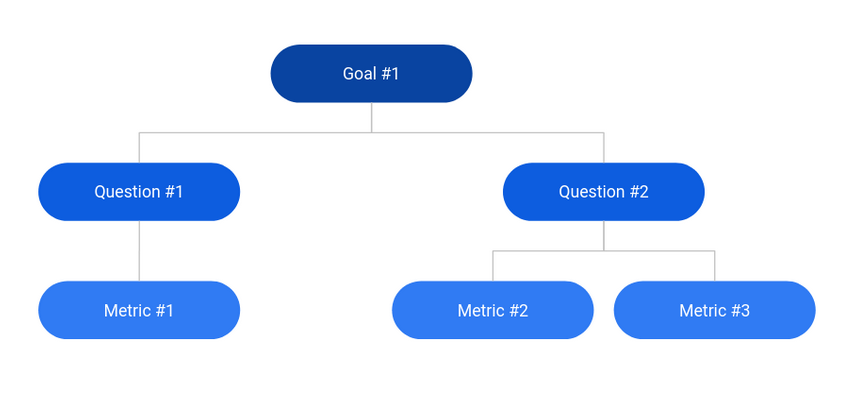
\includegraphics[width=12cm, keepaspectratio]{img/example-gqm-schema}
  \caption{Example: Goal, Question, Metric approach hierarchy.}
  \label{fig:example-gqm-schema}
\end{figure}

\subsection{GrimoireLab}
\label{ssec:GrimoireLab}
GrimoireLab~\footnote{\url{https://chaoss.github.io/grimoirelab/}} is a free, open-source toolset for producing software development analytics.

This toolset provides a whole platform that supports automatic and incremental data gathering from many tools (data sources or \emph{backends}) related to open-source development (source code management, issue tracking systems, messaging tools, mailing lists, etc.).

Data obtained from these tools is stored in JSON documents following a uniform format, no matter the source. These JSON documents are stored in ElasticSearch and, then, undergo a data enrichment process which adds additional information such time calculations (delays, duration), contributors' affiliation, and more.
Once the data have been augmented, they can be consumed by visualisation tools and also directly using the ElasticSearch API. GrimoireLab toolset comes with a tool named ``Kibiter'' which is a \emph{fork} of Elastic's Kibana. A set of predefined dashboards and visualisations are included for each data source.  

GrimoireLab is part of CHAOSS~\footnote{\url{https://chaoss.community/about-chaoss/}}, a project sponsored by The Linux Foundation. It is mainly developed by the Spanish company Bitergia, and represents an evolution of the work done over more than $10$ years in Bitergia and the LibreSoft research group at Rey Juan Carlos University.

\subsection{SortingHat}
\label{sec:SortingHat}

SortingHat is the GrimoireLab component for identity management. It provides more than 20 commands to manipulate identities, including support for:

\begin{enumerate}[label=\roman*)]
    \item identity merging based on email addresses, usernames, and full names found on many tools used in software development;
    \item  enrolling members to organisations for a given time span, marking identities as automatic accounts (bots);
    \item gender assessment, among other features~\cite{moreno_et_al-sortinghat};
\end{enumerate}

This tool maintains a relational database with identities and related information extracted from different tools used in software development. An identity is a tuple composed of a name, email, username, and the source's name from where it was extracted. Tuples are converted to unique identifiers (i.e., uuid), which provide a quick mean to compare identities among each other. By default, SortingHat considers all identities as unique ones. Heuristics take care to automatically merge identities based on perfect matches on \((i)\) uuids, \((ii)\) name, \((iii)\) email, or \((iv)\) username.

In case of a positive match, an identity is randomly selected as the unique one, and the other identities are linked to it.

Currently, SortingHat is evolving into a service-based application implementing a \emph{GraphQL API} in \emph{Python}.

\subsection{Python}
\label{ssec:python}

\textbf{Python}~\footnote{\url{https://www.python.org/}} is an interpreted, object-oriented, high-level, open-source
programming language for general-purpose programming created by Guido van Rossum in 1991~\cite{van2007python}. Nowadays, the most
recent version is $3.11.2$, from February 2023. Its design is focused on code readability and clear syntax, making
it possible to program using fewer lines of code compared to other programming languages such as \emph{C++} or \emph{Ada}.

\emph{Python} features a large standard library, which includes many tasks from text pattern matching to network
scripting, in addition to a vast collection of third-party application libraries.
Other remarkable features are portability, as \emph{Python} interpreters are available for many operating systems;
and the component integration, as \emph{Python} scripts can easily communicate with other parts of an application or code,
like \emph{C++} libraries, \emph{MySQL} databases, etc.

In this case, we focus on libraries oriented towards data science. Next, we describe several important libraries utilised in this project.

\subsubsection{NumPy and Pandas}
\label{sssec:numpy-pandas}

\textbf{NumPy}~\footnote{\url{https://numpy.org/}} is an open-source project aiming to enable numerical computing with Python. It was created in 2005, building on the early work of the Numeric and Numarray libraries. 

NumPy has become the fundamental package for scientific computing in Python. It is a Python library that provides a multidimensional array object, various derived objects (such as masked arrays and matrices), and an assortment of routines for fast operations on arrays, including mathematical, logical, shape manipulation, sorting, selecting, I/O, discrete Fourier transforms, basic linear algebra, basic statistical operations, random simulation and much more.

\textbf{Pandas}~\footnote{\url{https://pandas.pydata.org/}} is an open-source data analysis and manipulation tool, built on top of the Python programming language. This library was developed as an extension of NumPy, and it offers efficient data structures (such as \emph{Dataframes}) and operations to handle with numeric tables and time series.

\subsubsection{Matplotlib}
\label{sssec:matplotlib}

Matplotlib~\footnote{\url{https://matplotlib.org/}} is a plotting library for the Python programming language and its numerical mathematics extension NumPy. It provides an object-oriented API for embedding plots into applications using general-purpose GUI toolkits.

\subsubsection{Jupyter Notebooks}
\label{sssec:jupyter-notebooks}

Jupyter Notebook\footnote{\url{https://jupyter-notebook.readthedocs.io/en/stable/}} (formerly IPython Notebooks) is a web-based interactive computational environment for creating notebook documents.

A Jupyter Notebook document is a browser-based interactive, simple programming environment containing an ordered list of input/output cells which can contain code, text in \emph{Markdown} format, mathematics, plots and rich media. Underneath the interface, a notebook is a JSON document, following a versioned schema, usually ending with the \texttt{.ipynb} extension.

Jupyter notebooks are built upon a number of popular open-source libraries, such as IPython~\footnote{\url{https://ipython.readthedocs.io/en/stable/}}.

\subsubsection{Imbalanced-learn}
\label{sssec:imblearn}

Imbalanced-learn\footnote{\url{https://imbalanced-learn.org/stable/index.html}} (imported as Python module as \texttt{imblearn}) is an open-source, MIT-licensed library relying on scikit-learn (imported as sklearn) and provides tools when dealing with classification with imbalanced classes.

\subsubsection{Scikit-learn}
\label{sssec:scikit-learn}

Scikit-learn\footnote{\url{https://scikit-learn.org}} is largely written in Python, and uses NumPy extensively for high-performance linear algebra and array operations. Furthermore, some core algorithms are written in \emph{Cython} (a super-set of the Python language that additionally supports calling \emph{C} functions) to improve performance.

The classification models proposed and tested for this project are based on this library. 

\subsubsection{XGBoost}
\label{sssec:state-art-xgboost}

XGBoost\footnote{\url{https://github.com/dmlc/xgboost}} (from \textit{eXtreme Gradient Boosting}) is an open-source, optimised distributed gradient boosting library designed to be highly efficient, flexible, and portable. It implements machine learning algorithms under the Gradient Boosting framework. XGBoost provides a parallel tree boosting (also known as GBDT, GBM) that solves many data science problems in a fast and accurate way.


\subsection{Git}
\label{ssec:git}

\textbf{Git} is an open-source Version Control System (\emph{VCS}), originally developed in 2005 by Linus Torvalds~\cite{somasundaram2013git}.
Like any other \emph{VCS}, \emph{git} is a system that records changes to a file or set of files over time
so that you can recall specific versions later. According to the last surveys, it is by far the most used \emph{VCS} in the
world\footnote{\url{https://insights.stackoverflow.com/survey/2021}}.

\emph{Git} thinks of its data more like a series of snapshots of a miniature file system (See Figure~\ref{fig:info-git}).
Every time you commit or save the state of your project, it basically takes a picture of what all
your files look like at that moment and stores a reference to that snapshot. To be efficient, if files have not changed,
\emph{git} does not store the file again, just a link to the previous identical file it has already stored.
All this information is stored in a key-value system as \emph{git} objects, with a unique identity for each of them.

\begin{figure}
  \centering
  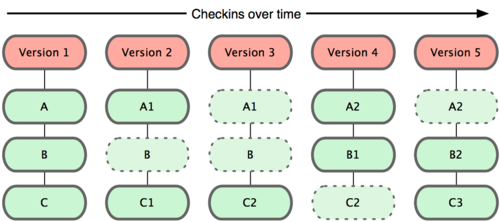
\includegraphics[width=12cm, keepaspectratio]{img/snapshots-git}
  \caption{How \emph{git} structures its information internally~\cite{progit2014book}.}
  \label{fig:info-git}
\end{figure}

% Puedes citar libros, como el de Bonabeau et al., sobre procesos estigmérgicos~\cite{bonabeau:_swarm}. 
% Me encantan los procesos estigmérgicos.
% Deberías leer más sobre ellos.
% Pero quizás no ahora, que tenemos que terminar la memoria para sacarnos por fin el título.
% Nota que el \~ \ añade un espacio en blanco, pero no deja que exista un salto de línea. 
% Imprescindible ponerlo para las citas.

% Citar es importantísimo en textos científico-técnicos. 
% Porque no partimos de cero.
% Es más, partir de cero es de tontos; lo suyo es aprovecharse de lo ya existente para construir encima y hacer cosas más sofisticadas.
% ¿Dónde puedo encontrar textos científicos que referenciar?
% Un buen sitio es Google Scholar\footnote{\url{http://scholar.google.com}}.
% Por ejemplo, si buscas por ``stigmergy libre software'' para encontrar trabajo sobre software libre y el concepto de \emph{estigmergia} (¿te he comentado que me gusta el concepto de estigmergia ya?), encontrarás un artículo que escribí hace tiempo cuyo título es ``Self-organized development in libre software: a model based on the stigmergy concept''.
% Si pulsas sobre las comillas dobles (entre la estrella y el ``citado por ...'', justo debajo del extracto del resumen del artículo, te saldrá una ventana emergente con cómo citar.
% Abajo a la derecha, aparece un enlace BibTeX.
% Púlsalo y encontrarás la referencia en formato BibTeX, tal que así:

% \clearpage
% {\footnotesize
% \begin{minted}{bibtex}
% @inproceedings{robles2005self,
%   title={Self-organized development in libre software:
%          a model based on the stigmergy concept},
%   author={Robles, Gregorio and Merelo, Juan Juli\'an 
%           and Gonz\'alez-Barahona, Jes\'us M.},
%   booktitle={ProSim'05},
%   year={2005}
% }
% \end{minted}
% }

% Copia el texto en BibTeX y pégalo en el fichero \texttt{memoria.bib}, que es donde están las referencias bibliográficas.
% Para incluir la referencia en el texto de la memoria, deberás citarlo, como hemos hecho antes con~\cite{bonabeau:_swarm}, lo que pasa es que en vez de el identificador de la cita anterior (bonabeau:\_swarm), tendrás que poner el nuevo (robles2005self).
% Compila el fichero \texttt{memoria.tex} (\texttt{pdflatex memoria.tex}), añade la bibliografía (\texttt{bibtex memoria.aux}) y vuelve a compilar \texttt{memoria.tex} (\texttt{pdflatex memoria.tex})\ldots y \emph{voilà} ¡tenemos una nueva cita~\cite{robles2005self}!

% También existe la posibilidad de poner notas al pie de página, por ejemplo, una para indicarte que visite la página del GSyC\footnote{\url{http://gsyc.es}}.

%%-- El comando \gls{} permite incluir términos en el glosario, para luego reunirlos todos
%%-- en una tabla al comienzo o al final del documento, junto con sus definiciones.

% PyCharm es un \gls{ide} dedicado concretamente a la programación en Python y desarrollado por la compañía checa JetBrains.


\cleardoublepage

%%%%%%%%%%%%%%%%%%%%%%%%%%%%%%%%%%%%%%%%%%%%%%%%%%%%%%%%%%%%%%%%%%%%%%%%%%%%%%%%
%%%%%%%%%%%%%%%%%%%%%%%%%%%%%%%%%%%%%%%%%%%%%%%%%%%%%%%%%%%%%%%%%%%%%%%%%%%%%%%%
% DISEÑO E IMPLEMENTACIÓN %
%%%%%%%%%%%%%%%%%%%%%%%%%%%%%%%%%%%%%%%%%%%%%%%%%%%%%%%%%%%%%%%%%%%%%%%%%%%%%%%%

\chapter{Design and implementation}
\label{chap:design-implementation}

The proposed tool for this project, \emph{Revelio}, aims to provide a report with the results of an automatic classification to discriminate bot accounts from the rest, over the available information from individuals in a given GrimoireLab instance.

% Aquí viene todo lo que has hecho tú (tecnológicamente). 
% Puedes entrar hasta el detalle. 
% Es la parte más importante de la memoria, porque describe lo que has hecho tú.
% Eso sí, normalmente aconsejo no poner código, sino diagramas.

\section{General architecture} 
\label{sec:architecture}

\begin{figure}
  \centering
  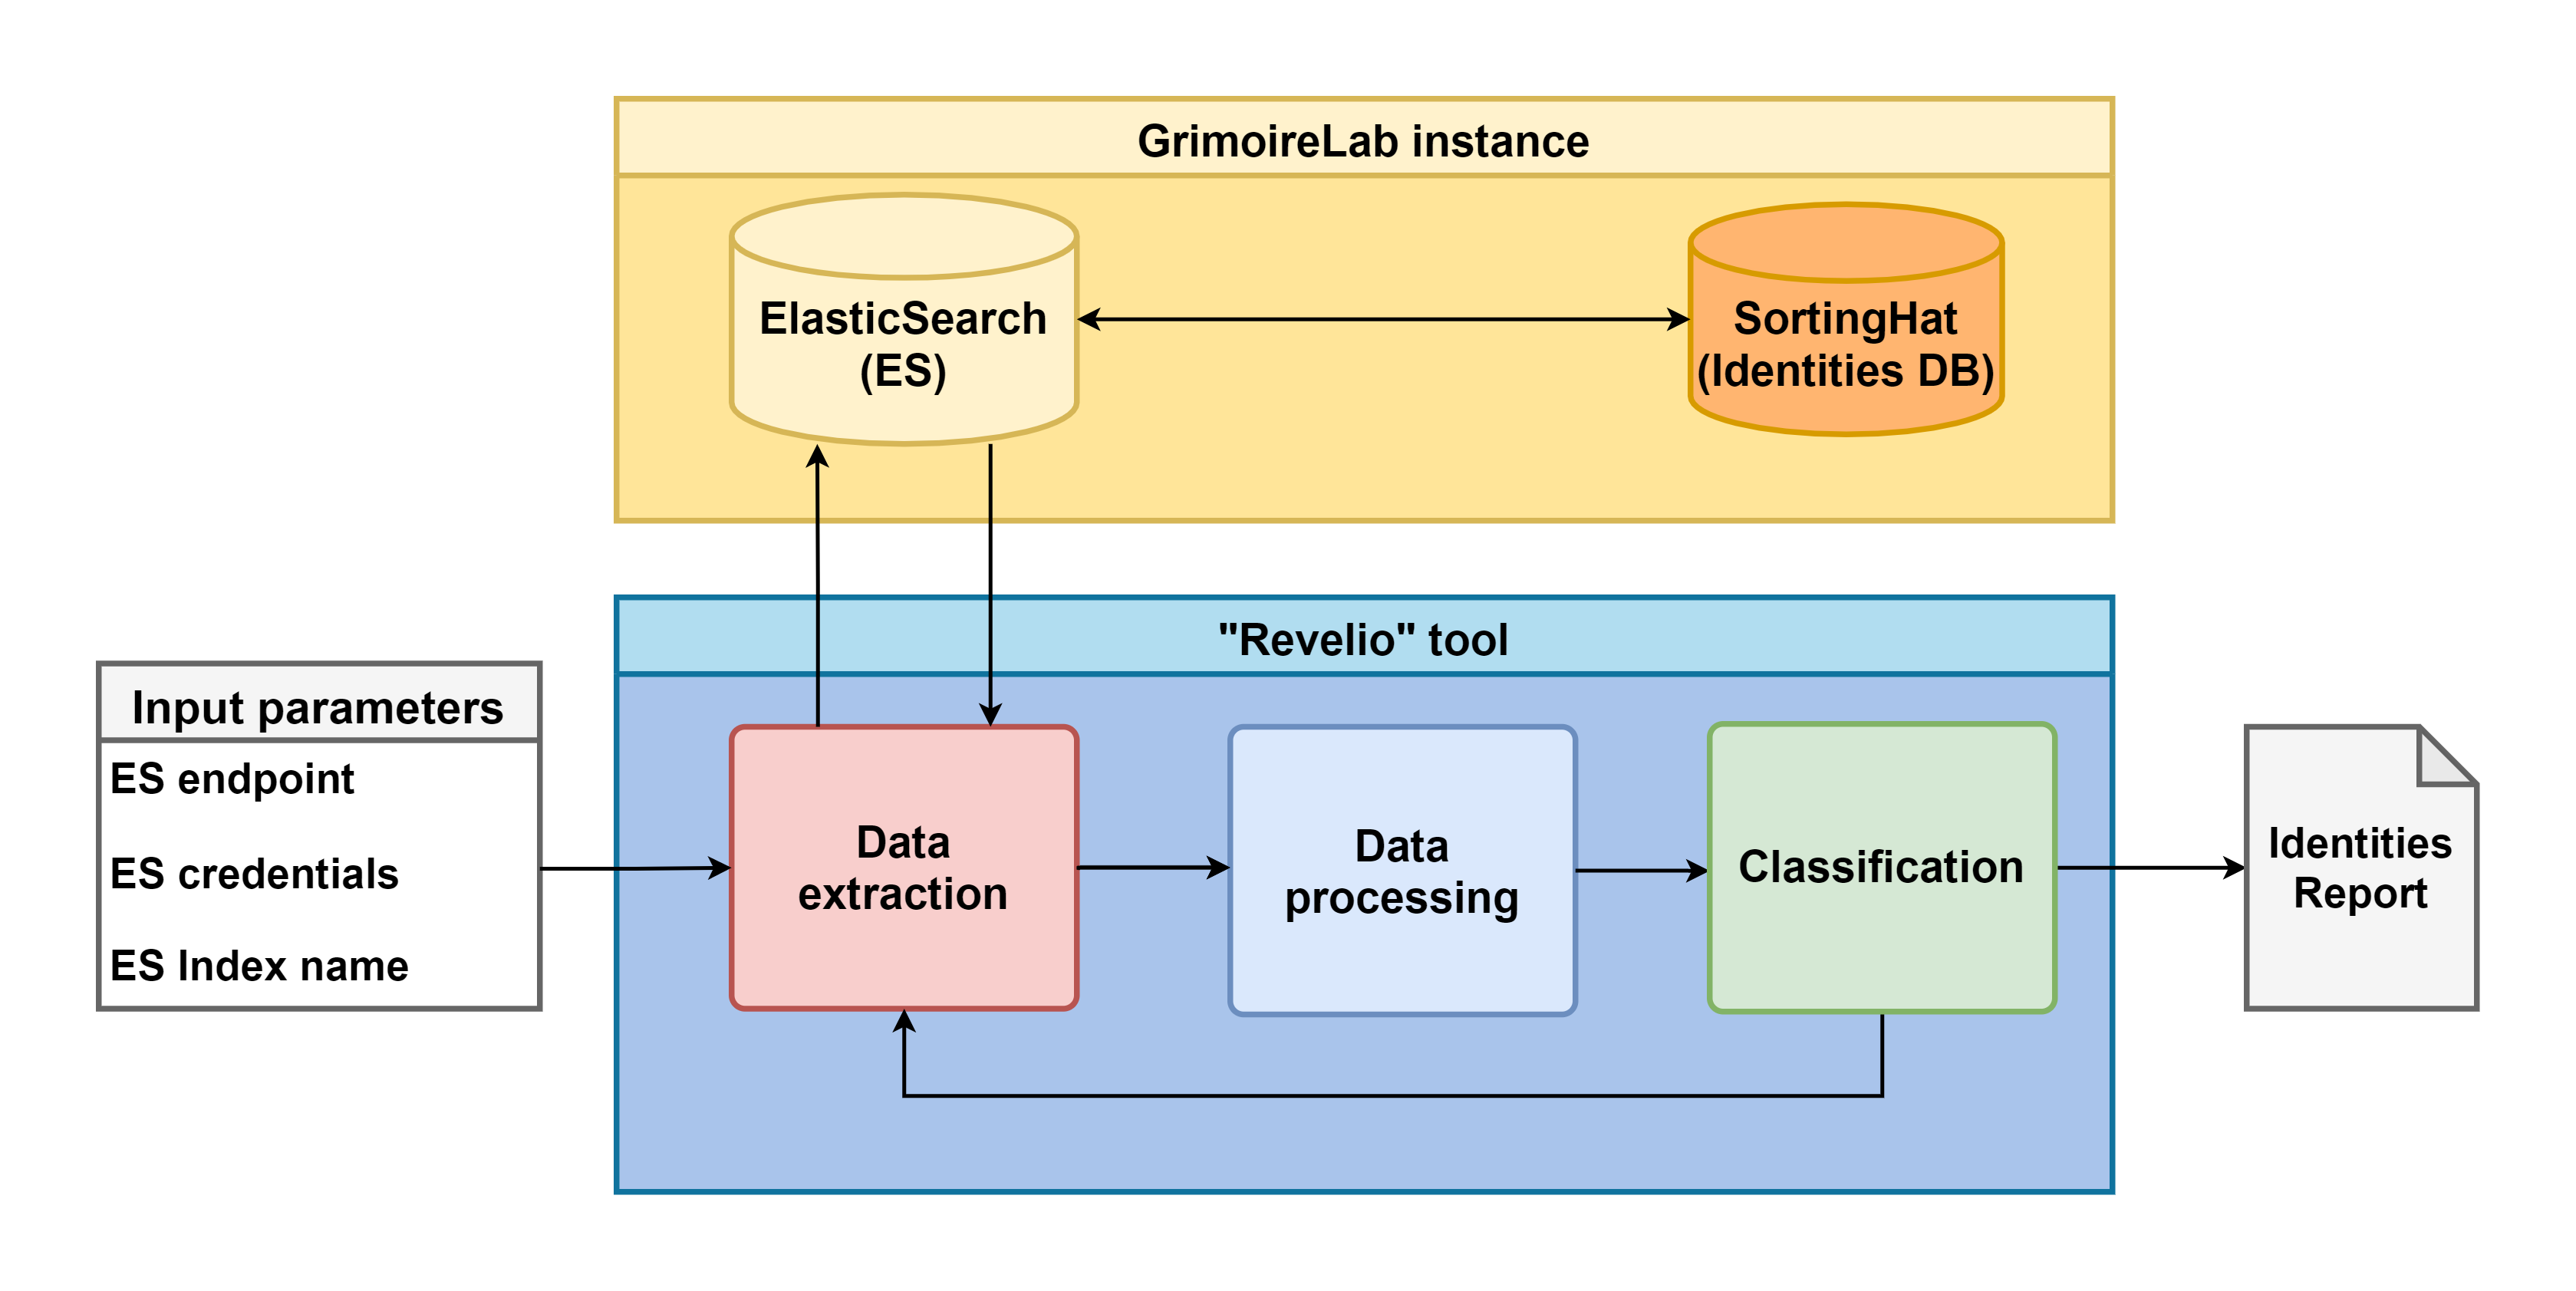
\includegraphics[width=17cm, keepaspectratio]{img/general-architecture-revelio.png}
  \caption{General architecture of the \emph{Revelio} tool.}
  \label{fig:general-arch-revelio}
\end{figure}

\emph{Revelio} is a tool which has been designed to be composed by different modules (see Figure~\ref{fig:general-arch-revelio}), to ease its adaptability to future updates and extensions. Each
of these modules consist on one or more scripts.

As a general description, the tool requires a running GrimoireLab instance to execute. This GrimoireLab instance would contain data from many endpoints stored in an ElasticSearch instance, together with a relational database containing identity information.

With the GrimoireLab instance in place, \emph{Revelio} accepts three main input parameters:
\begin{itemize}
    \item The URL or the IP address of the ElasticSearch instance.
    \item The credentials to access ElasticSearch and SortingHat.
    \item The index name from ElasticSearch, containing the GrimoireLab-formatted data.
\end{itemize}

With these input parameters, the tool executes the following steps:

\begin{enumerate}
    \item \textbf{Data extraction}: \emph{Revelio} extracts the data
    per individual from the selected index querying the
    ElasticSearch instance.
    \item \textbf{Data processing}: The extracted data is analysed
    and processed, creating the datasets for the classification
    phase.
    \item \textbf{Classification}: In this phase, the classification
    models are defined and adjusted. The output of this chain is a
    report containing the results of the classification: An
    attribute \texttt{is\_bot} for each individual, and
    another attribute for the accuracy of the result, \texttt{accuracy}.
\end{enumerate}

In the following sections, the structure and the implementation of the tool are explained. Each main phase from the general structure is more detailed in the diagram from Figure~\ref{fig:process-arch}: keeping the colour code from Figure~\ref{fig:general-arch-revelio}, this diagram shows the sub-modules from each main part of the tool and the execution flow detailed in the sections and subsections below.

\begin{figure}
  \centering
  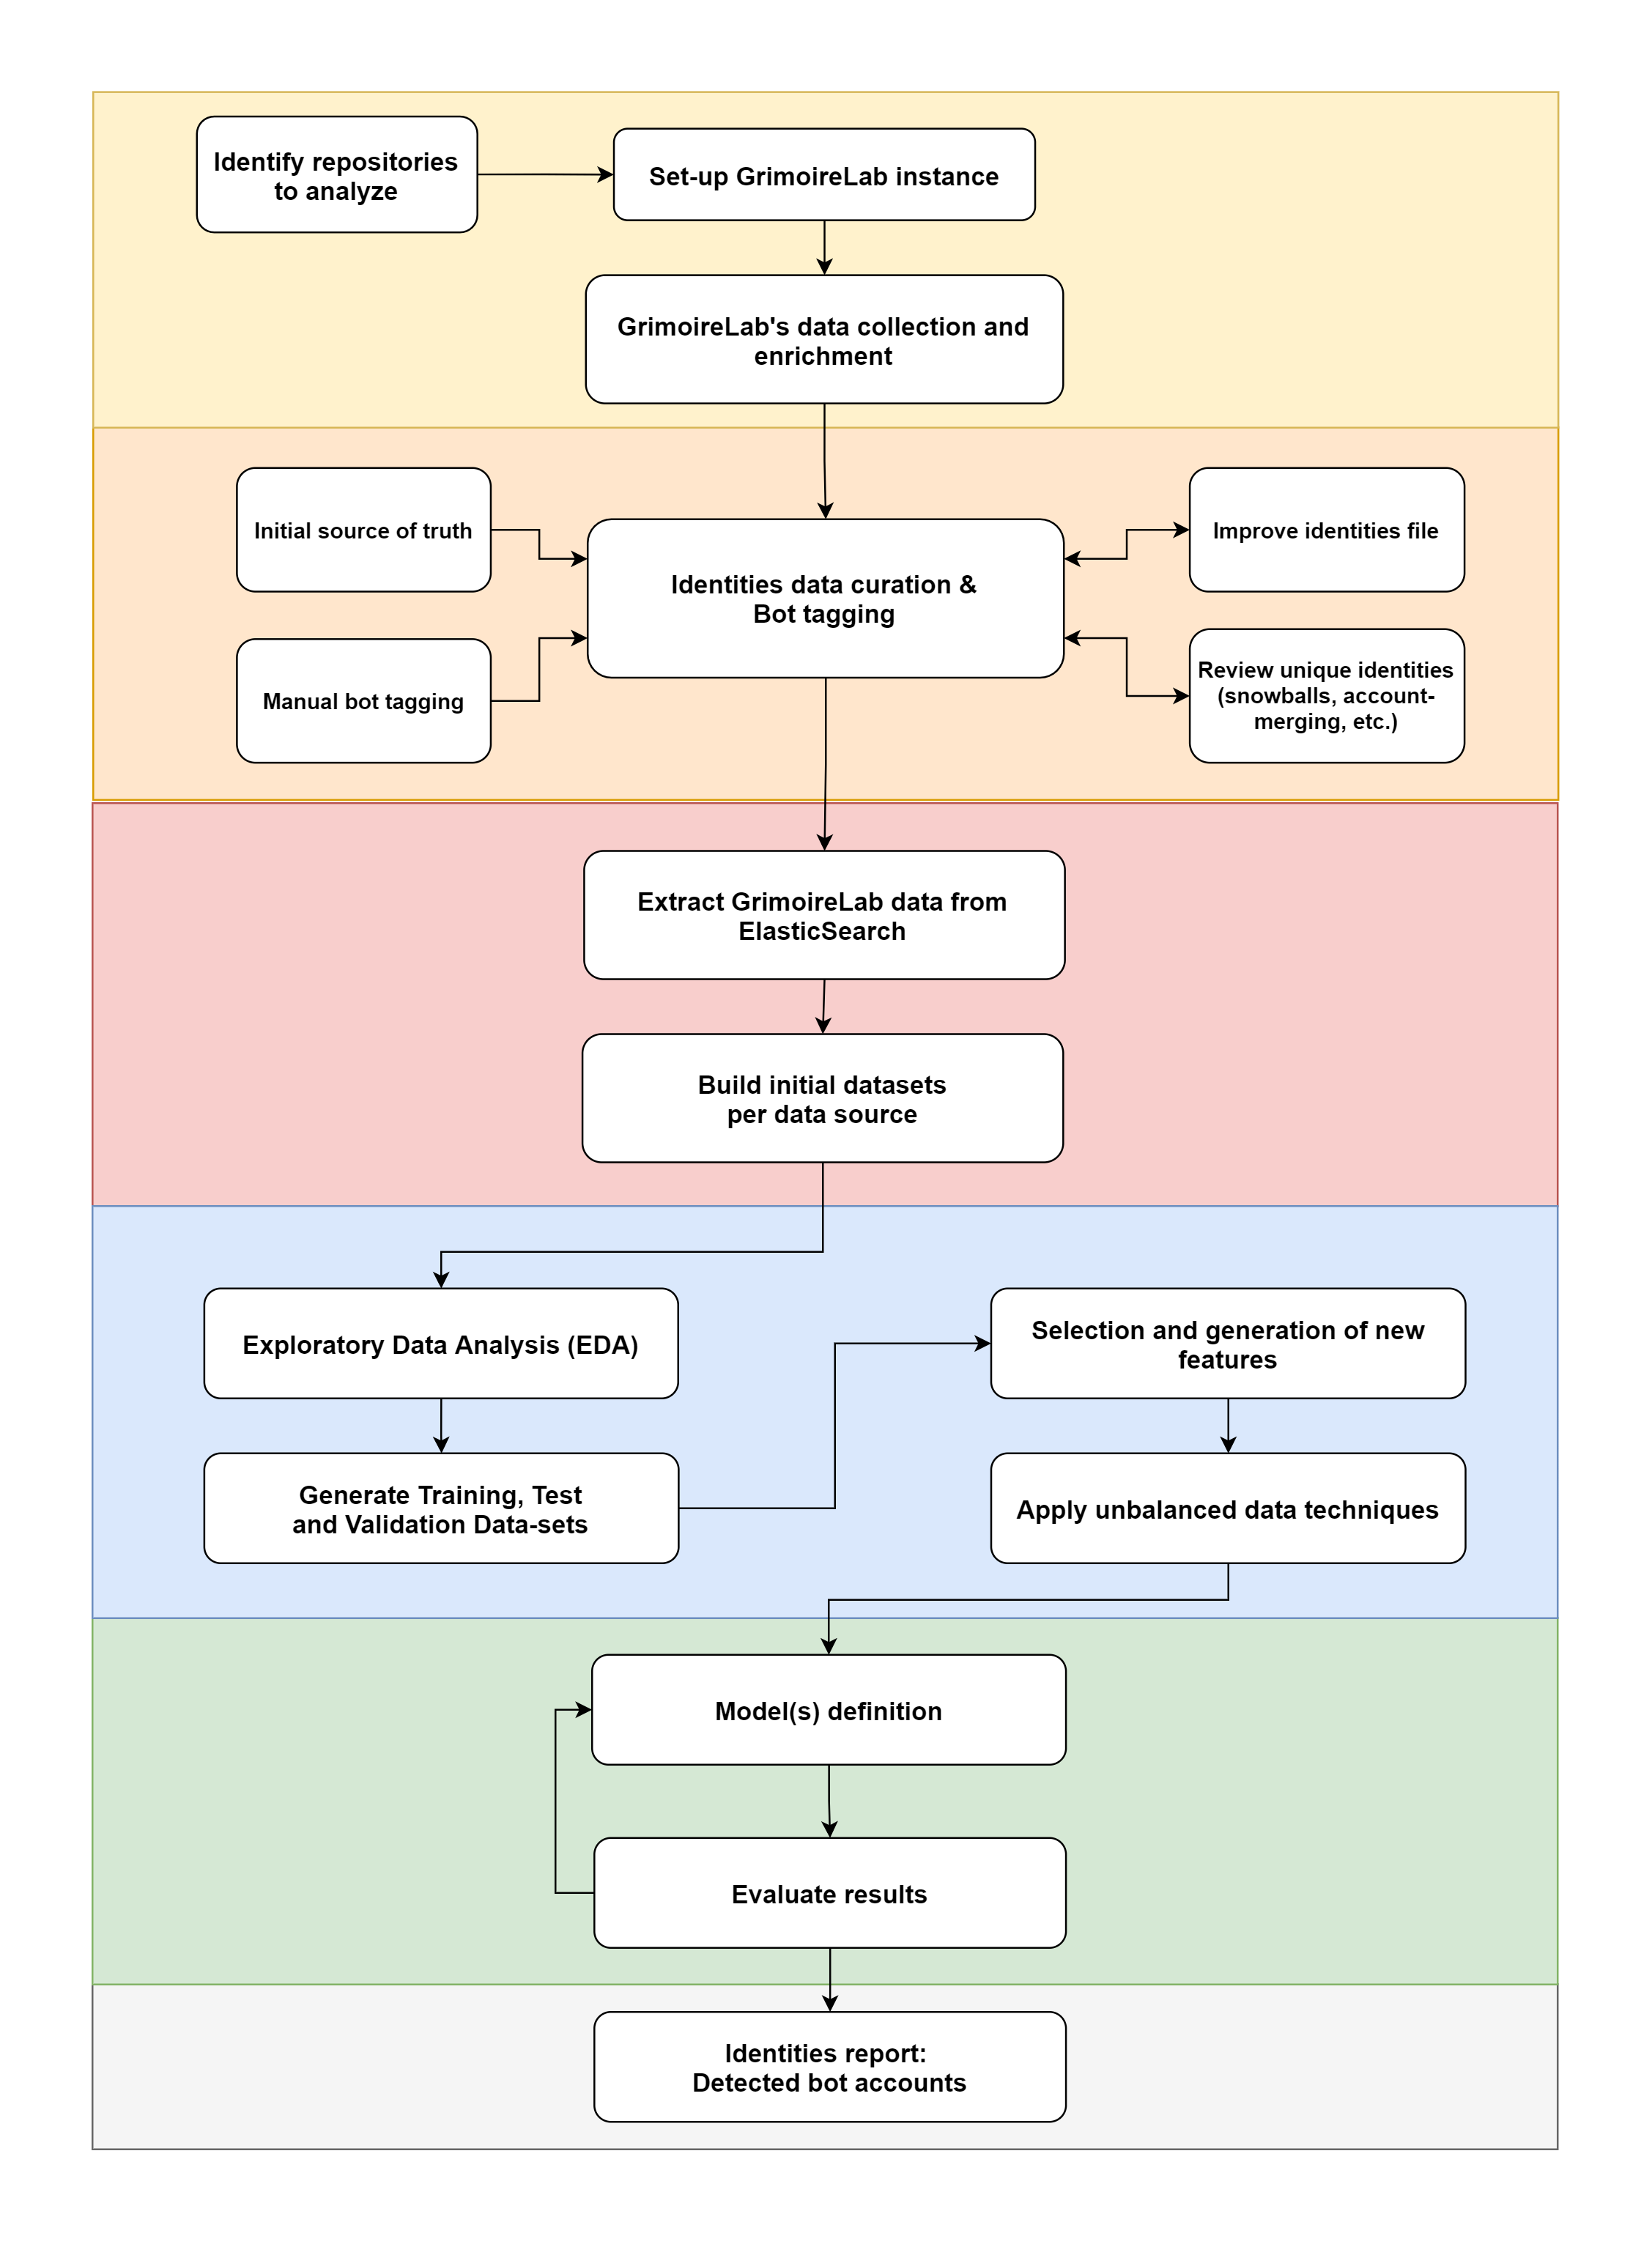
\includegraphics[width=16.5cm, keepaspectratio]{img/sections-architechture-revelio.png}
  \caption{Process architecture.}
  \label{fig:process-arch}
\end{figure}

\section{Creating the initial dataset in GrimoireLab} 
\label{sec:creating-dataset}

\subsection{Selecting the community to analyse}
\label{ssec:selecting-community}
In order to create and test the classification models for this project, an initial dataset was needed. After some research, I chose the Wikimedia Foundation community as the target to analyse, as it is a well-known community with a lot of active projects; many of them using automation tools.

Wikimedia Foundation has the ``Wikimedia Tech community metrics dashboard''\footnote{\url{https://wikimedia.biterg.io/}}, which is a running GrimoireLab instance dedicated to get activity metrics from the Wikimedia Tech community. In their public documentation\footnote{\url{https://www.mediawiki.org/wiki/Community_metrics}} (see Figure~\ref{fig:wikimedia-wiki}) it is linked to the list of repositories they are tracking for their community metrics dashboard.

Looking closer at the type of projects that were tracked, many research projects were observed. Then, I decided to set up a local GrimoireLab instance with a subset of the projects. As the main goal of this project is to detect automated accounts out of human accounts, I decided to apply a first filter to exclude most of Wikimedia's research projects. Research projects usually don't have the desired scale nor the level of activity required for the classification stage. Also, the results could not be as much generalised to other projects and communities.

As for the selected data sources to analyse, this project is focused on the data obtained from Git. Some of the selected repositories were stored on GitHub, others were stored in a Wikimedia-managed Gerrit instance.

\begin{figure}
 \centering
  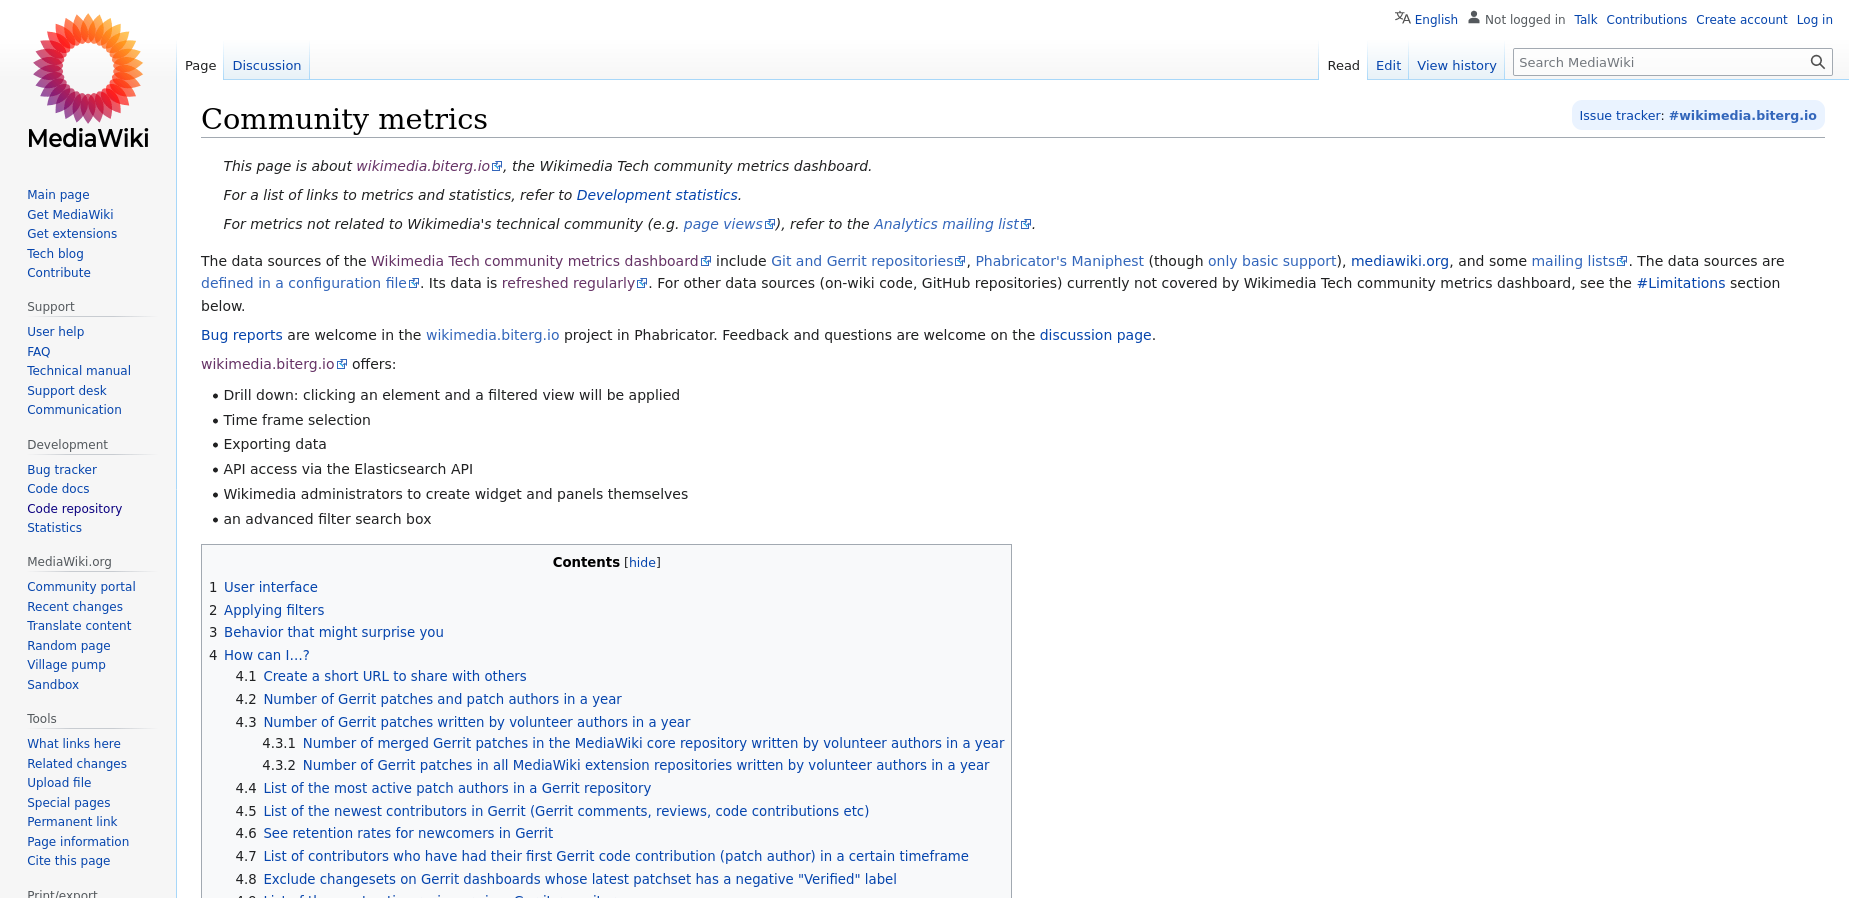
\includegraphics[width=15cm, keepaspectratio]{img/community-metrics-wiki.png}
  \caption{Community Metrics wiki page from Wikimedia Foundation.}
  \label{fig:wikimedia-wiki}
\end{figure}

\subsection{Setting-up the GrimoireLab instance}
\label{ssec:setting-grimoirelab}

With this information, I deployed a local instance of GrimoireLab (Figure~\ref{fig:local-grimoirelab-git}) by using a Docker-compose file available on GrimoireLab repository, configuring the sources file, with the selected subset of repositories to analyse; and the setup configuration file, including:
\begin{itemize}
    \item The name of the instance.
    \item The set-up parameters for the identities' management tool, \emph{SortingHat}.
    \item The name of the ElasticSearch indexes and additional pre-computed studies over the data provided by GrimoireLab.
\end{itemize}

Once the platform is running, GrimoireLab instance performs many operations:
\begin{enumerate}
    \item First, it downloads the raw data from the selected data sources. For this case, to get the data from Git, the repositories from the sources file are downloaded and the Git log file is parsed. This information is stored in JSON documents, one document per ``Commit''.
    \item Then, these documents are processed by another tool that adds additional information such as the number of files modified or the number of total lines added and removed on each commit, or pre-computed fields like time differences. This process is called \textit{data enrichment.}
    \item Besides, identities-related information is aggregated to this extended set of the data (enriched data). That is, each commit is authored by an individual, represented in the identities' database by a unique identifier, an associated profile, and a list of identities belonging to this individual (different email addresses, different GitHub accounts, etc.).
\end{enumerate}

\begin{figure}
 \centering
  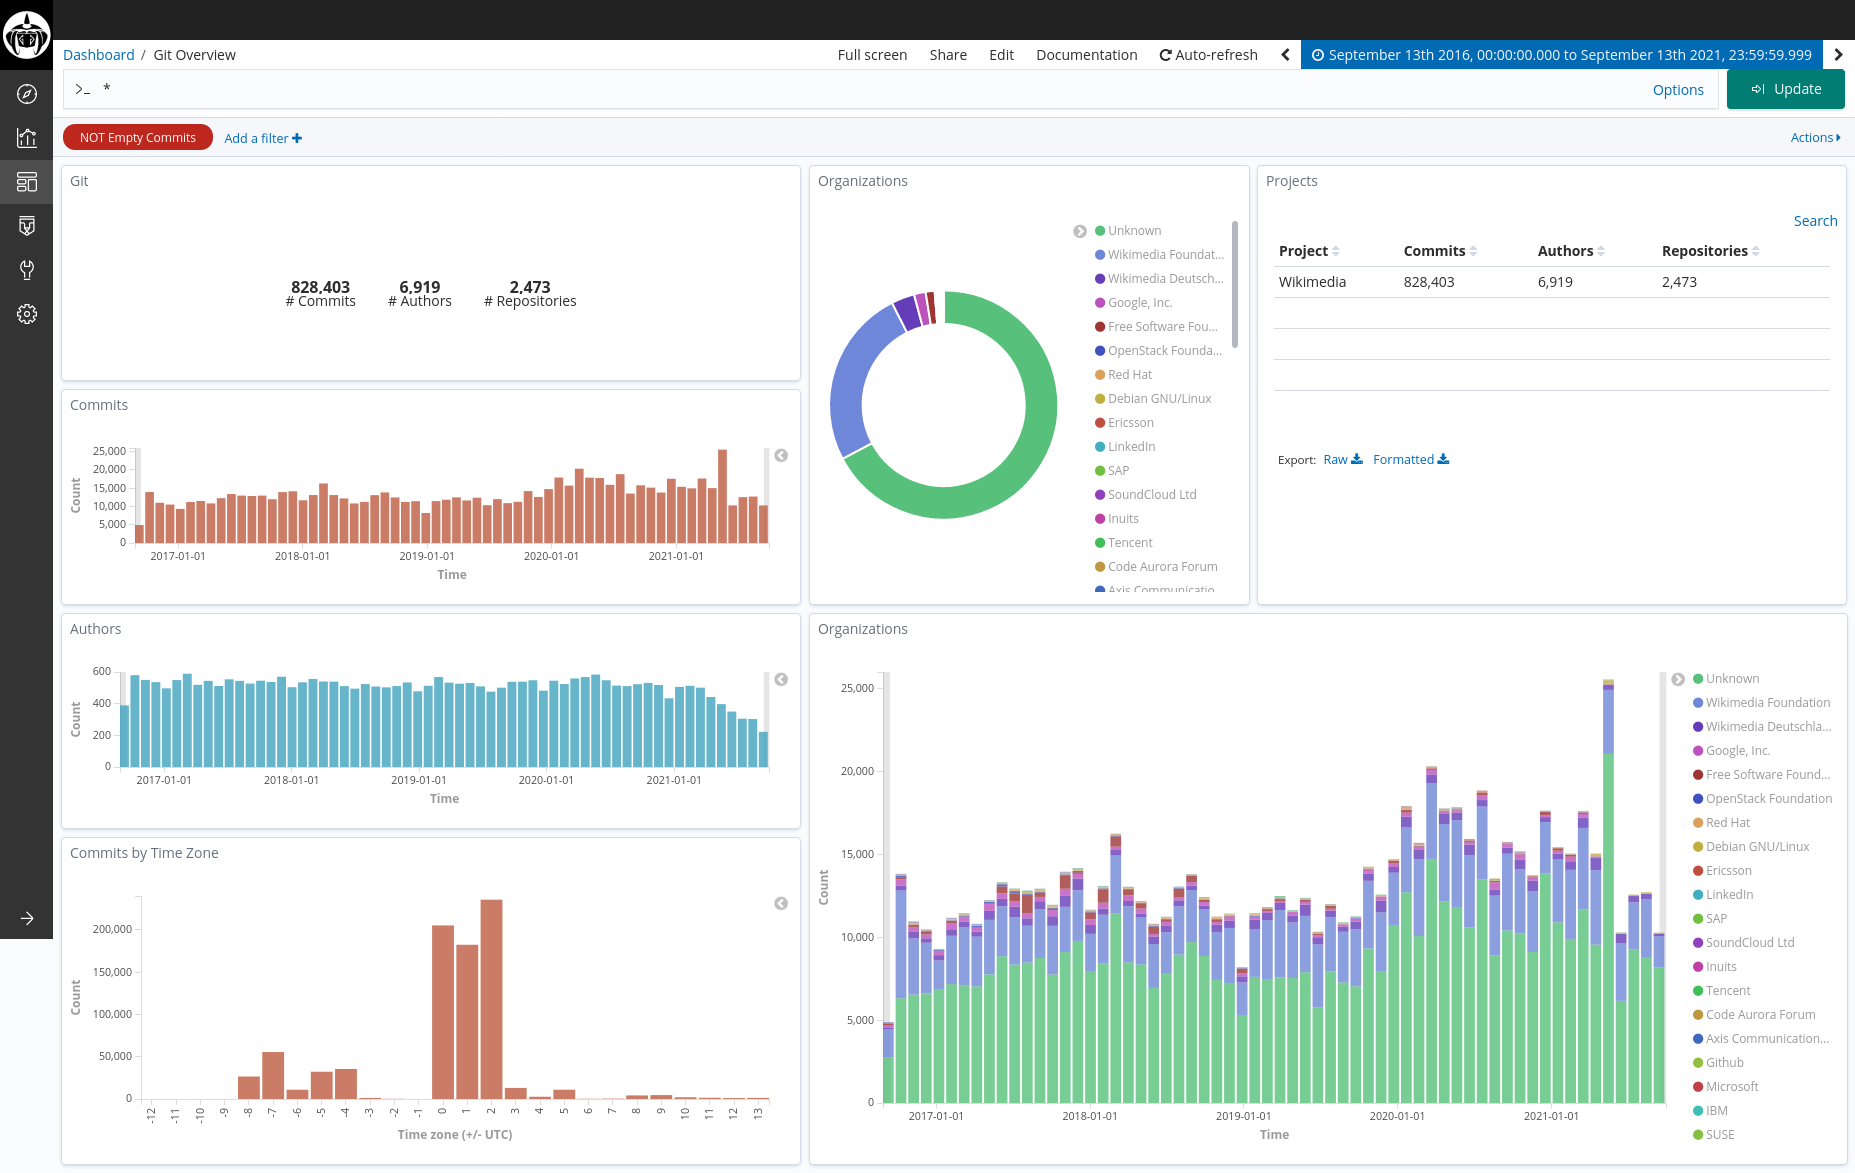
\includegraphics[width=15cm, keepaspectratio]{img/local-instance-grimoirelab-1.png}
  \caption{Dashboard showing the Git data obtained with GrimoireLab locally, after curating identities information.}
  \label{fig:local-grimoirelab-git}
\end{figure}

\subsection{Curating identities information}
\label{ssec:curate-identities}

The next step is to curate the identities' information. The GrimoireLab tool managing this process, SortingHat, offers mechanisms to automatically improve some key data.

Regarding account-merging, SortingHat provides many possibilities to merge profiles based on different fields from individuals (email, name and username) both individually or jointly. As we are not assuming any information, the safest approach was to merge profiles by their email. That is, if there are two or more individuals using the same email account, they are merged into the same profile.

Then, it comes the affiliation information. SortingHat features a way to automatically enrol individuals in an organisation based on the email domain from the profile. This is done by using an organisation-domain map (e.g.: Domain \texttt{wikimedia.org} is linked to the organisation ``\texttt{Wikimedia Foundation}'').

Having said this, SortingHat does not have any automated way to detect which individuals are automatics accounts (\emph{bots}), and this is where \emph{Revelio} tool comes to play.

Two approaches are followed to identify which individuals were bots. The first step consisted of taking all the accounts which were already identified as ``bots'' by the Wikimedia tech community itself in a dedicated Affiliations dashboard\footnote{\url{https://wikimedia.biterg.io/app/kibana\#/dashboard/Affiliations}}, filtering in bot individuals (\texttt{author\_bot:true}) from the \texttt{git} index.

Second, the rest of the individuals are manually reviewed to identify potential bots and then confirm they were looking at their activity. A total of $41$ bot individuals were identified, out of $16,284$. With this information, a SortingHat-supported file is composed with information about each bot individual, for replication purposes.

\section{Data extraction} 
\label{sec:data-extraction}

Before data are extracted from ElasticSearch, it is important to understand how GrimoireLab platform is modelling such data. In this case, we are focusing on Git data.

GrimoireLab downloads each Git repository and parses the Git log (see Figure~\ref{fig:example-commit-github}), storing the entire commits history. From this record per repository, GrimoireLab composes a JSON document per commit, with a set of fields reflecting the information associated with it, such as the unique identifier (\textit{hash}), the number of modified lines, the number of modified files, the commit message, and more (see Listing~\ref{lst:git-elasticsearch}). Later, there is another internal process where these data are augmented with extra fields, such as the identity information matched with data from the identity management system, together with some pre-processed fields that allow aggregating them in a simpler way in Kibana, the visualisation layer from the Elastic stack.

In summary, the \texttt{git} index stores one document per commit, with a set of fields whose meaning is described in the corresponding data schema\footnote{\url{https://github.com/chaoss/grimoirelab-elk/blob/master/schema/git.csv}}.

\begin{figure}
  \centering
  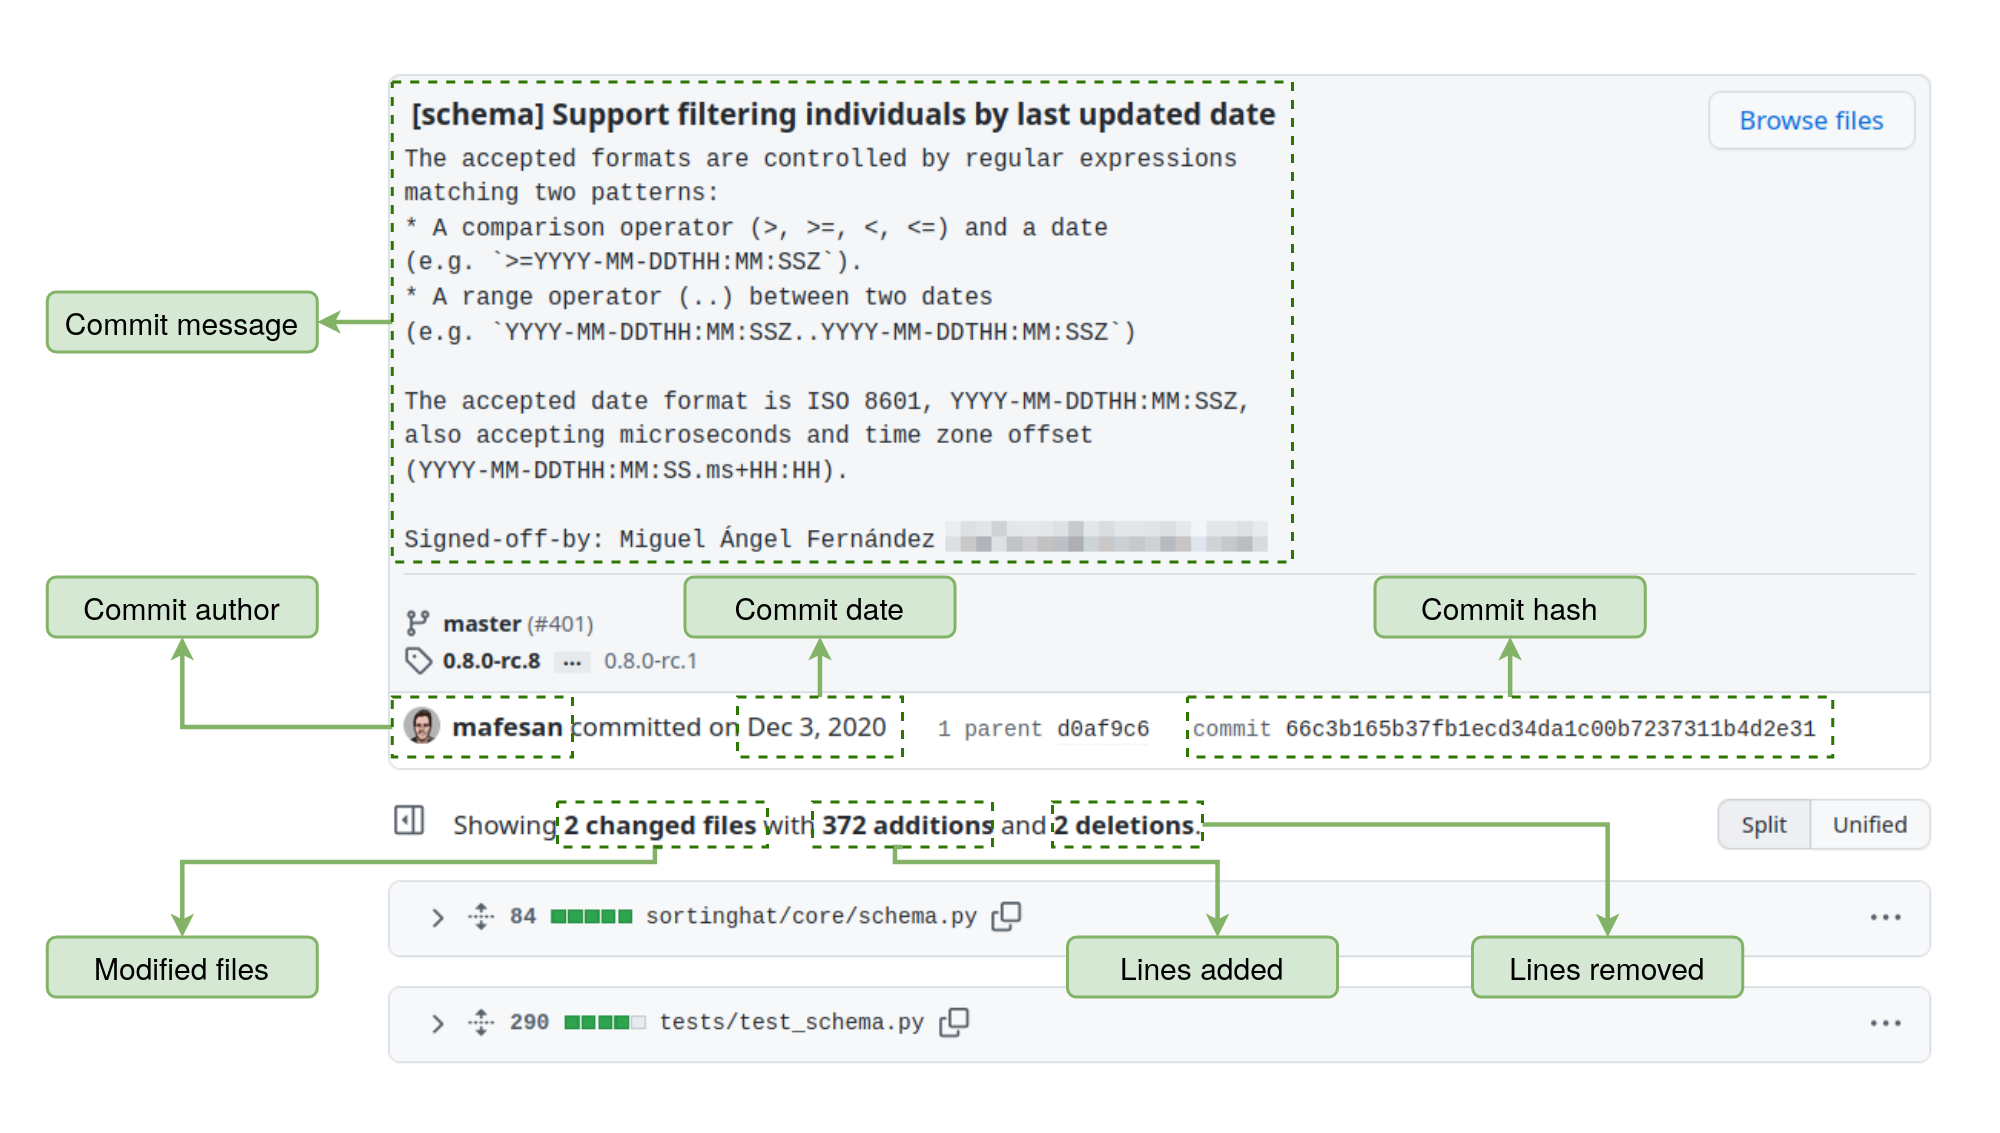
\includegraphics[width=16cm, keepaspectratio]{img/example-commit-mafesan.drawio.png}
  \caption{Graphic example of a Git log entry and some of the information we can extract from it.}
  \label{fig:example-commit-github}
\end{figure}

\begin{listing}[h!]
    \caption{Example of the JSON file per commit produced by GrimoireLab (only the main fields are included).}{}
    \label{lst:git-elasticsearch}
    \begin{minted}[breaklines, fontsize=\footnotesize, baselinestretch=1]{json}
{
    "author_bot": false,
    "author_date": "2020-12-02T13:16:53",
    "author_date_hour": 13,
    "author_date_weekday": 3,
    "author_name": "Miguel Ángel Fernández",
    "author_org_name": "Bitergia",
    "author_user_name": "mafesan",
    "author_uuid": "226b402c4ab1a8a114ff9bd804f4e250c0aa05db",
    "commit_date": "2020-12-03T11:38:49",
    "commit_date_hour": 11,
    "commit_date_weekday": 4,
    "files": 2,
    "github_repo": "chaoss/grimoirelab-sortinghat",
    "grimoire_creation_date": "2020-12-02T13:16:53+01:00",
    "hash": "66c3b165b37fb1ecd34da1c00b7237311b4d2e31",
    "hash_short": "66c3b1",
    "lines_added": 372,
    "lines_changed": 374,
    "lines_removed": 2,
    "message": "[schema] Support filtering individuals by last updated date\n\nThe accepted formats are controlled by regular expressions\nmatching two patterns:\n* A comparison operator (>, >=, <, <=) and a date\n(e.g. `>=YYYY-MM-DDTHH:MM:SSZ`).\n* A range operator (..) between two dates\n(e.g. `YYYY-MM-DDTHH:MM:SSZ..YYYY-MM-DDTHH:MM:SSZ`)\n\nThe accepted date format is ISO 8601, YYYY-MM-DDTHH:MM:SSZ,\nalso accepting microseconds and time zone offset\n(YYYY-MM-DDTHH:MM:SS.ms+HH:HH).\n\nSigned-off-by: Miguel Ángel Fernández <*****@*****>",
    "origin": "https://github.com/chaoss/grimoirelab-sortinghat",
    "project": "GrimoireLab",
    "repo_name": "https://github.com/chaoss/grimoirelab-sortinghat",
    "time_to_commit_hours": 1.63,
    "title": "[schema] Support filtering individuals by last updated date",
    "tz": 1,
    "url_id": "chaoss/grimoirelab-sortinghat/commit/66c3b165b37fb1ecd34da1c00b7237311b4d2e31",
    "utc_commit": "2020-12-03T10:38:49",
}
    \end{minted}
\end{listing}

\subsection{Querying the data from ElasticSearch}
\label{ssec:querying-es}

A set of metrics were defined following the GQM approach~\footnote{These metrics can be found as additional content on the website of the project, in the ``Exploratory Data Analysis'' Notebook.}~\cite{Basili94-gqm}. The next step is selecting the proper fields from the ElasticSearch index that will allow obtaining such metrics, listed in Table~\ref{table:es-git-selected-fields}.

ElasticSearch is a search engine that behaves similarly to a NoSQL database. As the stored entities are single documents, the data need to be aggregated in some way. ElasticSearch has two basic types of aggregations: \textbf{metrics} and \textbf{buckets}. As their documentation explains:
\begin{itemize}
\item The \textbf{metrics} aggregation\footnote{\url{https://www.elastic.co/guide/en/elasticsearch/reference/6.8/search-aggregations-metrics.html}} computes metrics (such as the average, median, unique counts, etc.) based on values extracted in one way or another from aggregated documents. These values are typically extracted from documents fields.
\item The \textbf{buckets} aggregation\footnote{\url{https://www.elastic.co/guide/en/elasticsearch/reference/6.8/search-aggregations-bucket.html}} consists on creating sets of documents (called buckets) taking a given criterion (depending on the aggregation type) which determines whether a document in the current context ``falls'' into it.
\end{itemize} 

The piece of code in charge of retrieving these data is the script \texttt{ES-extract-datasets.py}.

A first process executes a \textit{bucket} aggregation using the unique identifier for the contributor identities, \texttt{author\_uuid}. This first query produces a list of contributors sending commits during a given period of time. Then, a second process executes a query for each author to retrieve the history of commits, asking for the fields that were defined in Table~\ref{table:es-git-selected-fields}. Although results are paginated, this process is split by monthly date ranges from the main time period considered for the study, in this case from January 1st, 2008 to September 15th, 2021.

The output is a set of JSON files, one for each unique contributor, containing the targeted variables for all commits~\ref{fig:example-users-commits-dataset}.

\begin{figure}
  \centering
  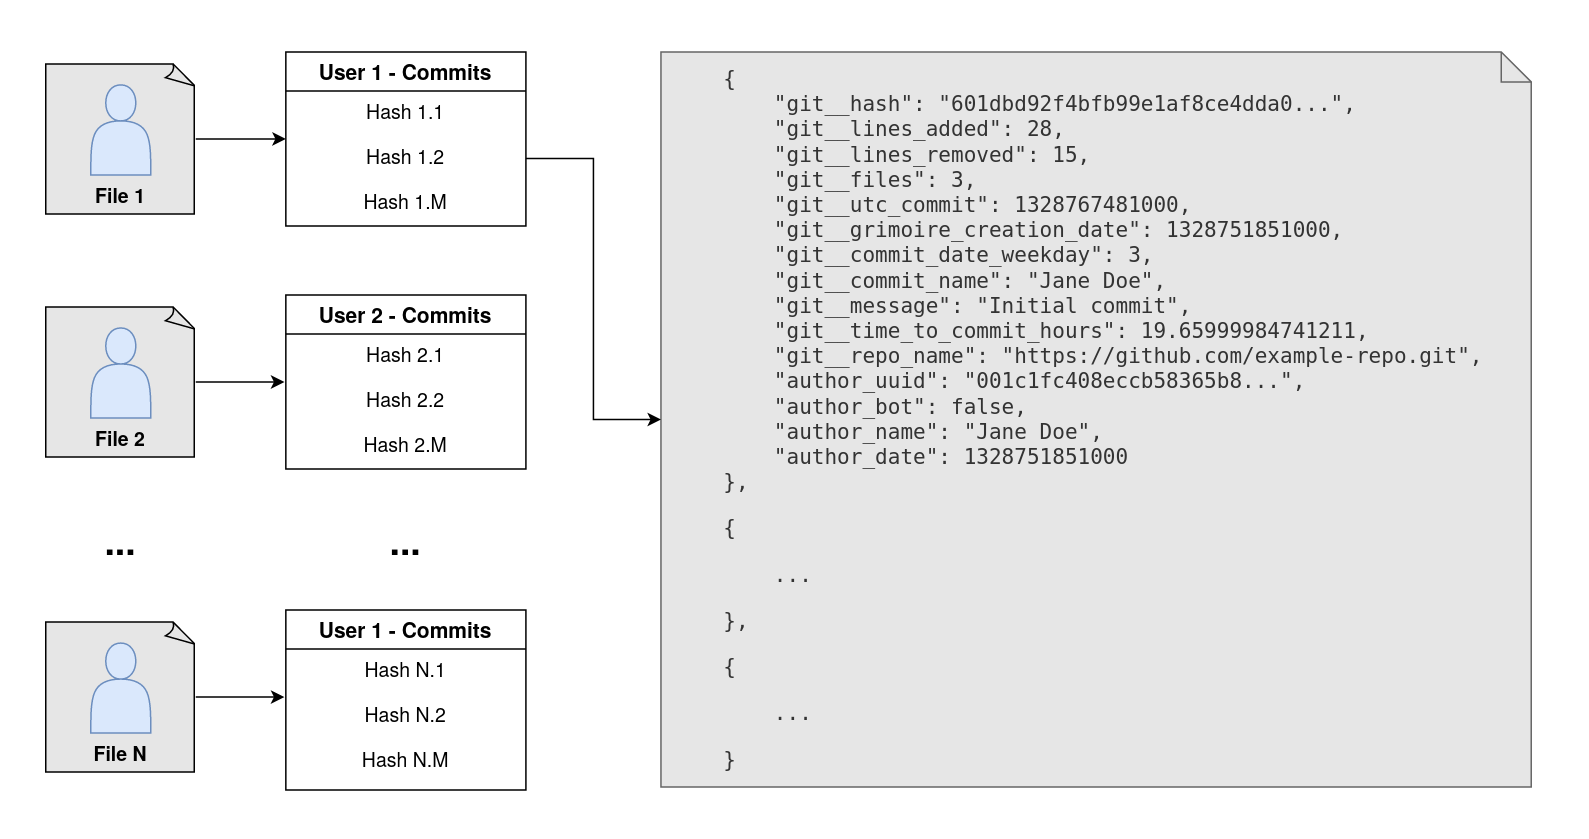
\includegraphics[width=16cm, keepaspectratio]{img/data-files-revelio-users-commits.drawio.png}
  \caption{Graphic example of how data extracted from ElasticSearch look like: one file per author is produced, which contains a set of fields for all of its commits submitted within the time period for the analysis.}
  \label{fig:example-users-commits-dataset}
\end{figure}

\begin{table}[b]  % [htb] suggests table position in page
                    % h: here; t: top; b: bottom
                    % remove any id to restrict options
 \renewcommand{\arraystretch}{1.2}  % Increase space between rows
 \begin{center}
  \begin{tabular}{ l  r }
  % \begin{tabular} { | l | c | r |} % tenemos tres colummnas, la primera alineada a la izquierda (l), la segunda al centro (c) y la tercera a la derecha (r). Se elimina el símbolo |, que indica que entre las columnas habría una línea separadora.
    \toprule    % Top table rule (horizontal) line
      \textbf{Field name} & \textbf{Field description} \\ 
      \midrule % Replace \hline for horizontal rule after table header 
      \texttt{author\_bot} & True if the given author is identified as a bot in SortingHat. \\
      \texttt{author\_date} & Author date (when the original author made the commit). \\
      \texttt{author\_name} & Author name from SortingHat. \\
      \texttt{author\_uuid} & Author UUID from SortingHat. \\
      \texttt{commit\_date\_weekday} & Day of the week when the committer made the commit. \\
      \texttt{commit\_name} & Committer name. \\
      \texttt{files} & Number of files touched by this commit. \\
      \texttt{grimoire\_creation\_date} & Commit date (when the original author made the commit). \\
      \texttt{hash} & Commit hash. \\
      \texttt{lines\_added} & Number of lines added by this commit. \\
      \texttt{lines\_removed} & Number of lines removed by this commit. \\
      \texttt{message} & Commit message as a single String. \\
      \texttt{time\_to\_commit\_hours} & Time in hours from author date to commit date. \\
      \texttt{repo\_name} & Repository the commit was submitted to. \\
      \texttt{utc\_commit} & Commit date in UTC. \\
    \bottomrule     % Bottom table rule (horizontal) line
  \end{tabular}
  \caption{Selected fields from the git index produced by GrimoireLab.}
  \label{table:es-git-selected-fields}
 \end{center}
\end{table}

\subsection{Building the Contributors dataset}
\label{ssec:build-contributors-dataset}

Once having the commit data for all the contributors, the next step is building the main dataset for this project. As the \emph{Revelio} tool is meant to be integrated with SortingHat, the decision was to use the unique individuals as entry values for the classification model, which will predict whether a given contributor is a bot or not.

Our Users-Commits dataset, extracted from GrimoireLab data stored in ElasticSearch, is composed by single commits per author, and our new dataset needs to have one entry per contributor. Thus, we need to represent the information from the history of commits for each author in some way.

Following the metrics defined using the GQM approach, data are processed with a list of variables per contributor, as follows:

\begin{itemize}
\item The unique identifier of the author from SortingHat, used as the index field.
\item The name of the author from SortingHat.
\item The classification of the author as a bot or not, from SortingHat.
\item The number of unique commits.
\item The number of merge commits, which are the ones modifying no files.
\item The number of commits submitted during weekends (either on Saturday or Sunday).
\item The number of commits that have been signed off.
\item The unique number of repositories an author contributed to.
\end{itemize}

Apart from these variables, another set is defined from statistical calculations:
\begin{itemize}
\item The ratio of merge commits, over the total number of commits.
\item The ratio of commits submitted during weekends, over the total number of commits.
\item The ratio of merge commits over the total number of commits.
\item The ratio of signed commits over the total number of commits.
\item The median and the interquartile range for:
    \begin{itemize}
    \item the number of modified files per commit.
    \item the number of added lines per commit.
    \item the number of removed lines per commit.
    \item the length of the commit message.
    \item the number of words (including stop-words)\footnote{Words are counted as groups of characters split by white-space characters within a commit message. Stop-words are preserved, as they could be relevant when analysing patterns.} of the commit messages.
    \end{itemize}
\end{itemize}

The output is a ``Contributors'' dataset, with one row per contributor, including the summarised information from its contributions in the period of
time of the analysis.

\section{Data processing} 
\label{sec:data-processing}

With the ``Contributors'' dataset composed, the next phase consists of exploring the data exhaustively, so it can be consumed by the different classification models we are testing for our problem.

\subsection{Exploratory Data Analysis}
\label{ssec:eda}

For this last set of statistical calculations, a given amount of commits per author is required. In order to avoid considering data from pet projects and casual users (for example, some contributors only submit a small number of contributions as part of a learning course), an additional criterion is to ignore those authors having less than $10$ commits for the selected time period. 

After applying this first rule, the starting point is a dataset composed of $3,747$ rows, one for each contributor.

Looking at the statistical distribution of the variable we aim to classify, \texttt{author\_bot} in Figure~\ref{fig:eda-contributors-bot-proportion}, it can be concluded that this is a highly unbalanced dataset: from these $3,747$ contributors, only $30$ are marked as bots. This must be taken into account when creating the training, test, and validation datasets, and it also implies additional data processing in order to mitigate the effects of such an imbalance on the different classification models.

\begin{figure}
 \centering
  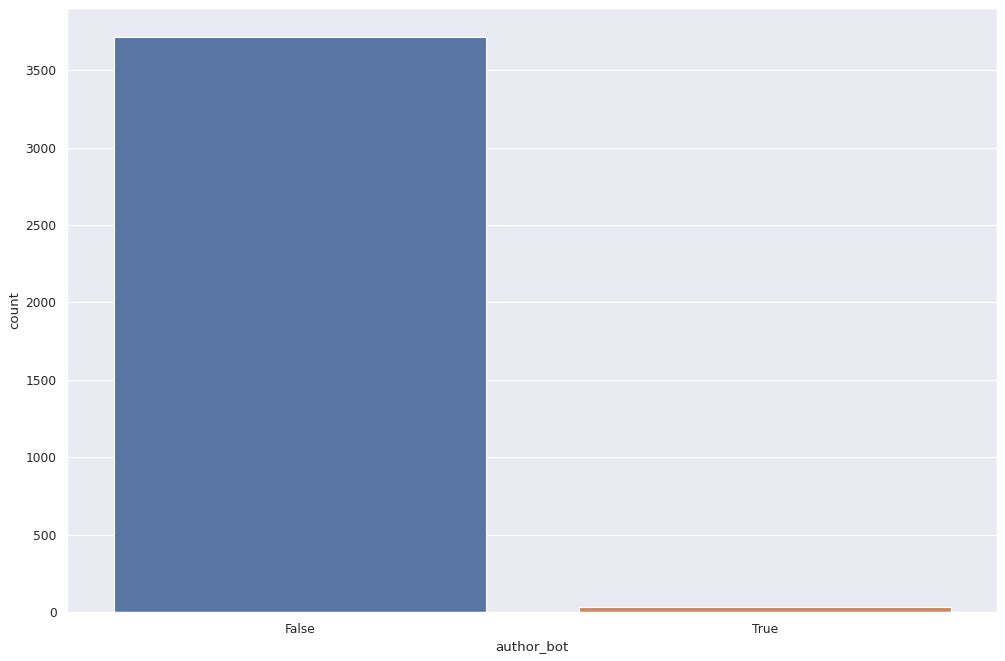
\includegraphics[width=15cm, keepaspectratio]{img/authors_bots_proportion.png}
  \caption{Proportion of contributors marked as a bot (False, on the left; True on the Right).}
  \label{fig:eda-contributors-bot-proportion}
\end{figure}

The remaining variables also have very uneven statistical distributions, except for the generated variables (median and interquartile range) for the length of the commit messages. This situation entails these variables should be transformed in order to approximate their distributions to a normalised version of themselves.

Furthermore, another issue to ponder is how these variables were generated as a summary of the activity of each contributor, which is independent, no relative information from other contributors is used to build them. Nonetheless, some of the numerical variables are not completely independent, as they were created to represent extra layers of information inferred from some of the other values, such as the variables counting the number of commits submitted during weekends, which is a subset of the information provided by the variable counting the total number of commits; or those whose value is a relative value computed as a ratio.

\subsection{Building the training, test, and validation datasets}
\label{ssec:build-training-datasets}

The main dataset needs to be split into subsets for the classification stage: one for training ($60\%$ of the samples), one for testing ($25\%$ of the samples), and another one for validation ($15\%$ of the samples), as it is represented in Figure~\ref{fig:dataset-percentages}. 

These subsets need to be statistically similar, so the sample needs to be stratified in order to keep the human/bot proportion. The method \texttt{train\_test\_split} from Scikit-Learn's \texttt{model\_selection} module was used to obtain these subsets, by using the option \texttt{stratify}.

\begin{figure}
 \centering
  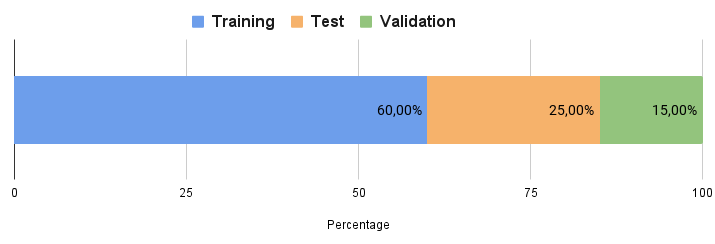
\includegraphics[width=16cm, keepaspectratio]{img/dataset-percentages.png}
  \caption{How the initial dataset was split (stratified) into Training, Test, and Validation sets, showing the percentage each of them represents out of the whole set.}
  \label{fig:dataset-percentages}
\end{figure}

\subsection{Generation and selection of features}
\label{ssec:selection-features}

In this subsection, it is explained how the variables from the Users-Commits dataset have been transformed and selected for serving as the input for the classification models.

\subsubsection{Detection and processing of missing data}
\label{sssec:missing-data}
The data are provided by the GrimoireLab tool set, and the dataset is a collection of information from Git commits. The fields and the information per commit are expected to be standard. 

As we are building in a later step a custom dataset summarising information per author, we are not having missing data except for author-related information, such as the author's name, username, or email (at least one of these three variables has to have a non-empty value).

\subsubsection{Transformation of quantitative variables}
\label{sssec:transformation-quantitative}

The main variables from the dataset are generated in subsection~\ref{ssec:build-contributors-dataset}, and most of them are quantitative variables, as they are representing a summary of the information obtained from the set of commits submitted by each unique author.

The first examination during the Exploratory Data Analysis phase (\ref{ssec:eda}) shows that most of these quantitative variables have remarkably
uneven statistical distributions. There are huge differences in the ranges of values, and also these values are widespread. Under this situation, the
approximation to take was to apply mathematical functions helping to scale these values. Although several transformations were tested, most of the 
variables have been transformed using a customised logarithmic function (see Section~\ref{sec:form-one-plus-log10}) or the squared root function.
The Table~\ref{table:transformation-quantitative} summarises how the variables were transformed. 

\begin{table}[htb]  % [htb] suggests table position in page
                    % h: here; t: top; b: bottom
                    % remove any id to restrict options
 \renewcommand{\arraystretch}{1.2}  % Increase space between rows
 \begin{center}
  \begin{tabular}{ l l }
  % \begin{tabular} { | l | c | r |} % tenemos tres colummnas, la primera alineada a la izquierda (l), la segunda al centro (c) y la tercera a la derecha (r). Se elimina el símbolo |, que indica que entre las columnas habría una línea separadora.
    \toprule    % Top table rule (horizontal) line
    \textbf{Transformation} & \textbf{Feature}\\
    \midrule
    $Log_{10}(x)$       & \texttt{git\_\_num\_commits} \\
                        & \texttt{git\_\_num\_repos} \\
    \addlinespace
    $\sqrt{x}$          & \texttt{git\_\_ratio\_merge\_commits} \\
                        & \texttt{git\_\_ratio\_weekend\_commits} \\
                        & \texttt{git\_\_ratio\_signed\_commits} \\
    \addlinespace
    $Log_{10}(1 + x)$   & \texttt{git\_\_num\_merge\_commits} \\
                        & \texttt{git\_\_num\_weekend\_commits} \\
                        & \texttt{git\_\_num\_signed\_commits} \\
                        & \texttt{git\_\_median\_files} \\
                        & \texttt{git\_\_iqr\_files} \\
                        & \texttt{git\_\_median\_lines\_added} \\
                        & \texttt{git\_\_iqr\_lines\_added} \\
                        & \texttt{git\_\_median\_lines\_removed} \\
                        & \texttt{git\_\_iqr\_lines\_removed} \\
                        & \texttt{git\_\_median\_len\_commit\_message} \\
                        & \texttt{git\_\_iqr\_len\_commit\_message} \\
                        & \texttt{git\_\_median\_len\_words\_commit\_message} \\
                        & \texttt{git\_\_iqr\_len\_words\_commit\_message} \\
    \bottomrule     % Bottom table rule (horizontal) line
  \end{tabular}
  \caption{Transformation applied to quantitative variables.}
  \label{table:transformation-quantitative}
 \end{center}
\end{table}

\subsubsection{Transformation of qualitative variables}
\label{sssec:transformation-qualitative}

Although most of the variables from this dataset are quantitative, the statistical distribution of some of them points to a need to generate 
qualitative, binary variables which derive from them. Looking at the graphical representations\footnote{These graphs are available in the ``Exploratory Data Analysis'' Notebook, in the project's code repository.}, the referenced variables counting the number of commits under a given condition usually have some bias: observing the statistical distribution, the general rule is finding  a peak at $0$ and then the rest of results are very spread over the histogram. 

Following this reasoning, these variables were transformed into binary variables, with the intention of translating the major difference between these values in a conceptual way: For instance, looking at the number of \textit{merge} commits, instead of counting how many of them there are, it could be enough to know just if a given author submitted merge commits or not.

\begin{table}[htb]  % [htb] suggests table position in page
                    % h: here; t: top; b: bottom
                    % remove any id to restrict options
 \renewcommand{\arraystretch}{1.2}  % Increase space between rows
 \begin{center}
  \begin{tabular}{ c }
  % \begin{tabular} { | l | c | r |} % tenemos tres colummnas, la primera alineada a la izquierda (l), la segunda al centro (c) y la tercera a la derecha (r). Se elimina el símbolo |, que indica que entre las columnas habría una línea separadora.
    \toprule    % Top table rule (horizontal) line
    \textbf{Common terms} \\
    \midrule
    \texttt{auto}, \texttt{bot}, \texttt{build}, \texttt{cd}, \texttt{ci}, \texttt{code}, \texttt{commit}, \texttt{copy},\\
    \texttt{dependency}, \texttt{fix}, \texttt{integration}, \texttt{issue}, \texttt{merge}, \texttt{patrol}, \texttt{pr},\\
    \texttt{pull}, \texttt{release}, \texttt{request}, \texttt{review}, \texttt{sync}, \texttt{template}, \texttt{tool}, and \texttt{travis}. \\
    \bottomrule     % Bottom table rule (horizontal) line
  \end{tabular}
  \caption{Common terms used for the name, email, and/or username of automatic accounts.}
  \label{table:common-bot-terms}
 \end{center}
\end{table}

On the other hand, I composed a list of heuristic terms (see Table~\ref{table:common-bot-terms}) belonging to the application domain, using the terminology of tasks that bots are usually performing during the software development process.  The first approach was to create a set of dummy variables with one column per term, where the value is $1$ (\textbf{True}) when the term from that column is included in the author's name; and $0$ (\textbf{False}) if it is not included. For instance, a user named \texttt{ghmerger} would have a $1$ value in the `merge` and `merger` columns, and a $1$ value in the rest of the columns. 

Nonetheless, this approach was adding too much complexity to the system. After several experiments from Chapter~\ref{chap:experiments}, the decision was to summarise the inclusion of these terms into a ``terms score''. The idea was to classify the heuristic terms in three different levels assigning weights to each of them, according to their relevance in the application domain. Doing so, an author name having one or more terms from the list would have a greater value, also taking into account their relevance by using these levels. Having a score of $0$ means the \texttt{author\_name} field doesn't include any of the relevant terms. The formula to compute this terms score is available at Section~\ref{sec:terms-score-definition}, and the definition of these three levels is available at Table~\ref{table:levels-bot-terms}. 

\begin{table}[htb]  % [htb] suggests table position in page
                    % h: here; t: top; b: bottom
                    % remove any id to restrict options
 \renewcommand{\arraystretch}{1.2}  % Increase space between rows
 \begin{center}
  \begin{tabular}{ l c r }
  % \begin{tabular} { | l | c | r |} % tenemos tres colummnas, la primera alineada a la izquierda (l), la segunda al centro (c) y la tercera a la derecha (r). Se elimina el símbolo |, que indica que entre las columnas habría una línea separadora.
    \toprule    % Top table rule (horizontal) line
    \textbf{Level} & \textbf{Weight} & \textbf{Heuristic terms} \\
    \midrule
    $1$ & $60$ & \texttt{bot}, \texttt{dependency}, \texttt{fix},  \texttt{integration} and \texttt{merge} \\
    \addlinespace
    $2$ & $30$ & \texttt{auto}, \texttt{build}, \texttt{commit}, \texttt{copy}, \texttt{issue}, \texttt{release}, \texttt{request}, \\
     & & \texttt{review}, \texttt{sync}, \texttt{template}, \texttt{tool} and \texttt{travis} \\
    \addlinespace
    $3$ & $10$ & \texttt{cd}, \texttt{ci}, \texttt{code}, \texttt{patrol}, \texttt{pr}, and \texttt{pull} \\
    \bottomrule     % Bottom table rule (horizontal) line
  \end{tabular}
  \caption{Levels of heuristic terms and their assigned weights used for computing a term score.}
  \label{table:levels-bot-terms}
 \end{center}
\end{table}

As a final note, our target variable \texttt{author\_bot} is also a categorical, binary variable, as it is a property given by the GrimoireLab platform (the variable es $1$ when a given author is marked as an automatic account in SortingHat, and $0$ otherwise).

\begin{table}[htb]  % [htb] suggests table position in page
                    % h: here; t: top; b: bottom
                    % remove any id to restrict options
 \renewcommand{\arraystretch}{1.2}  % Increase space between rows
 \begin{center}
  \begin{tabular}{ l l }
  % \begin{tabular} { | l | c | r |} % tenemos tres colummnas, la primera alineada a la izquierda (l), la segunda al centro (c) y la tercera a la derecha (r). Se elimina el símbolo |, que indica que entre las columnas habría una línea separadora.
    \toprule    % Top table rule (horizontal) line
    \textbf{Transformed feature} & \textbf{Meaning} \\
    \midrule
    \texttt{git\_\_has\_merge\_commits}   & $1$ if a given author has submitted at least one\\
                                          & merge commit; $0$ otherwise.\\
    \addlinespace
    \texttt{git\_\_has\_weekend\_commits} & $1$ if a given author has submitted at least one\\                                          & commit during Saturday or Sunday; $0$ otherwise.\\
    \addlinespace
    \texttt{git\_\_has\_signed\_commits}  & $1$ if a given author has submitted at least one\\
                                          & signed commit; $0$ otherwise.\\
    \addlinespace
    \texttt{terms\_score} & Integer value representing a score obtained from the\\
                          & author's name, computed as detailed in Section~\ref{sec:terms-score-definition}.\\
    \bottomrule     % Bottom table rule (horizontal) line
  \end{tabular}
  \caption{Transformation of qualitative variables.}
  \label{table:transformation-qualitative}
 \end{center}
\end{table}


\subsection{Correlation}
\label{ssec:correlation}

To study the correlation between the variables in the dataset, in Figure~\ref{fig:corr-heatmap-before} it is represented a correlation matrix with absolute values, taking into account the dataset with the transformed variables. 

By representing the correlation matrix it was revealed there was a set of variables with high correlation values. The decision was to establish a hard threshold on correlation values greater than $0.75$. In Figure~\ref{fig:corr-heatmap-greater-075}, it is shown the pairs of variables which have correlation values above the threshold. After studying the relevance given the application domain; and also having into account that there were some variables that seemed redundant (the values from both the interquartile range and the median had a high correlation in most cases), the following variables were removed from the transformed dataset: 
\begin{itemize}
\item \texttt{git\_\_sqrt\_ratio\_merge\_commits}
\item \texttt{git\_\_sqrt\_ratio\_weekend\_commits}
\item \texttt{git\_\_sqrt\_ratio\_signed\_commits}
\item \texttt{git\_\_log\_iqr\_lines\_added}
\item \texttt{git\_\_log\_iqr\_lines\_removed}
\item \texttt{git\_\_log\_iqr\_len\_commit\_message}
\item \texttt{git\_\_log\_median\_len\_words\_commit\_message}
\end{itemize}

After these changes, the correlation values from the resulting dataset are detailed in Figure~\ref{fig:corr-heatmap-after}.



\begin{figure}
 \centering
  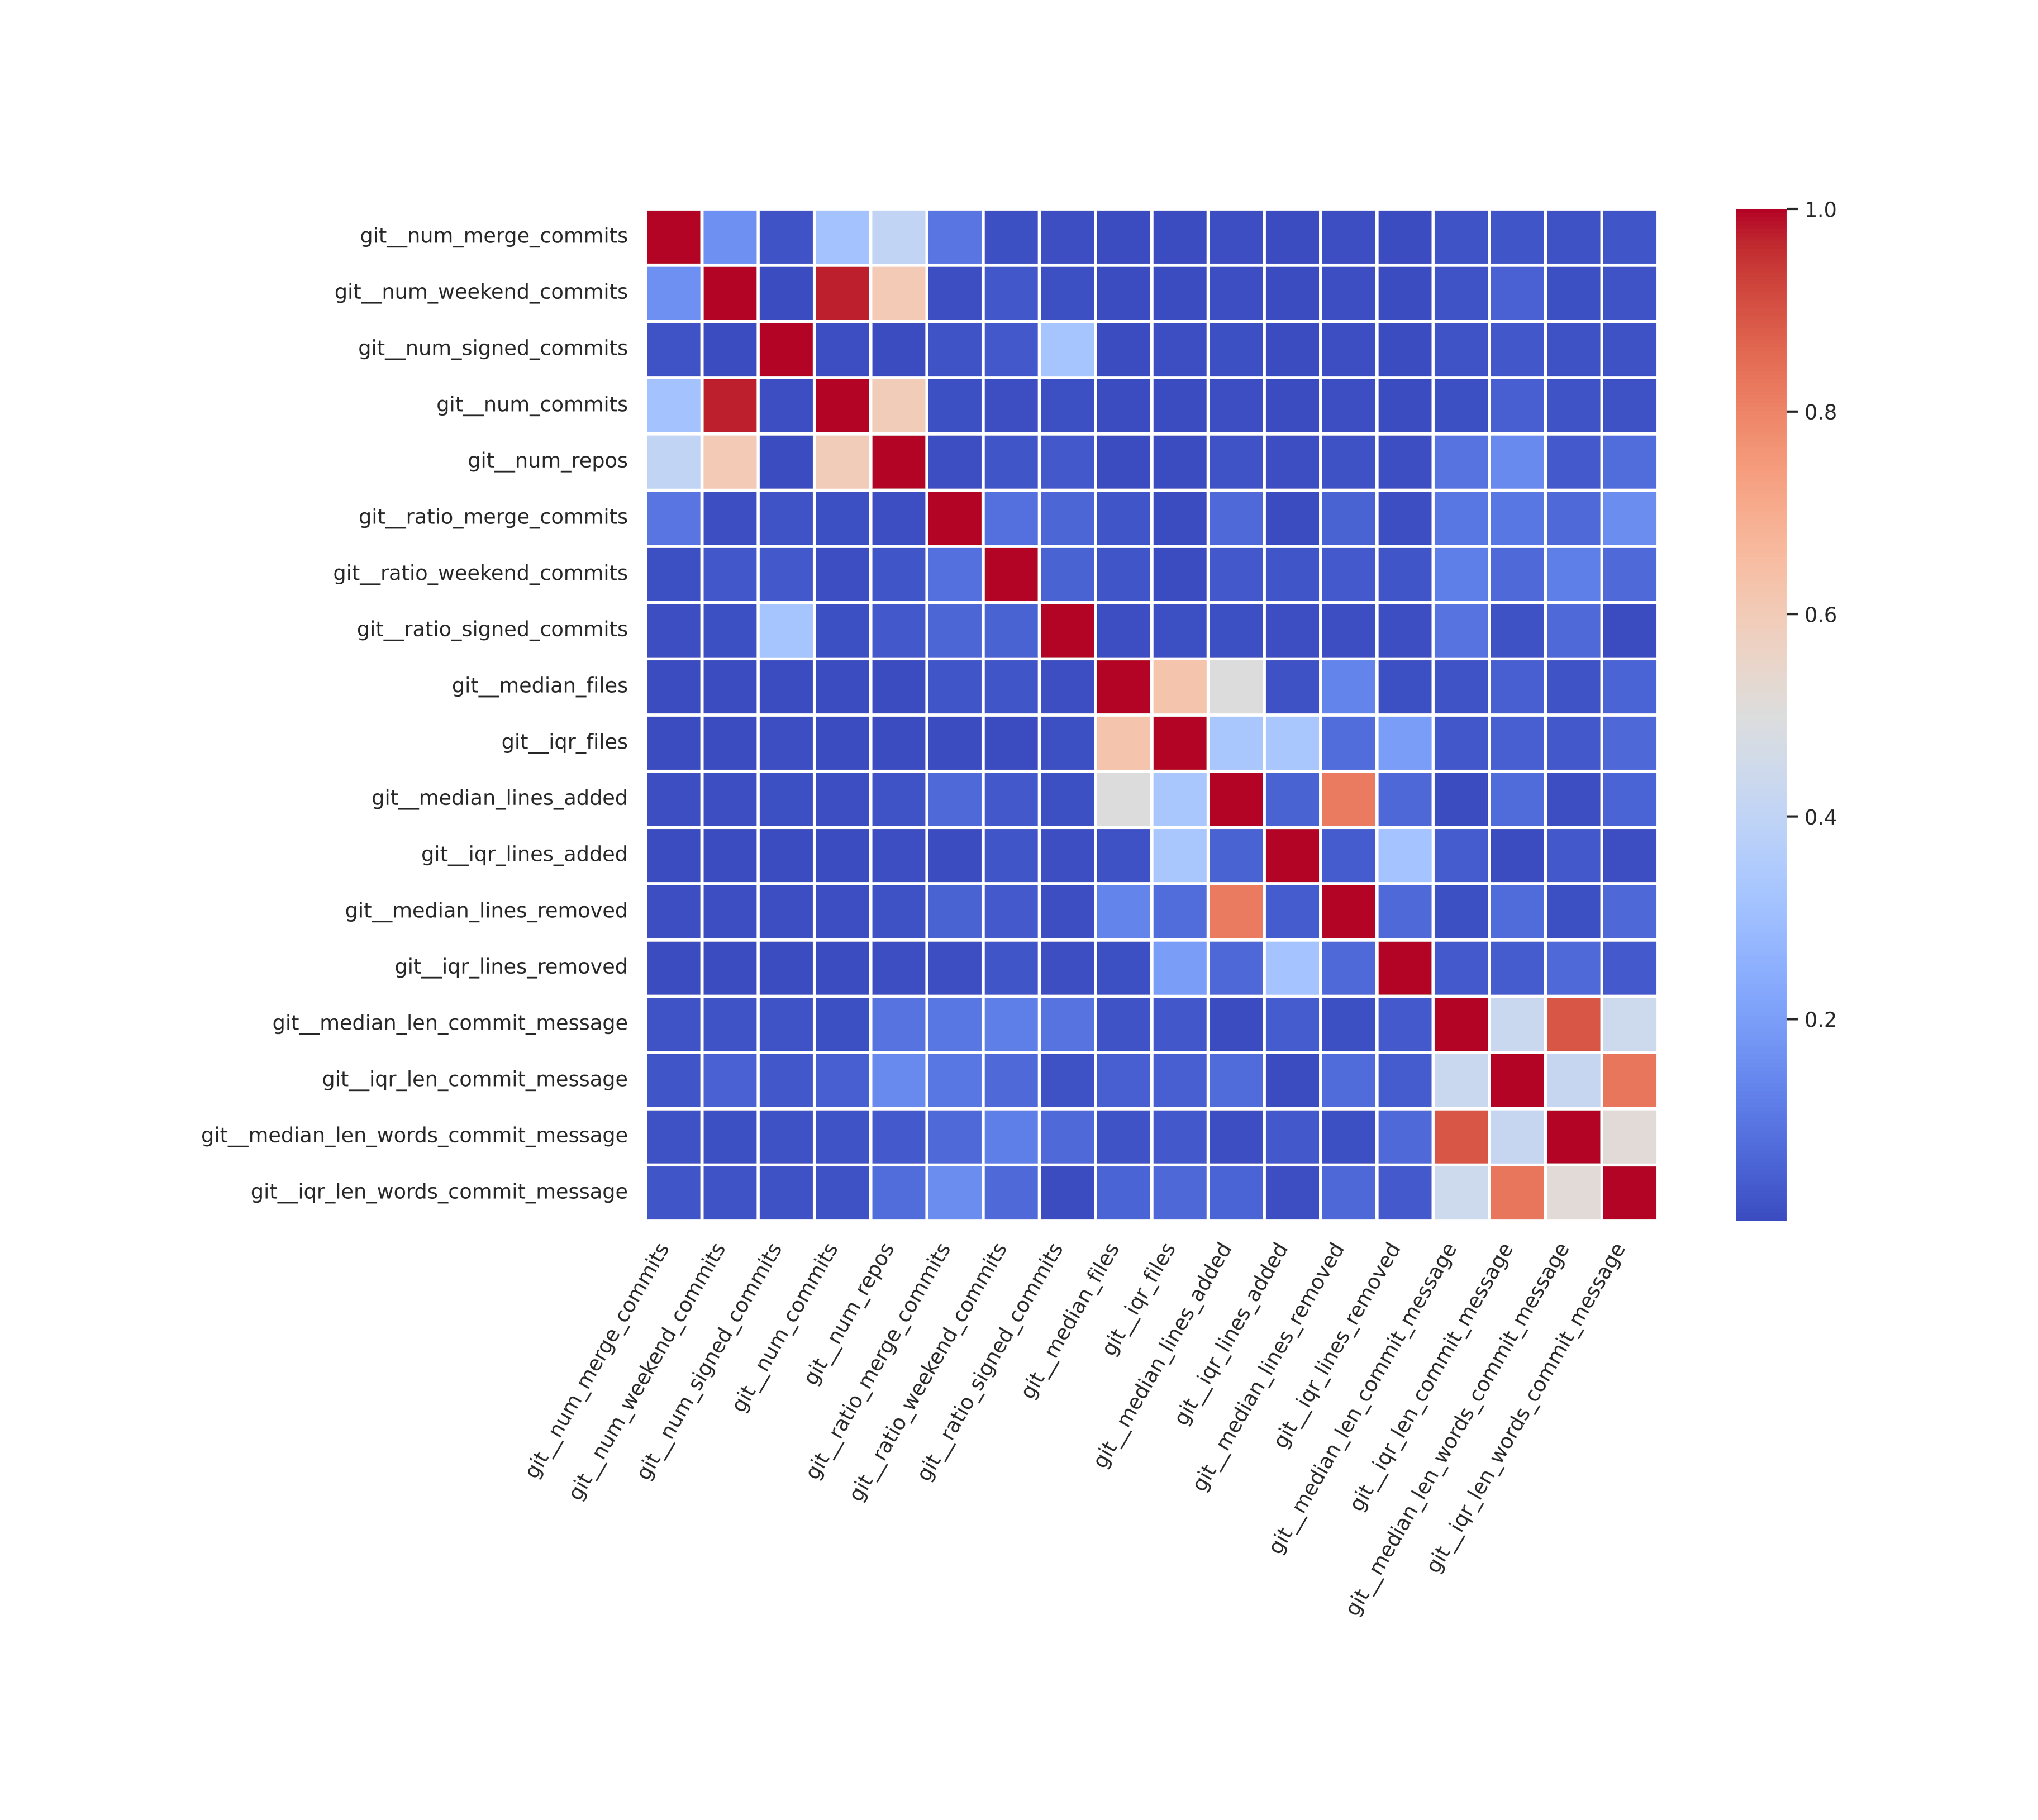
\includegraphics[width=18cm, keepaspectratio]{img/eda_corr_heatmap_before.png}
  \caption{Correlation heat map of the initial variables from the training dataset.}
  \label{fig:corr-heatmap-before}
\end{figure}

\begin{figure}
 \centering
  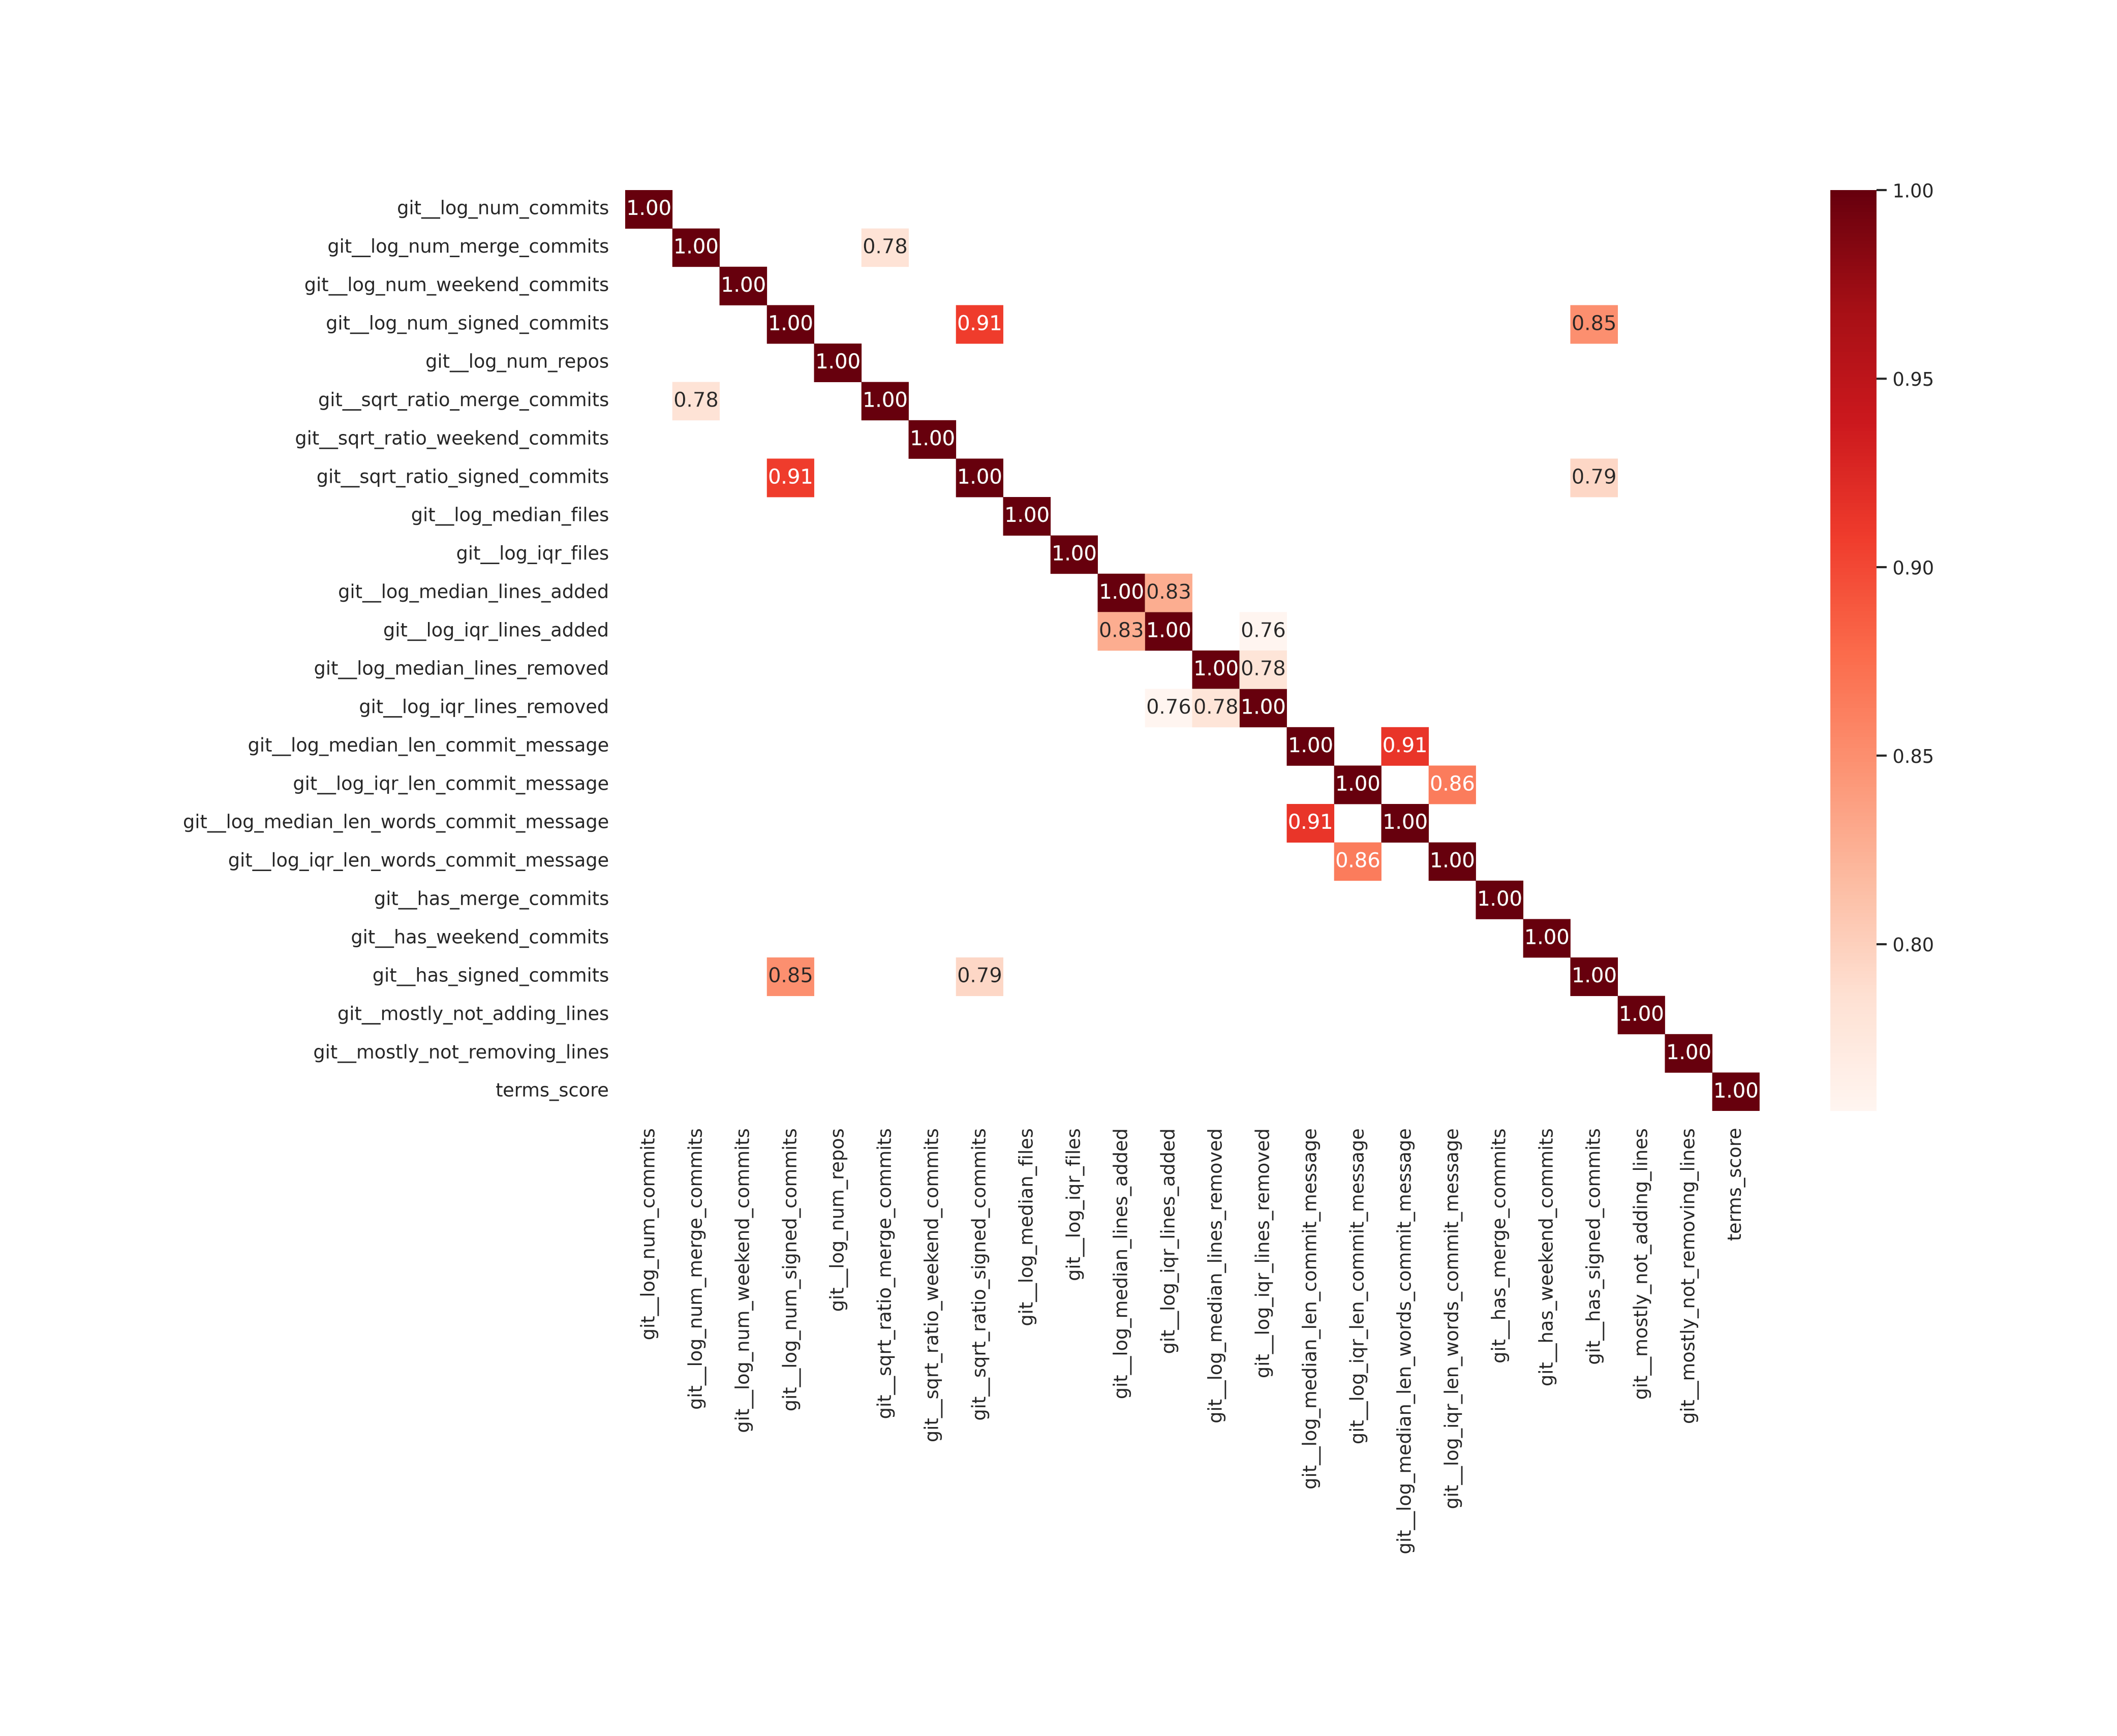
\includegraphics[width=18cm, keepaspectratio]{img/eda_corr_heatmap_more_75.png}
  \caption{Correlation heat map showing the pairs of variables with an absolute correlation greater than $0.75$ .}
  \label{fig:corr-heatmap-greater-075}
\end{figure}


\begin{figure}
 \centering
  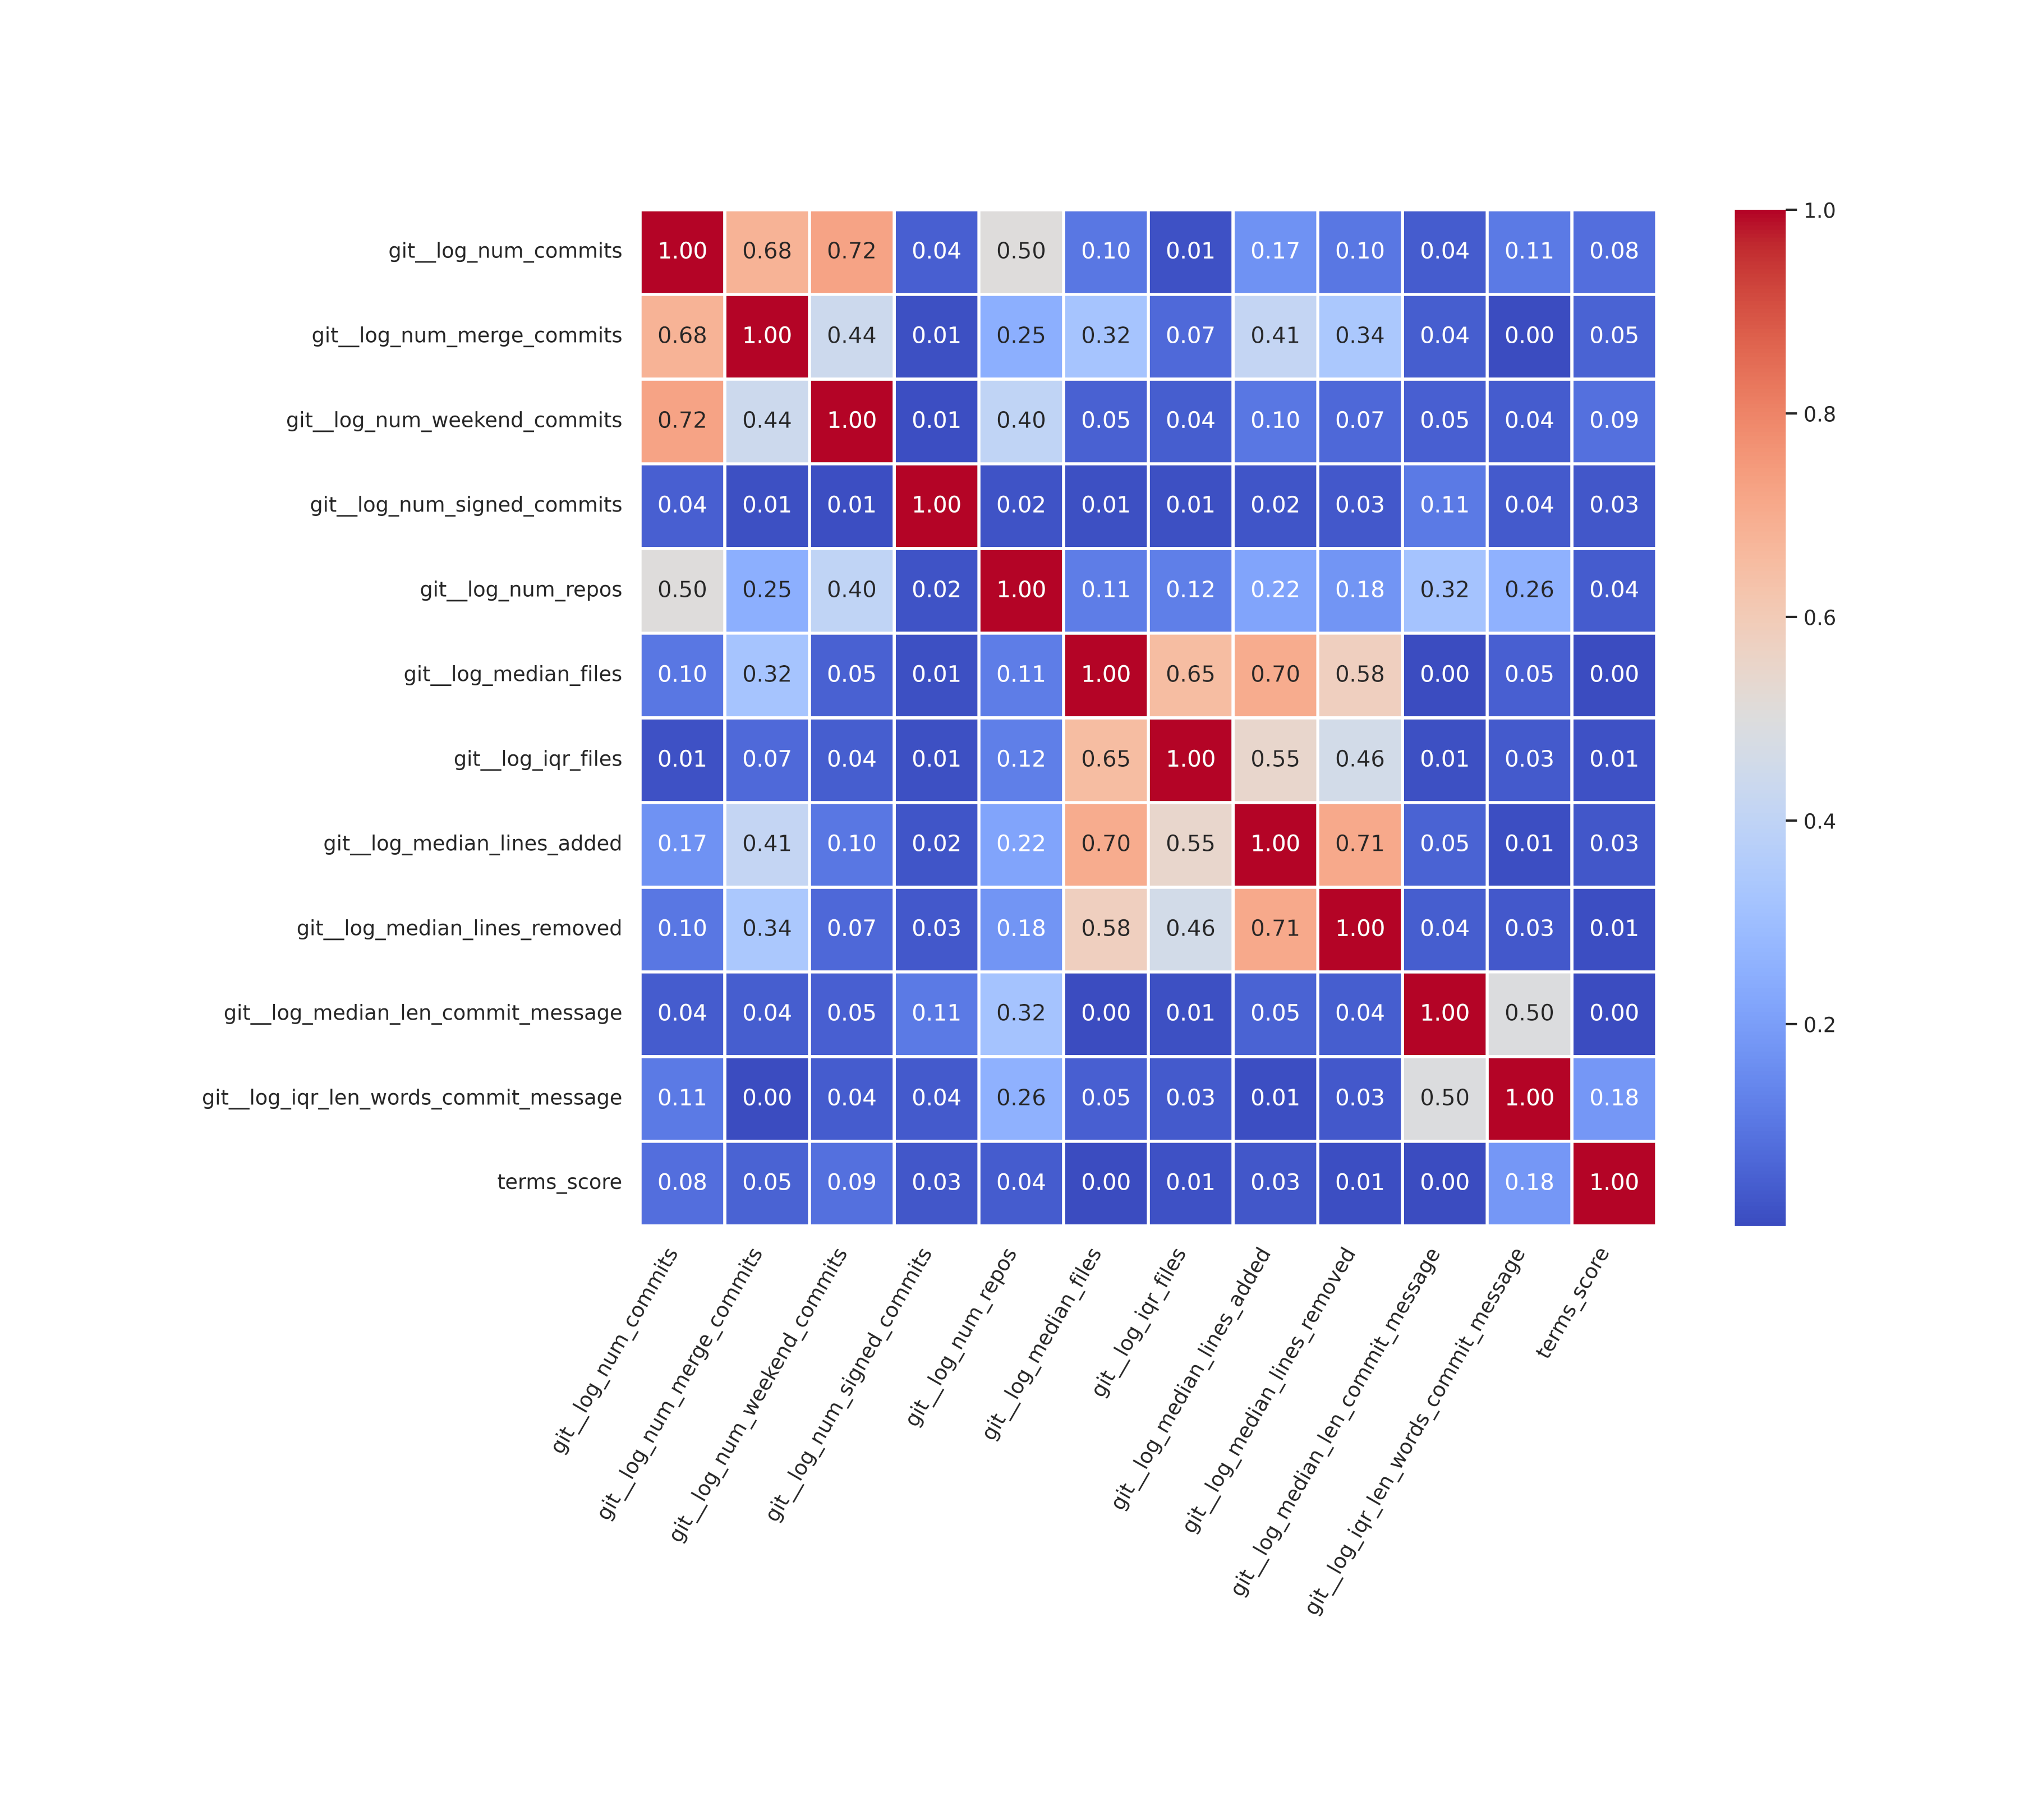
\includegraphics[width=18cm, keepaspectratio]{img/eda_corr_heatmap_correlation_fixed.png}
  \caption{Correlation heat map of the transformed variables from the training dataset.}
  \label{fig:corr-heatmap-after}
\end{figure}

\subsection{Imbalanced data}
\label{ssec:imbalanced-data}

% Interesting read: https://machinelearningmastery.com/framework-for-imbalanced-classification-projects/

We already commented in the Exploratory Data Analysis Section (\ref{ssec:eda}) on the fact that one of the main challenges of this project is the imbalance in the target class we are aiming to detect. This context was taken into account when splitting the main dataset into the training, test, and validation tests, but it needs another processing stage before they feed the different classification models. Looking at the techniques that are commonly used to reduce the effect of imbalanced data, the one selected was \textbf{SMOTE}~\cite{chawla2002smote}. 

\textit{SMOTE} consists of an algorithm generating new samples considering the k-nearest neighbours from each original sample from the \textbf{training set}. Each newly generated sample is interpolated between the original sample and one of the nearest neighbours; with a random component $\lambda$, which takes value in the range $[0, 1]$.

To apply SMOTE, we rely on the implementation under the \texttt{over\_sampling} module from the Python library \textit{imblearn} (\ref{sssec:imblearn}).

\begin{figure}
 \centering
  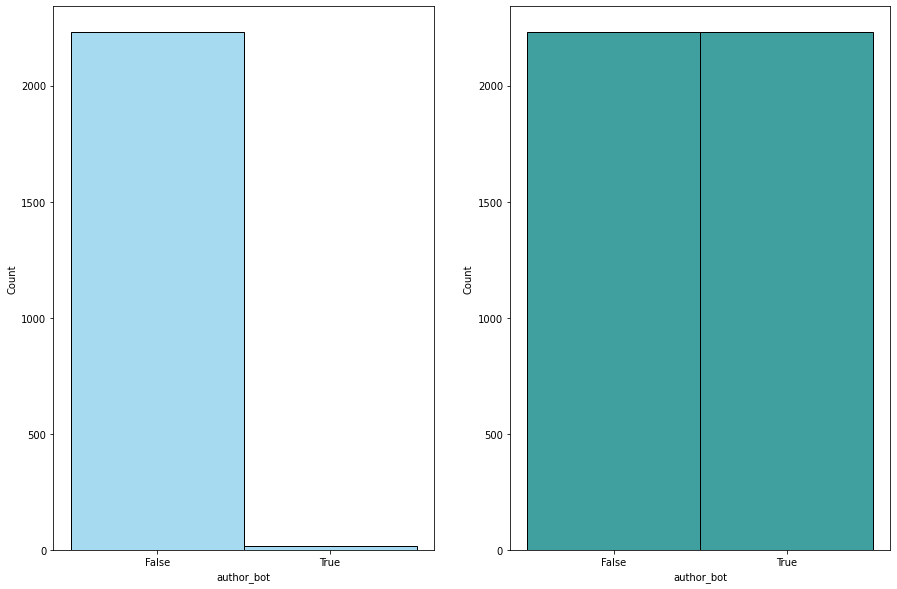
\includegraphics[width=17cm, keepaspectratio]{img/author_bot_SMOTE_train.png}
  \caption{Effect of applying SMOTE over the training dataset on the target variable; before (left) and after (right).}
  \label{fig:smote-train}
\end{figure}

\section{Classification model} 
\label{sec:classification-model}

The next step in the tool is running the classification model that allows to classify the contributors. The type of variables we have can be separated into two groups: those variables coming from the activity of each contributor and those variables we have generated from the contributors' names based on a set of heuristic terms.

The initial idea was to split the corresponding variables from these two groups into different subsets of the data, and each of the subsets would be evaluated by different classification models. Then, the output of both models can be directed to an ensemble model that would produce a final output.

\subsection{Models definition}
\label{ssec:models-definition}

In this subsection, the classification models considered for this project are explained in more depth~\footnote{The mathematical definitions are extracted from the book ``An Introduction to Statistical Learning''~\cite{introstatlearning}}. The decision was to select a set of models based on the ones used in the reference scientific papers described in Chapter~\ref{chap:state-art}. The tests and results from applying these classification models to our dataset are presented in Section~\ref{sec:exp-classification-models}.

\subsubsection{Naive-Bayes}
\label{sssec:gaussian-naive-bayes}

\textit{\textbf{Naive-Bayes}} supervised-learning algorithms are based on Bayes’ theorem. They belong to the Probability-based learning family, and their approach is to use estimations of likelihoods to determine the most likely predictions that should be made and review them later, based on the available data and also extra evidence whenever it becomes available.

\textit{Naive-Bayes} classifiers are especially useful for problems with many input variables, categorical input variables with a vast number of possible values, and text classification. Among the advantages of using these classification models are their simplicity to apply (generally, no parameters to be adjusted) and their resistance to over-fitting.

The selected classifier was the \textbf{Gaussian Naive-Bayes} algorithm implemented in Scikit-learn (\texttt{GaussianNB}\footnote{\url{https://scikit-learn.org/stable/modules/generated/sklearn.naive_bayes.GaussianNB.html}}, under \texttt{naive\_bayes} module). Mathematically, the definition for this classification model can be expressed as follows:

Being $p_{k}(x)$ the posterior probability of an observation $x$ to belong to the class $k$, which is defined as $p_{k}(x)= Pr(Y = k|X = x)$, in terms of $\pi_{1},...,\pi_{k}$ and $f_{1}(x),...,f_{k}(x)$, where $\pi_{1},...,\pi_{k}$ are the prior probabilities and $f_{1}(x),...,f_{k}(x)$ are the $p$-dimensional density functions for an observation in the $k$-th class for $k=1,...,K$; the Naive-Bayes classifier makes a single assumption for estimating $f_{1}(x),...,f_{k}(x)$ functions: Within the $k$-th class, the $p$-predictors are independent.

With this assumption, we can obtain an expression for the posterior probability,

\begin{center}
\begin{equation}
P_{r}(Y = k|X = x) = \frac{\pi_{k} \times f_{k1}(x_{1}) \times f_{k2}(x_{2}) \times ... \times f_{kp}(x_{p})}{\sum_{l=1}^{K} \pi_{l} \times f_{l1}(x_{1}) \times f_{l2}(x_{2}) \times ... \times f_{lp}(x_{p})} \quad,
\end{equation}
for $k = 1,...K$.
\end{center}

Thus, to estimate the one-dimensional density function $f_{kj}$ using training data $x_{1j},...x_{nj}$, if $X_{j}$ is quantitative we can assume that, $X_{j}|Y=k \sim N(\mu_{jk}, \sigma^2_{jk})$. In other words, we assume that within each class, the $j$th predictor is drawn for a normal distribution.

\subsubsection{Support Vector Classifier}
\label{sssec:linear-svms}

The support vector classifier is based on the possibility of constructing a
hyperplane that separates the hyperplane training observations perfectly
according to their class labels. Once this hyperplane exists, the ideal scenario
is that a test observation is assigned to a class depending on which side of
the hyperplane it is located.

Nonetheless, observations that belong to two classes are not
necessarily separable by a hyperplane. In fact, even if a \textit{separating hyperplane} does exist, then there are instances in which a classifier based on
a \textit{separating hyperplane} might not be desirable, as it will necessarily perfectly classify all of the training
observations. This can lead to sensitivity to individual observations and implies
that it may have overfitted the training data.

That is, it could be worthwhile to misclassify a few training observations
in order to do a better job discriminating the remaining observations.
The support vector classifier, sometimes called a soft margin classifier,
does exactly this. Rather than seeking the largest possible margin so that
every observation is not only on the correct side of the hyperplane but
also on the correct side of the margin, we instead allow some observations
to be on the incorrect side of the margin, or even the incorrect side of
the hyperplane.

Summarising, the support vector classifier classifies a test observation depending on
which side of a hyperplane it lies. The hyperplane is chosen to correctly
separate most of the training observations into the two classes, but may
misclassify a few observations. Taking the mathematical definition of a $p$-dimensional hyperplane, 
\begin{center}
\begin{equation}
\beta_{0} + \beta_{1}X_{1} + \beta_{2}X_{2} + ... + \beta_{p}X_{p} = 0 \quad,
\end{equation}
\end{center}
the separating hyperplane is the solution to this optimisation problem:
\begin{center}
\begin{equation}
maximize\ M (\beta_{0}, \beta_{1},...,\beta_{p}, \epsilon_{0}
,...\epsilon_{n}, M)\quad,
\end{equation}
\begin{equation}
subject\ to \sum_{j=1}^{p} \beta_{j}^2 = 1 \quad,
\end{equation}
\begin{equation}
y_{i}(\beta_{0} + \beta_{1}x_{i1} + \beta_{2}x_{i2} +...+ \beta_{p}x_{ip}) \geq M(1-\epsilon_{i}) \quad, 
\end{equation}
\begin{equation}
\epsilon_{i} \geq 0, \quad \sum_{i=1}^{n}\epsilon_{i} \leq C \quad, 
\end{equation}
\end{center}

where $C$ is a non-negative tuning parameter.

% This classifier is based on the \textit{\textbf{Support vector machine}} (SVM) are a set of supervised learning methods used for classification, regression, and outliers detection. 

% Among the advantages of using support vector machines, they are proven to be effective in high dimensional spaces, even in cases where the number of dimensions is greater than the number of samples; they are versatile, as they can use different \textit{kernel} functions for the decision; and they are memory efficient, as they use a subset of training points in the decision function (called "support vectors").

% About the disadvantages, it is important to avoid over-fitting when choosing the \textit{kernel} functions. Also, the output from these models are expensive in terms of computation load, as the probability estimates are calculated using cross-validation.

% In this case, the selected classifier was the \textbf{Linear Support Vector Classifier (SVC)} algorithm\footnote{\url{https://scikit-learn.org/stable/modules/generated/sklearn.svm.LinearSVC.html}} implemented in Scikit-learn (\texttt{LinearSVC}, under \texttt{svm} module). This method applies a linear kernel function to perform classification, by taking this linear function to find an approximated hyperplane to use it as a threshold to differentiate the classes we aim to detect. The mathematical formula is:


% \begin{center}
% \begin{equation}
% \min_ {w, b} \frac{1}{2} w^T w + C \sum_{i=1}^{n}\max(0, 1 - y_i (w^T \phi(x_i) + b)) \quad ,
% \end{equation}
% \end{center}

% where $\phi$  is the identity function.

\subsubsection{K-Nearest Neighbours}
\label{sssec:knn}

\textbf{\textit{K-Nearest Neighbours}} is a similarity-based classification model whose main idea is to compute the classification from a simple majority vote of the nearest neighbours of each point: a query point is assigned the data class which has the most representatives within the nearest $k$ (integer number) neighbours of the point.

Note that this algorithm uses the whole training dataset for making the predictions, and aside from other classification models, there are no specific assumptions that should be made concerning the data. One of the main setbacks is the fact that this algorithm is affected by noise, which implies this parameter $k$ needs to be selected carefully, particularly when working with imbalanced datasets.

This model can be found as \texttt{KNeighboursClassifier}\footnote{\url{https://scikit-learn.org/stable/modules/generated/sklearn.neighbors.KNeighborsClassifier.html}} in Scikit-learn, under \texttt{neighbours} module).

Mathematically, this classifier can be defined as follows: Given a positive integer $K$ and a test observation $x_{0}$, the KNN classifier first identifies the neighbours $K$ points in the training data that are closest to $x_{0}$, represented by $N_{0}$. It then estimates the conditional probability for class $j$ as the fraction of points in $N_{0}$ whose response values equal $j$:

\begin{center}
\begin{equation} \label{eq:knn-proba}
P_{r}(Y = j | X = x_{0})= \frac{1}{K} \sum_{i \in N_{0}}^{} I(y_{i} = j)
 \quad.
\end{equation}
\end{center}

Finally, KNN classifies the test observation $x_{0}$ to the class with the largest probability from equation~\ref{eq:knn-proba}.

\subsubsection{Decision Tree / Random Forests}
\label{sssec:decision-trees}

% \begingroup
% \leftskip 30pt
% \rightskip 0pt plus 1fill
% \vspace{8pt}

As explained in \textit{Scikit-learn} documentation\footnote{\url{https://scikit-learn.org/stable/modules/tree.html}}, the \textbf{\textit{Decision Trees}} (DTs) are a non-parametric supervised learning method used for classification and regression. The goal is to create a model that predicts the value of a target variable by learning simple decision rules inferred from the data features. A tree can be seen as a set of if-else decision rules.

Providing a more academic definition, a classification tree predicts that each observation belongs to the most commonly 
occurring class of training observations in the region to which it belongs.

In interpreting the results of a classification tree, we are often interested not only in the class prediction
corresponding to a particular terminal node region, but also in the class proportions among the training
observations that fall into that region.

We use recursive binary splitting to grow a classification tree. Since we plan to assign an observation
in a given region to the most commonly occurring class of training observations in that region,
the classification error rate is simply the fraction of the training observations in that region that do not
belong to the most common class:

\begin{center}
\begin{equation}
 E = 1 - \underset{k}{max}(\widehat{p}_{mk}) \quad.
\end{equation}
\end{center}


Here $\widehat{p}_{mk}$ represents the proportion of training observations in the $m$-th region that are from the $k$-th class. 
However, it turns out that classification error is not sufficiently sensitive for tree-growing,
and in practice two other measures are preferable.
The Gini index is defined by

\begin{center}
\begin{equation}
G = \sum_{k=1}^{K} \widehat{p}_{mk}(1 -  \widehat{p}_{mk}) \quad ,
\end{equation}
\end{center}

a measure of total variance across the $K$ classes. It is not hard to see that the Gini index takes on
a small value if all of the $\widehat{p}_{mk}$ ’s are close to zero or one.  For this reason the Gini index
is referred to as a measure of node \emph{purity}—a small value indicates that a node contains predominantly
observations from a single class.

An alternative to the Gini index is entropy, given by

\begin{center}
\begin{equation}
D = - \sum_{k=1}^{K} \widehat{p}_{mk}\log \widehat{p}_{mk}   \quad .
\end{equation}
\end{center}

Since $0 \leq  \widehat{p}_{mk} \leq 1$, it follows that $0 \leq - \widehat{p}_{mk} \log  \widehat{p}_{mk}$.
One can show that the entropy will take on a value near zero if the $\widehat{p}_{mk}$’s are all near zero or
near one. Therefore, like the Gini index, the entropy will take on a small value if the $m$-th node is pure.
In fact, it turns out that the Gini index and the entropy are quite similar numerically.

When building a classification tree, either the Gini index or the entropy is typically used to evaluate
the quality of a particular split, since these two approaches are more sensitive to node purity than 
the classification error rate. Any of these three approaches might be used when pruning the
tree, but the classification error rate is preferable if the prediction accuracy of the final pruned tree is the goal.

Some of the main advantages of decision trees algorithm are:
\begin{itemize}
    \item It is simple to understand and interpret. Trees can be visualised: if a given situation is observable, the explanation for the condition is easily explained by Boolean logic.
    \item Requires little data preparation. Other techniques often require data normalisation, dummy variables need to be created and blank values to be removed.
    \item Performs well even if its assumptions are somewhat violated by the true model from which the data were generated.
\end{itemize} 

The most remarkable disadvantages are:
\begin{itemize}
    \item DTs can create over-complex trees that do not generalise the data well (over-fitting).
    \item They can be unstable because small variations in the data might result in a completely different tree being generated.
    \item Decision-tree learners create biased trees if some classes dominate. In our case, this effect would be mitigated because we applied SMOTE to balance both classes.
\end{itemize}

Regarding the two first disadvantages, both can be addressed by using an ensemble model taking
many decision trees. This is where the \textbf{\textit{Random Forest}} (RF) classifier\footnote{\url{https://scikit-learn.org/stable/modules/generated/sklearn.ensemble.RandomForestClassifier.html}}
comes into play: it builds a number of decision trees on bootstrapped training samples. When building
these decision trees, each time a split in a tree is considered, a random sample of $m$ predictors is 
chosen as split candidates from the full set of $p$ predictors. The split is allowed to use only one of 
those $m$ predictors. A fresh sample of $\sqrt{m}$ predictors is taken at each split, and typically
we choose $m \approx p$—that is, the number of predictors considered at each split is approximately
equal to the square root of the total number of predictors.

Then, the prediction of the ensemble is computed as the averaged prediction of these individual 
classifiers, improving the predictive accuracy and preventing over-fitting. The implementation of this 
classifier can be found as \texttt{RandomForestClassifier} (under the \texttt{ensemble} module) 
in Scikit-learn.

\subsubsection{XGBoost Classifier}
\label{sssec:xgboost-classifier}

The XGBoost Classifier model belongs to the XGBoost library (see subsection~\ref{sssec:state-art-xgboost}). XGBoost is an ensemble model which uses decision trees as base learners. XGBoost uses CART trees (Classification and Regression trees), with scores on whether an observation belongs to a class or not. When this process reaches the max depth of the tree, the algorithm converts the scores into categories assigning a threshold value.

\subsection{Evaluation metrics}
\label{ssec:evaluation-metrics}

We need to use a set of metrics that help us to evaluate the performance of the different classification models. The main method to compare the results from the different models is a confusion matrix, which displays the number of elements that have and have not been identified correctly. The structure of this matrix is exemplified in Table~\ref{table:example-confusion-matrix}.

Looking at the possible values we can obtain, it is worth mentioning that not all the misclassified cases affect our use case in the same way: having ``False'' Negatives is worse than having ``False'' Positives. This means it is more important to classify as many bot accounts as possible (and not mistake any of them for a human) rather than classifying a human as a bot when it is not the case. In the first case, missing a bot account among the plethora of contributors in a community could mean that potentially this bot account remains hidden (and hardly going to be identified); while in the latter, this wrong recommendation could be just ignored.

This situation links directly to the definition of two basic metrics: \emph{precision} and \emph{recall}. As it is defined in Scikit-learn's documentation page\footnote{\url{https://scikit-learn.org/stable/modules/model_evaluation.html\#precision-recall-f-measure-metrics}}, an intuitive definition of precision is the ability of the classifier not to label as positive a sample that is negative, and recall is the ability of the classifier to find all the positive samples.

Precision is defined mathematically as:

\begin{center}
\begin{equation}
Precision = \frac{tp}{tp+fp} \quad,
\end{equation}
\end{center}

and recall is defined as: 

\begin{center}
\begin{equation}
Recall = \frac{tp}{tp+fn} \quad.
\end{equation}
\end{center}

Although it is common to use the \emph{F1-score} as an evaluation metric for classification models, this score is considering that the recall and the precision are equally important. This is why the decision was to use a \emph{$F_{\beta}$} score with $\beta = 2$, to penalise those classification models with a greater number of ``False'' Negatives.

\begin{table}[tb]
\renewcommand{\arraystretch}{1.5}
\begin{center}
%\begin{tabular}{ l | r c c }
\begin{tabular}{ l r c c }
\toprule
%\rowcolor[HTML]{C0C0C0}
      &                & \multicolumn{2}{c}{Predicted} \tabularnewline
      %\midrule
      &                & \textbf{Human}                              & \textbf{Bot} \\
                         
 Real & \textbf{Human} & \cellcolor[HTML]{67FD9A}True Negative (TN)  & \cellcolor[HTML]{FD6864}False Positive (FP) \\ %\hline
      & \textbf{Bot}   & \cellcolor[HTML]{FD6864}False Negative (FN) & \cellcolor[HTML]{67FD9A}True Positive (TP) \\ %\hline
\bottomrule
\end{tabular}
\caption{Example of confusion matrix to evaluate the classifiers' performance.}
\label{table:example-confusion-matrix}
\end{center}
\end{table}

\cleardoublepage

%%%%%%%%%%%%%%%%%%%%%%%%%%%%%%%%%%%%%%%%%%%%%%%%%%%%%%%%%%%%%%%%%%%%%%%%%%%%%%%%
%%%%%%%%%%%%%%%%%%%%%%%%%%%%%%%%%%%%%%%%%%%%%%%%%%%%%%%%%%%%%%%%%%%%%%%%%%%%%%%%
% EXPERIMENTOS Y VALIDACIÓN %
%%%%%%%%%%%%%%%%%%%%%%%%%%%%%%%%%%%%%%%%%%%%%%%%%%%%%%%%%%%%%%%%%%%%%%%%%%%%%%%%

\chapter{Experiments and validation}
\label{chap:experiments}

In this chapter, the different experiments that were run over the different phases of the project are explained. Although the main experiments are those belonging to the testing and adjustment of the classification models, there were some efforts during the data processing that are worth mentioning.

\section{Data processing: Analysing text}
\label{sec:exp-text-richness}

The following questions were proposed at the Specific objectives Section (\ref{ssec:specific-objectives}): 
\begin{itemize}
    \item \textbf{Q2.2.} Can the message content (commit messages, issue texts, etc.) be used to validate this classification?
    \begin{itemize}
        \item \textbf{Q2.2.1.} Does a richer syntax give a hint about the nature of the user? 
        \item \textbf{Q2.2.2.} Can the entropy of a comment give a hint about the nature of the user?
    \end{itemize}
\end{itemize}

Given that the initial dataset contains the history of commit messages for each user, the goal was to obtain a single, summary metric from these commit messages; so we can compare the results among the different users.

The main hypothesis from where this experiment starts is that it would be expected for bot users to have less dissimilarity among their commit messages than human users. Thus, in order to compare these comments from a given user, we decided to use a distance metric: the \textbf{Levenshtein distance} (\ref{sec:levenshtein-definition}). Then, we would obtain distance matrices, so we could observe some properties, such as if the matrices are dense or sparse with respect to the average, for instance.

As this distance had to be computed per every single pair of messages, the result was a series of symmetric matrices, where the value from each position \textit{(i, j)} was the Levenshtein distance from the message \textit{i} to the message \textit{j}; except from the main diagonal, whose values were $0$ (there is no distance from one message to itself). This computation was largely costly, as the number of calculations per user is:

\begin{center}
    \begin{equation}
    \mathrm{NumCalculations} = \frac{( NumMessages )^2}{2} \quad.
    \end{equation}
\end{center}

The decision to reduce the computation time was to limit the number of commit messages per user up to $1,500$, selected randomly. This decision entails many problems, such as the temporal dependence of these commit messages. To avoid it, some main solutions were considered: one was to get the most recent commit messages, given the nature of the data, and the other one was to get a stratified sample by a given time period (months, years, etc.).

Aside from these complications, the next problem was to compare all these matrices by finding one metric capable of summarising the information from the matrix of distances. After exploring some options and reading some literature, an idea was to compute the \textit{Mahalanobis distance} (\ref{sec:mahalanobis-definition}) between two matrices, taking into account that this distance is computed between two statistical distributions. Once computed, we would end up with a new feature characterising the set of values. When trying to compute the Mahalanobis distance between matrices, we encountered another problem. The algorithm computing this distance included, among its steps, computing the inverse matrix. It turned out some of the obtained matrices were singular (they had no inverse matrix). This last setback, together with the rest of the problems we encountered, was increasing too much the complexity of the experiment, so we decided not to continue further with it.

\section{Choosing the classification model} 
\label{sec:exp-classification-models}
% \textbf{Atención}: Este capítulo se introdujo como requisito en 2019.

% Describe los experimentos y casos de test que tuviste que implementar para validar tus resultados. 
% Incluye también los resultados de validación que permiten afirmar que tus resultados son correctos.

\begin{figure}
 \centering
  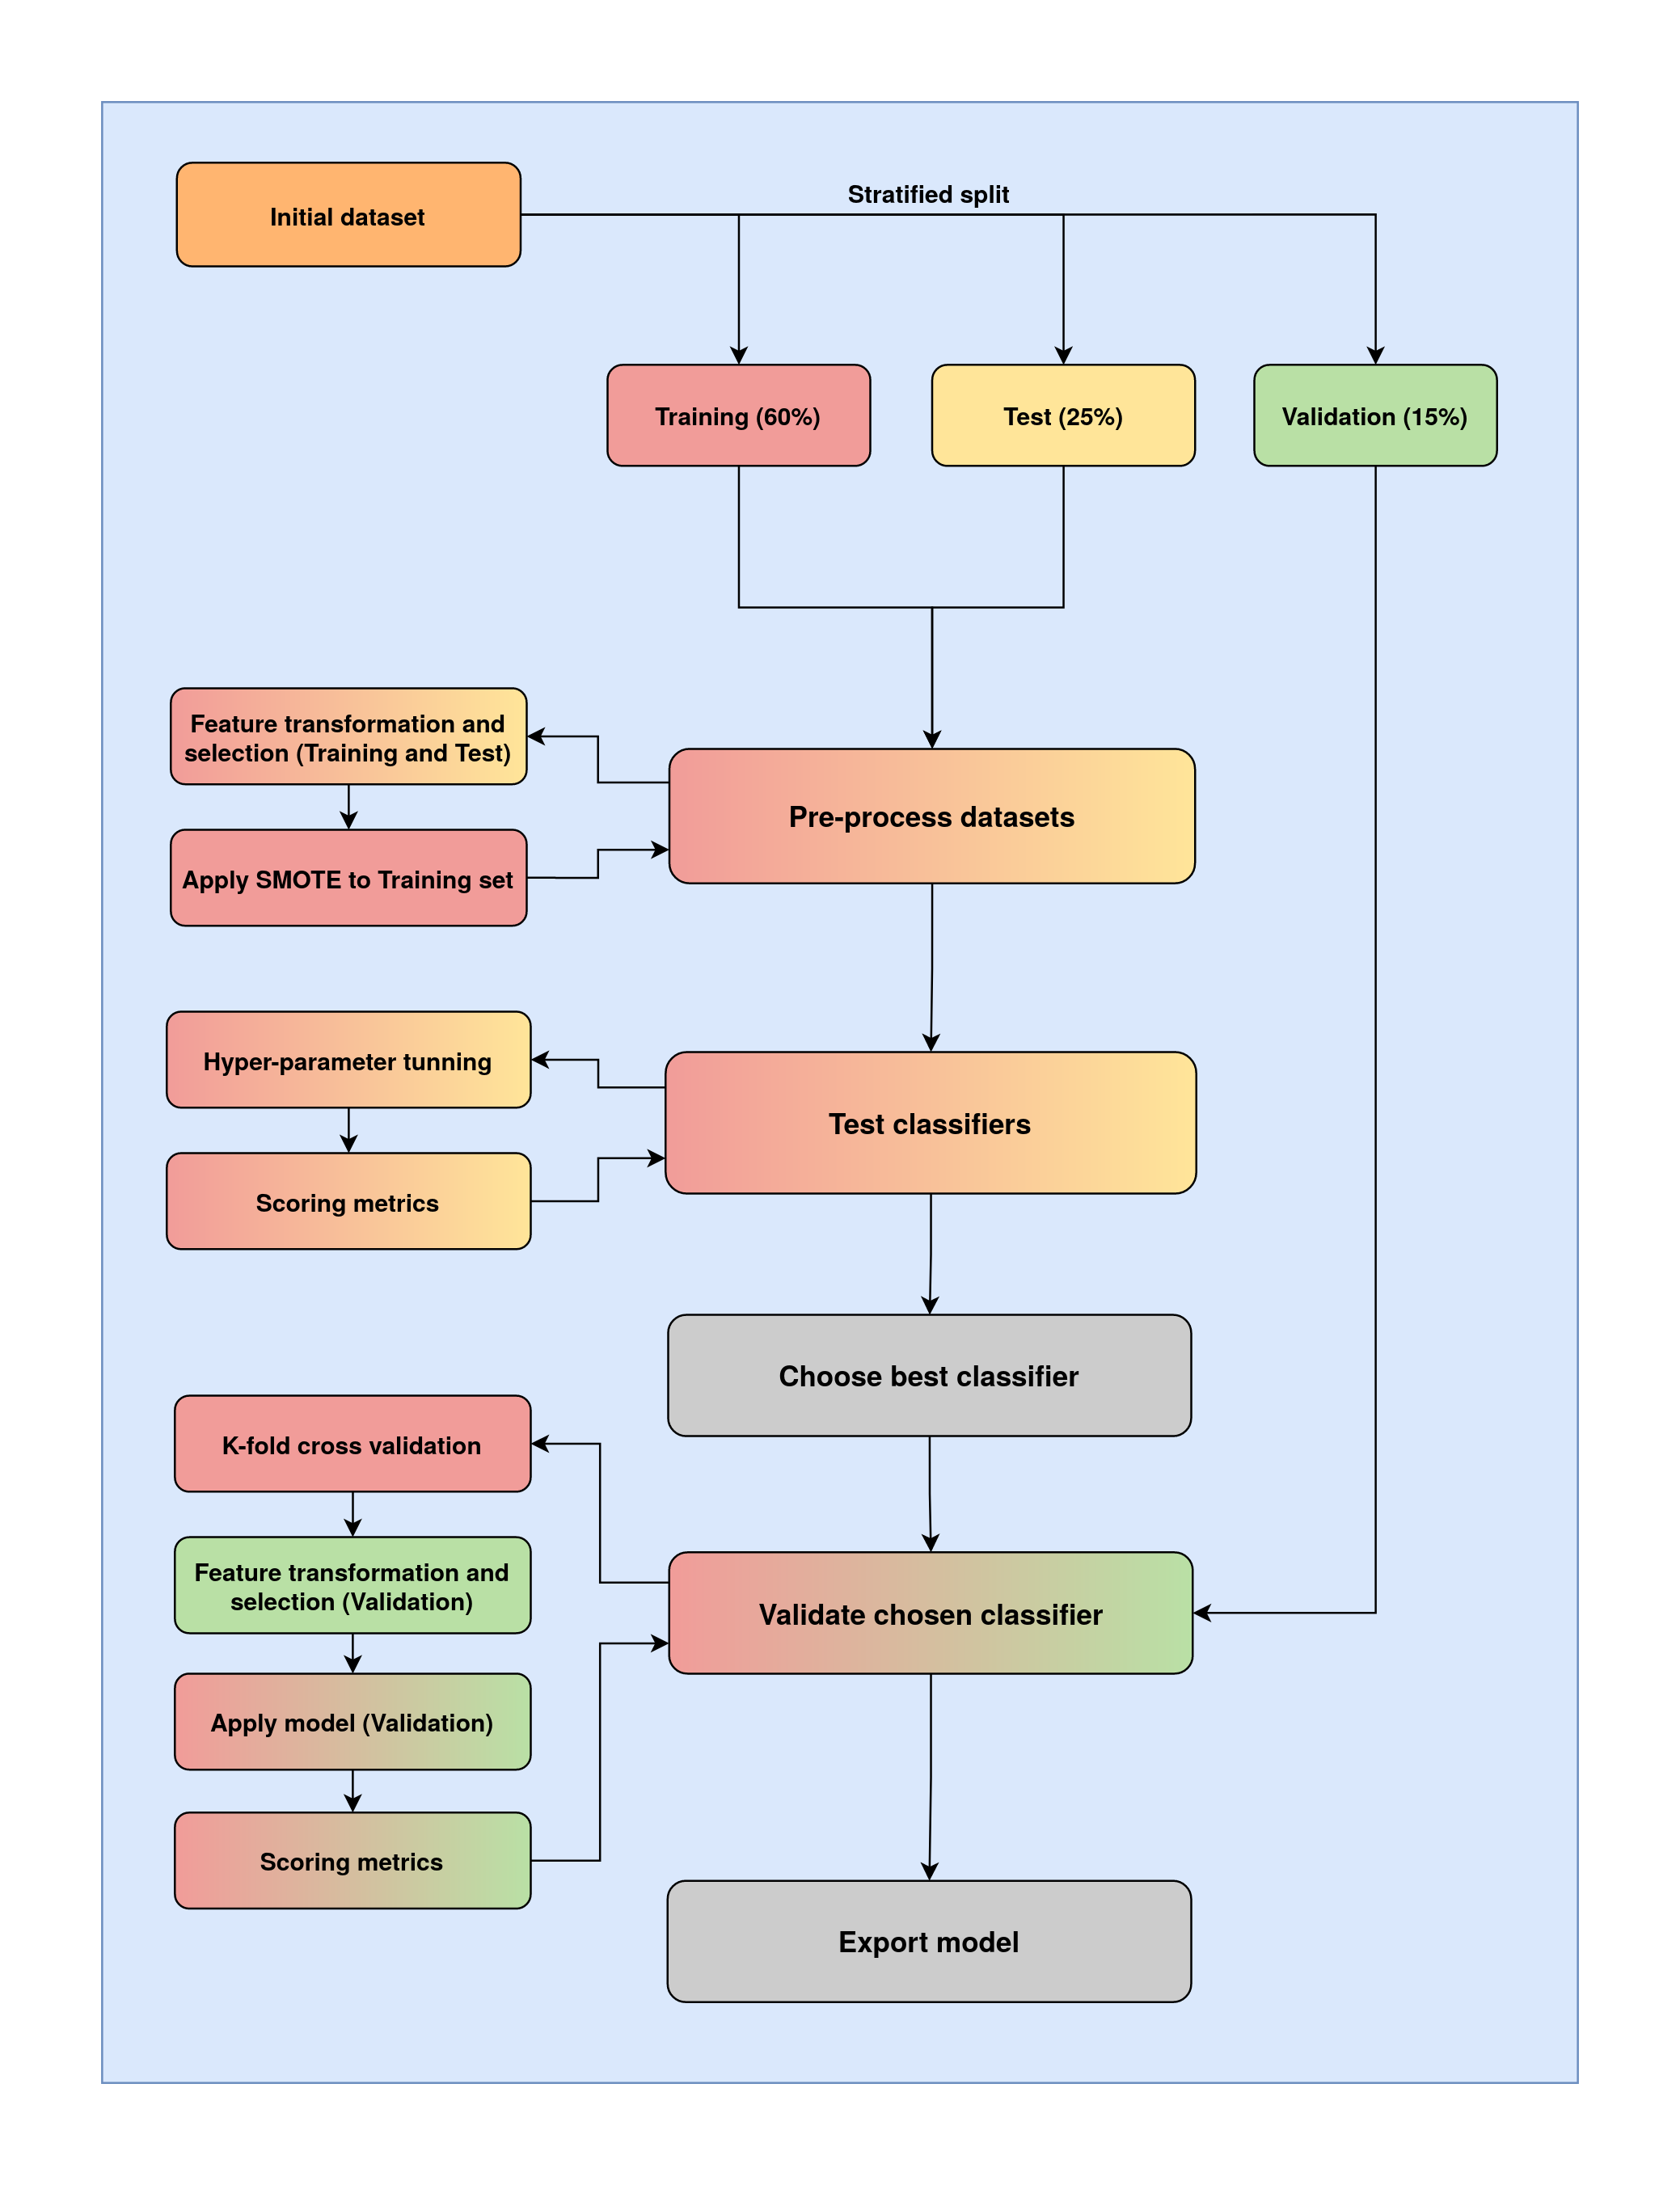
\includegraphics[width=16cm, keepaspectratio]{img/process-classification-models.png}
  \caption{Description of the classification process. Background colours for each box explain which datasets (Training, Test and Validation) are involved in each step.}
  \label{fig:model-classification-process}
\end{figure}

In this phase of the experiment process, the goal is to train the classification models we defined (\ref{ssec:models-definition}) and test their performance against our dataset. Then, after having the results using the proposed evaluation metrics (\ref{ssec:evaluation-metrics}) we will choose the best classifier. This whole process is detailed in Figure~\ref{fig:model-classification-process}, and it starts with the splitting of our initial dataset into three sets (Training, Test, and Validation), following the criteria we discussed at subsection~\ref{ssec:build-training-datasets} and then apply the pre-processing step: the transformation and selection of features (over the Training and Test datasets) and also applying SMOTE to mitigate the effect of the imbalance of the classes.

At this point, the decision was to show how the samples from the Training set were distributed using the t-SNE algorithm, a nonlinear dimensionality reduction technique~\cite{vandermaaten-et-at:t-sne08}. This way we could convert our high-dimensional dataset into a two-dimensional one, preserving the distance between the samples in the new dimensional space. In Figures~\ref{fig:data-tsne} and~\ref{fig:data-tsne-smote} we can observe the resized Training dataset before and after applying SMOTE, respectively: In the first image (Figure~\ref{fig:data-tsne}), we can observe very few occurrences of positive bot accounts, and heavily mixed among the rest of the samples from the other class; while in the second image (Figure~\ref{fig:data-tsne-smote}) we can observe a much clearer distinction between the two classes, after the synthetic samples generated by SMOTE. Apart from the interesting pattern these samples are forming, we infer that there should be a classification model capable of separating both classes.

\begin{figure}
 \centering
  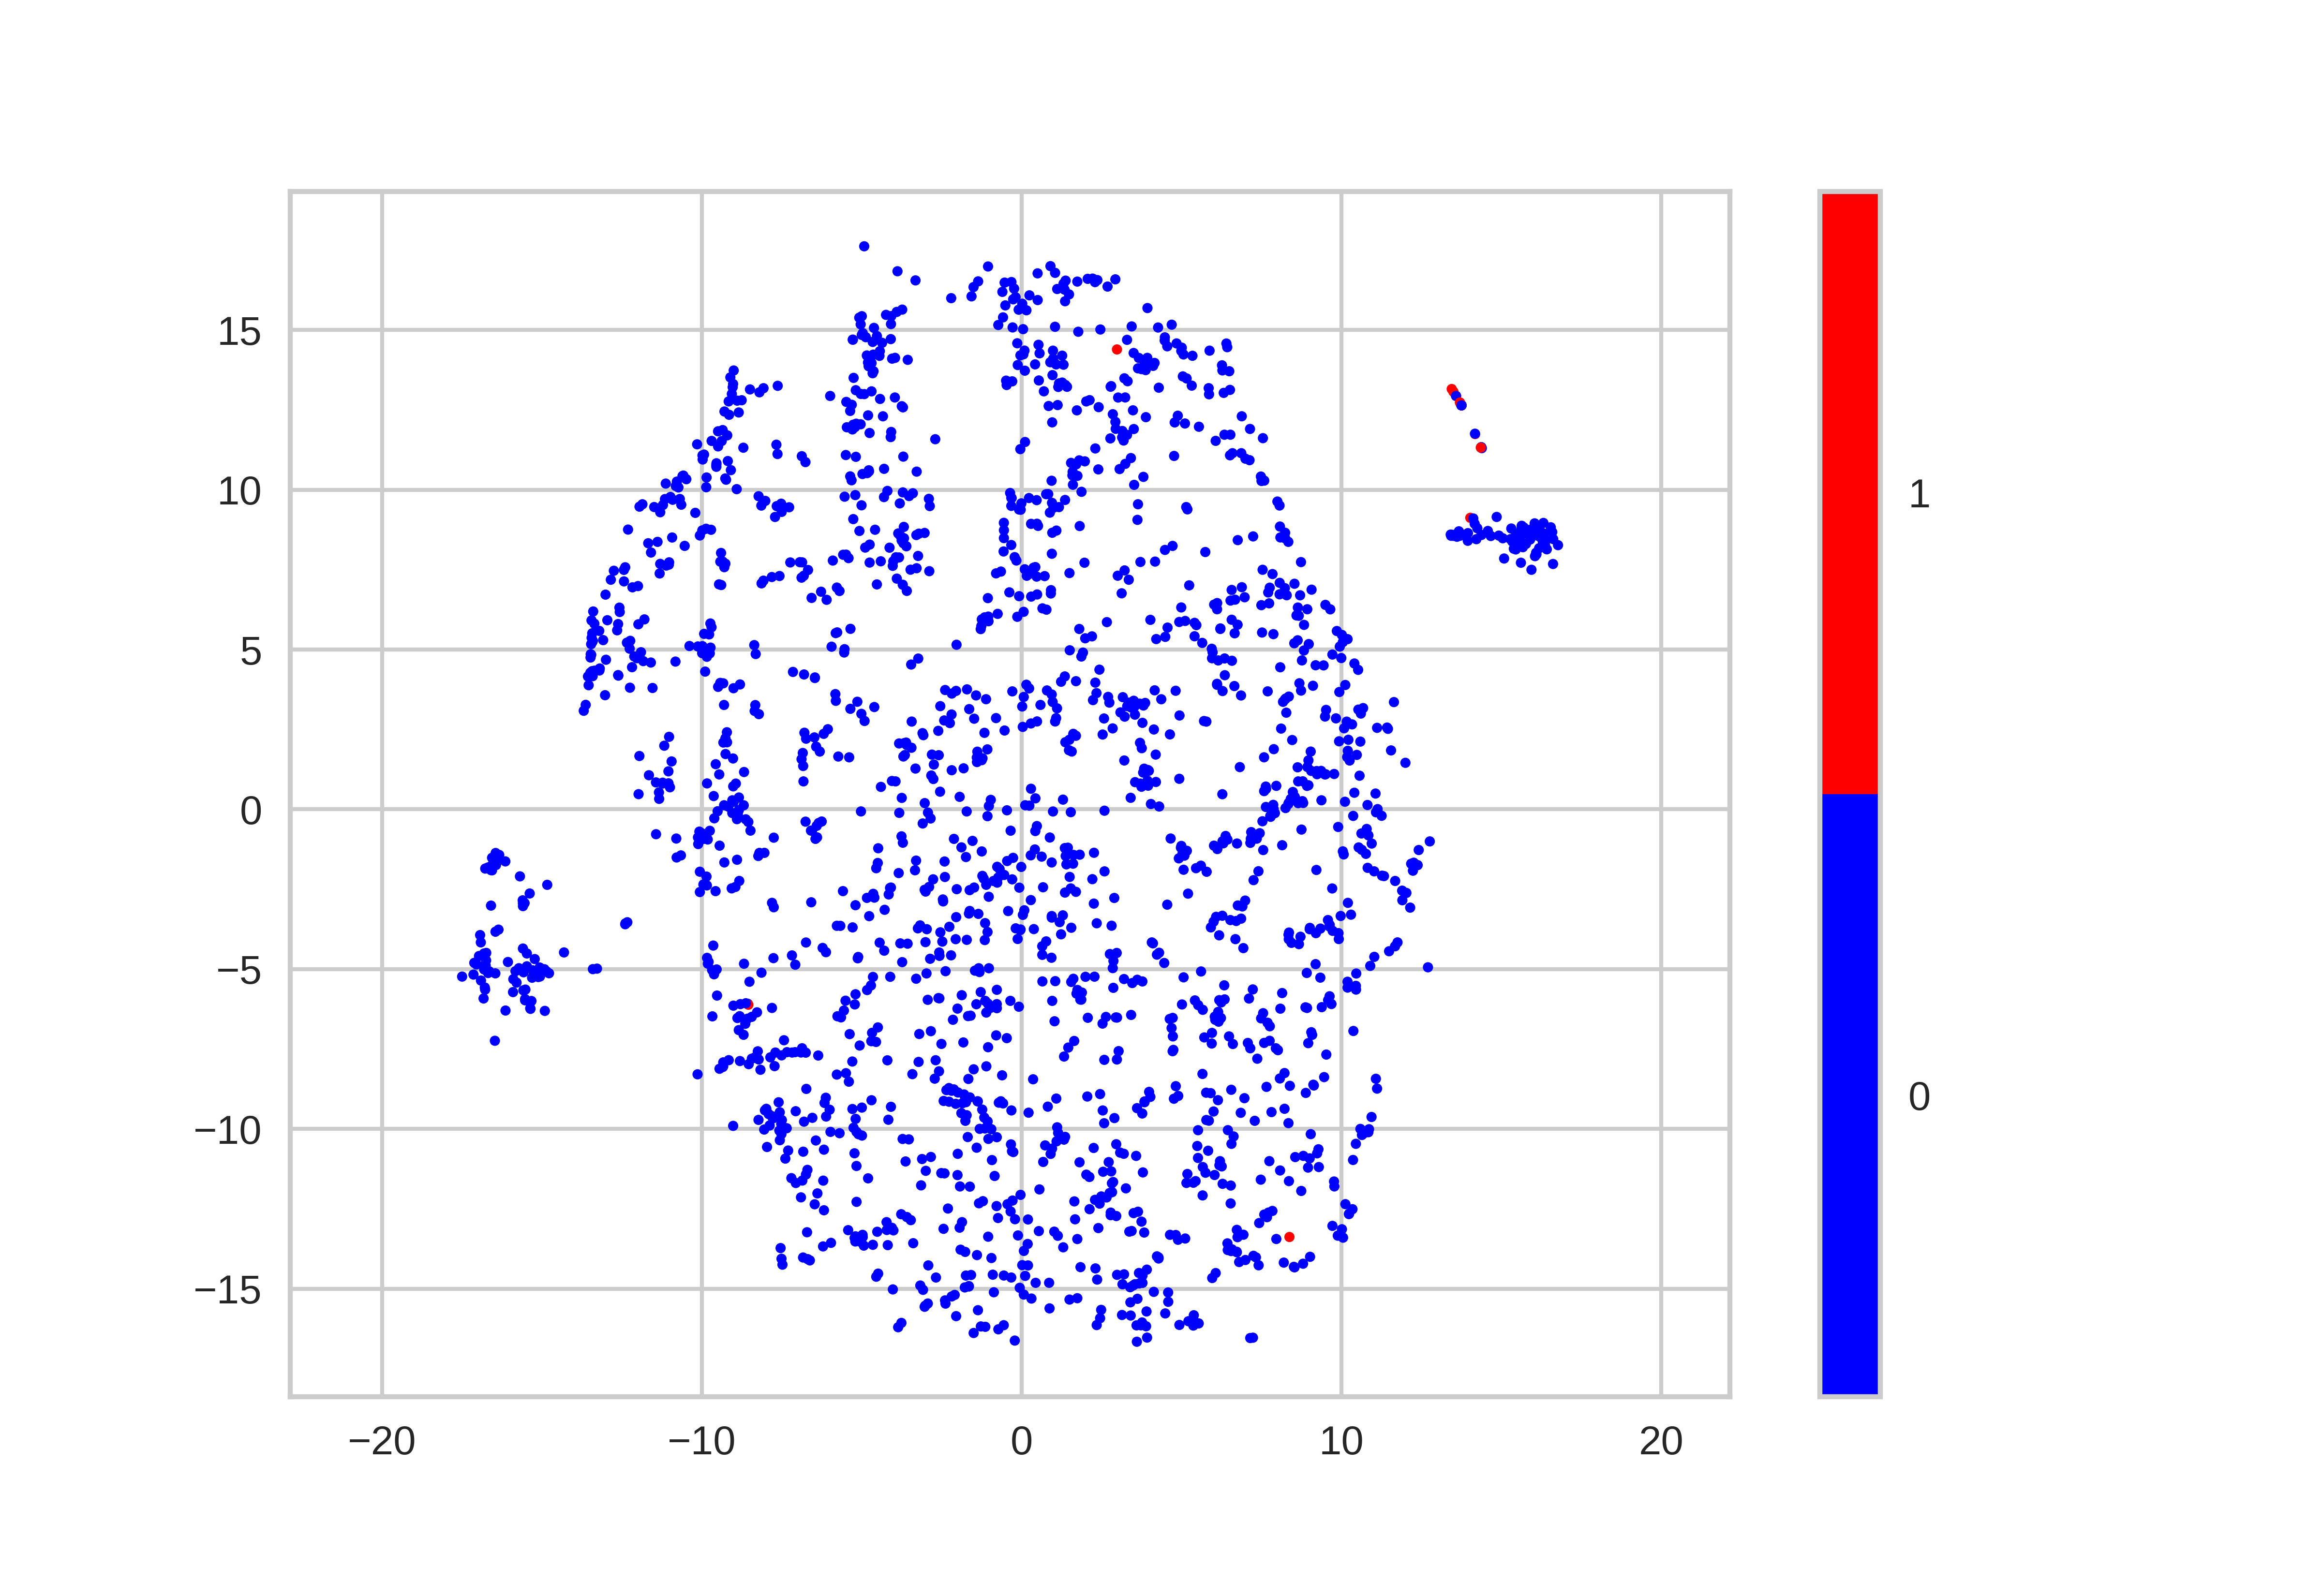
\includegraphics[width=15cm, keepaspectratio]{img/data-tsne.png}
  \caption{Visualising the Training dataset with t-SNE (Blue ($0$): Human, Red ($1$): Bot).}
  \label{fig:data-tsne}
\end{figure}

\begin{figure}
 \centering
  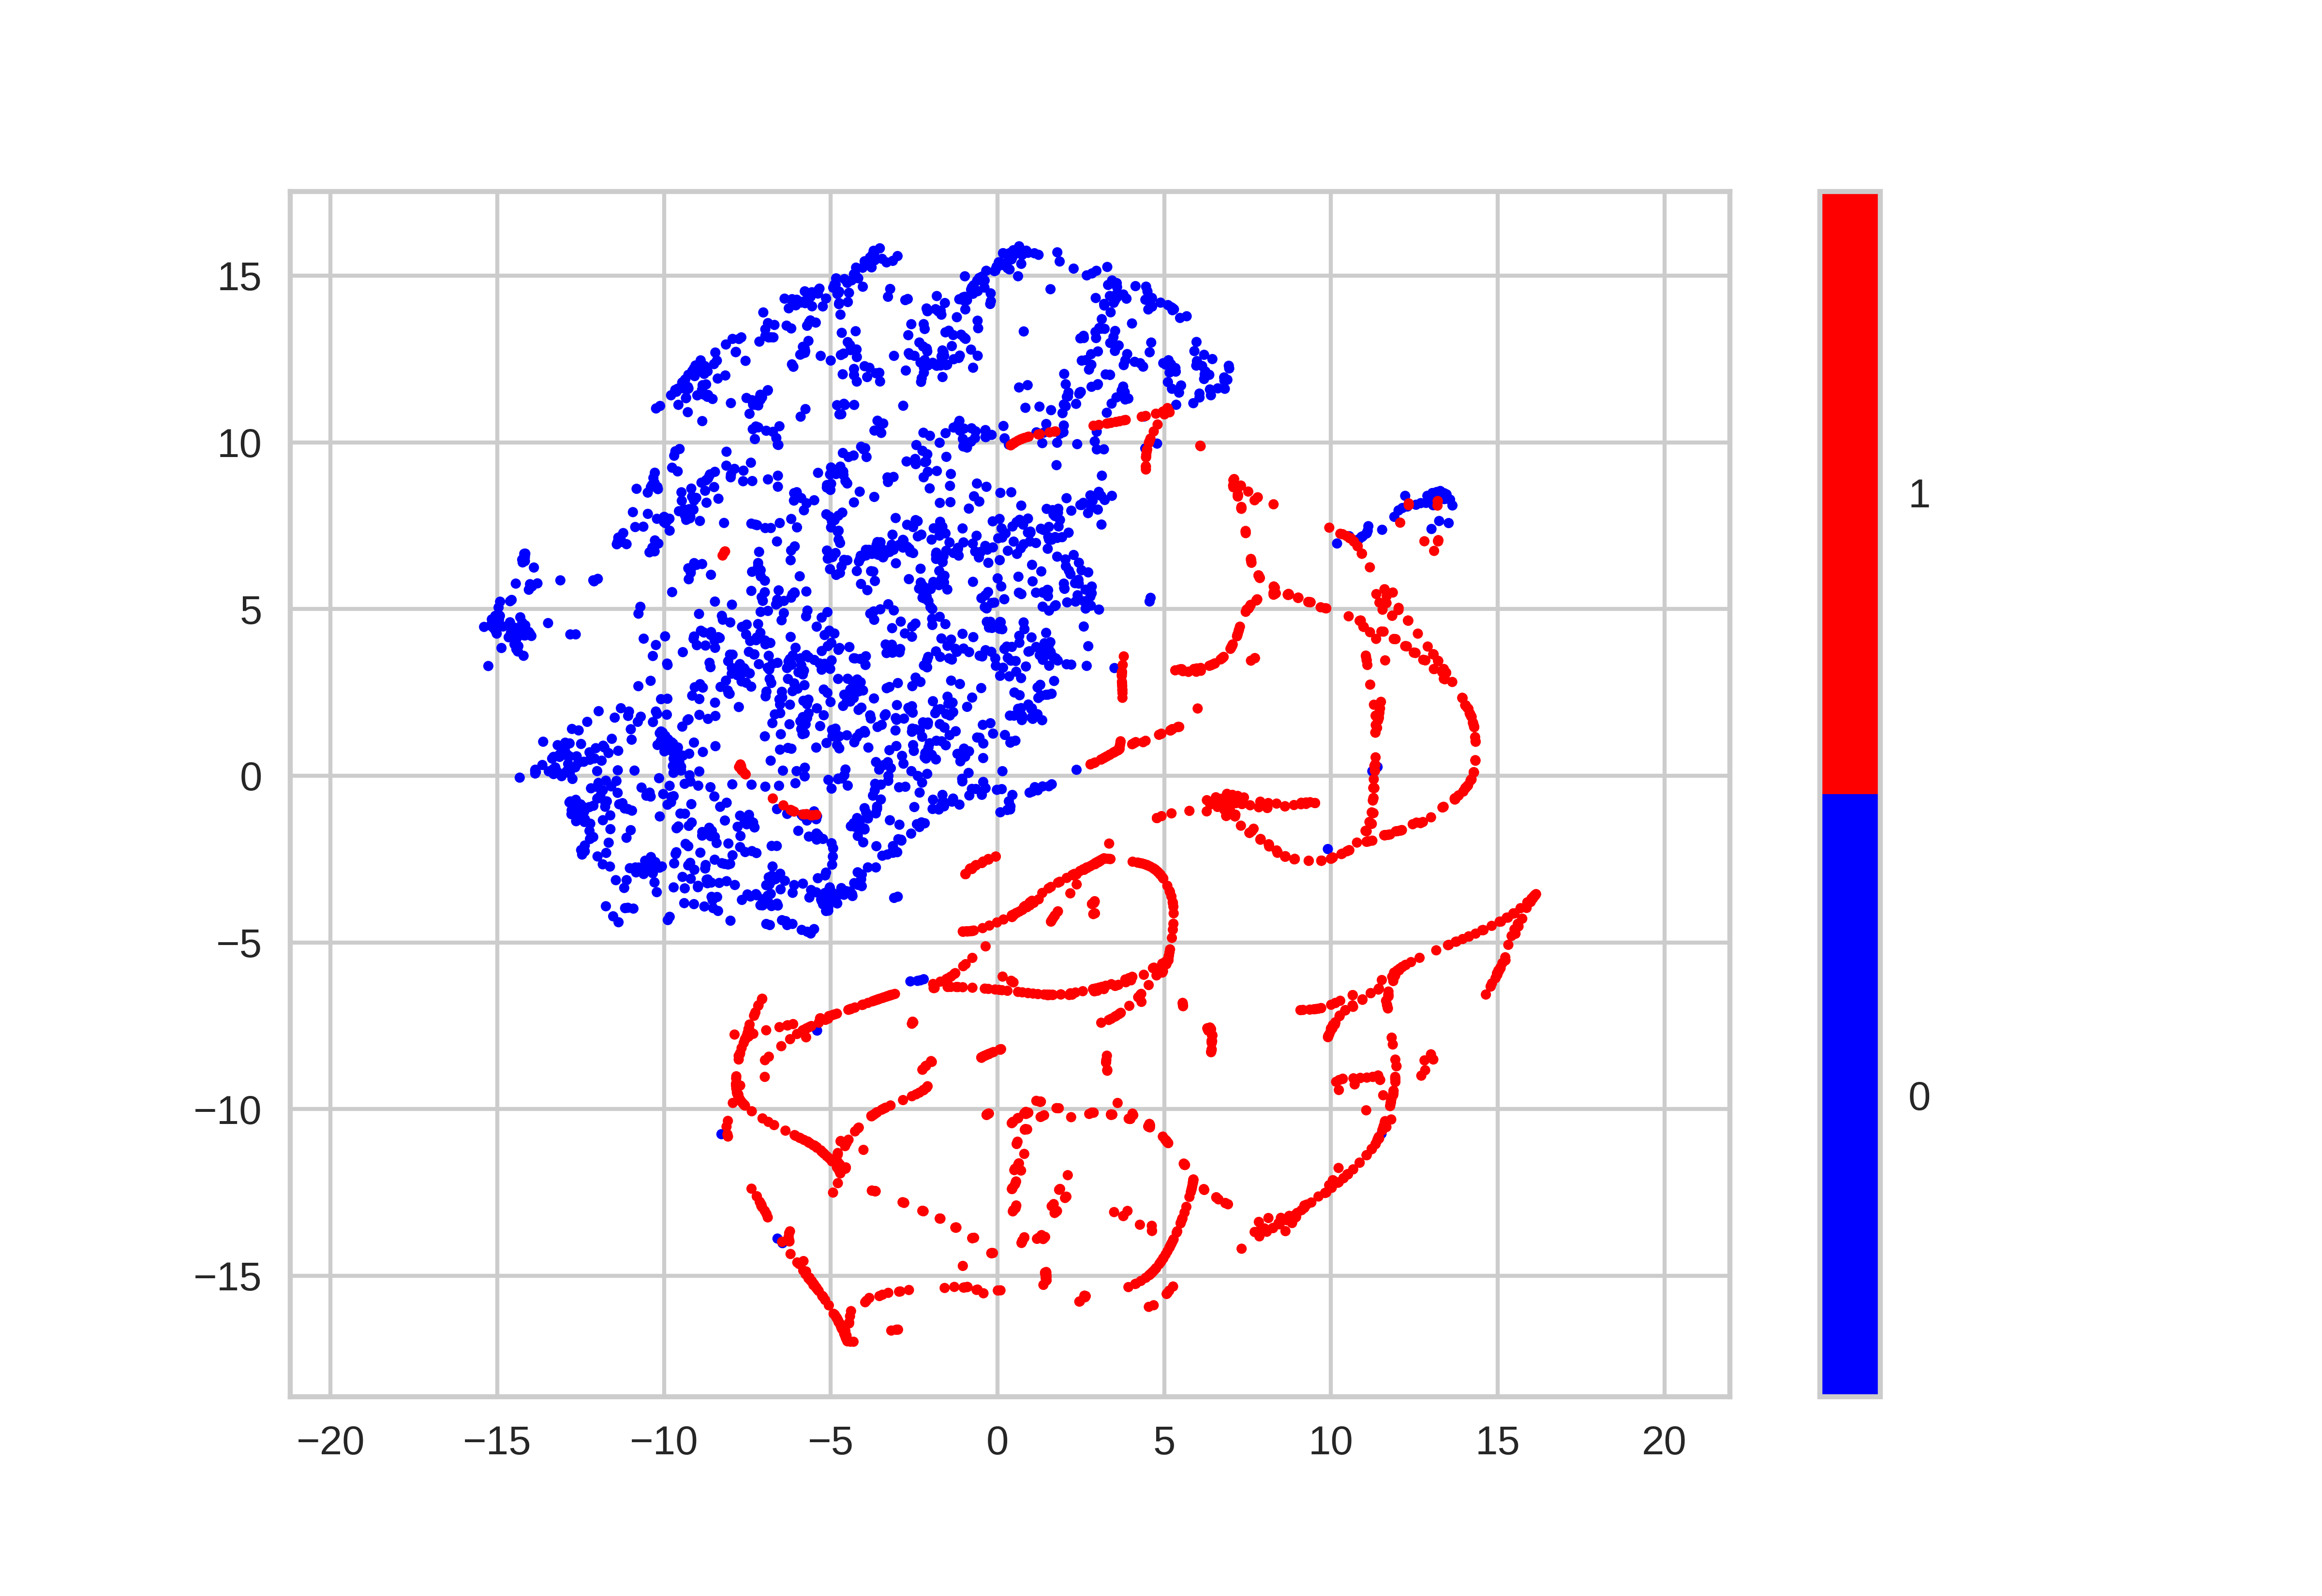
\includegraphics[width=15cm, keepaspectratio]{img/data-tsne-smote.png}
  \caption{Visualising the Training dataset with t-SNE after applying SMOTE (Blue ($0$): Human, Red ($1$): Bot).}
  \label{fig:data-tsne-smote}
\end{figure}

The proposed classifiers were trained and then tested, adjusting the specific hyper-parameters for each model until finding the best scoring (see subsection~\ref{ssec:evaluation-metrics}) for each of them. Furthermore, we applied PCA\footnote{Principal Component Analysis} to discover if there was a combination of features that would suit as input for the classification model, but we discarded it as the results indicated that one component accumulated most of the percentage of variance explained.

The results from the tested classifiers are summarised in Table~\ref{table:model-results}. The classification model with the best results was the Random Forest Classifier, with \textbf{$F_{\beta} = 0.811$} using the \textbf{Test dataset}. According to the corresponding confusion matrix (\ref{table:confusion-matrix-test}), $6$ out of $7$ bot accounts were properly classified, and $826$ human accounts out of $829$. The Precision-Recall curves for the Test and Validation sets can be observed in Figures~\ref{fig:prec-rec-test} and~\ref{fig:prec-rec-val}, respectively. These results were also tested using a \textit{5-fold} cross validation.

The parameters that worked best for the Random Forest Classifier were:
\begin{itemize}
    \item Number of estimators (Trees in the forest): $300$.
    \item Split criterion: Gini impurity.
    \item Maximum depth: $4$ levels.
\end{itemize}

\newpage
When trying these results with the \textbf{Validation dataset}, the obtained score was \textbf{$F_{\beta} = 0.6$}, obtaining the classification values displayed in Table~\ref{table:model-results-val} and in the corresponding confusion matrix (\ref{table:confusion-matrix-val}), given that there were only $4$ occurrences of bot accounts, three of them were classified correctly and only one was not. Regarding the human accounts, $493$ out of $499$ accounts were classified accurately.

Looking at feature importance values (see Figure~\ref{fig:rf-feature-importance}) obtained from our chosen classifier, it is clear that the terms score variable we produced was the most relevant for deciding the classes, followed by the logarithmic transformation of the interquartile range of the number of words in the commit messages, with a relative importance of $60\%$. Then, the logarithmic transformation of the median number of files and the number of commits have a relative importance of around $20\%$, while the rest of the variables are barely significant for the classification.

\begin{table}[tb]
\renewcommand{\arraystretch}{1.5}
\begin{center}
\begin{tabular}{ l c c r }
  \toprule
  \textbf{Model name}    &  \textbf{Precision}  & \textbf{Recall}   &    \textbf{$F_{\beta}$ score} \\
    %\midrule
      Gaussian Naive-Bayes   & $0.136$  & $ 0.857$  &    $0.417$   \\ 
      Complement Naive-Bayes & $0.167$  &  $0.857$  &    $0.469$   \\  
      LinearSVC              & $0.143$  & $0.857$  &   $0.429$   \\ 
      KNN                    & $0.316$  &  $0.857$  &    $0.638$   \\ 
      Decision Tree          & $0.385$  &  $0.714$  &    $0.61$    \\  
      \rowcolor[HTML]{67FD9A} 
      Random Forest          & $0.667$  &  $0.857$  &    $0.811$   \\  
      XGBoost                & $0.444$  &  $0.571$  &    $0.541$   \\ 
  \bottomrule
\end{tabular}
\caption{Results of the different classifiers showing the most relevant scores. The coloured row indicates the model with best overall results over the Test dataset.}
\label{table:model-results}
\end{center}
\end{table}

\begin{table}[tb]
\renewcommand{\arraystretch}{1.5}
\begin{center}
\begin{tabular}{ l c c r }
  \toprule
  \textbf{Model name}    &  \textbf{Precision}  & \textbf{Recall}   &    \textbf{$F_{\beta}$ score} \\
    %\midrule
      Random Forest   & $0.333$  &  $0.75$  &  $0.6$  \\  
  \bottomrule
\end{tabular}
\caption{Results of applying the chosen classifier to the Validation dataset.}
\label{table:model-results-val}
\end{center}
\end{table}

\begin{table}[tb]
\renewcommand{\arraystretch}{1.5}
\begin{center}
%\begin{tabular}{ l | r c c }
\begin{tabular}{ l r c c }
\toprule
%\rowcolor[HTML]{C0C0C0}
      &                & \multicolumn{2}{c}{Predicted} \tabularnewline
      %\midrule
      &                & \textbf{Human}              & \textbf{Bot} \\
                         
 Real & \textbf{Human} & \cellcolor[HTML]{67FD9A} $826$ & \cellcolor[HTML]{FD6864} $3$ \\ %\hline
      & \textbf{Bot}   & \cellcolor[HTML]{FD6864} $1$   & \cellcolor[HTML]{67FD9A} $6$  \\ %\hline
\bottomrule
\end{tabular}
\caption{Confusion matrix of the results with the test dataset ($F_{\beta} = 0.811$). The green-coloured cells represent the cases where the predicted and the real value match; the red-coloured ones represent the cases where the predicted values did not match the real ones.}
\label{table:confusion-matrix-test}
\end{center}
\end{table}

\begin{table}[tb]
\renewcommand{\arraystretch}{1.5}
\begin{center}
\begin{tabular}{ l r c c }
\toprule
%\rowcolor[HTML]{C0C0C0}
      &                & \multicolumn{2}{c}{Predicted} \tabularnewline
      %\midrule
      &                & \textbf{Human}              & \textbf{Bot} \\
                         
 Real & \textbf{Human} & \cellcolor[HTML]{67FD9A} $493$ & \cellcolor[HTML]{FD6864} $6$ \\ %\hline
      & \textbf{Bot}   & \cellcolor[HTML]{FD6864} $1$   & \cellcolor[HTML]{67FD9A} $3$  \\ %\hline
\bottomrule
\end{tabular}
\caption{Confusion matrix of the results with the validation dataset ($F_{\beta} = 0.6$). The green-coloured cells represent the cases where the predicted and the real value match; the red-coloured ones represent the cases where the predicted values did not match the real ones.}
\label{table:confusion-matrix-val}
\end{center}
\end{table}


\begin{figure}
 \centering
  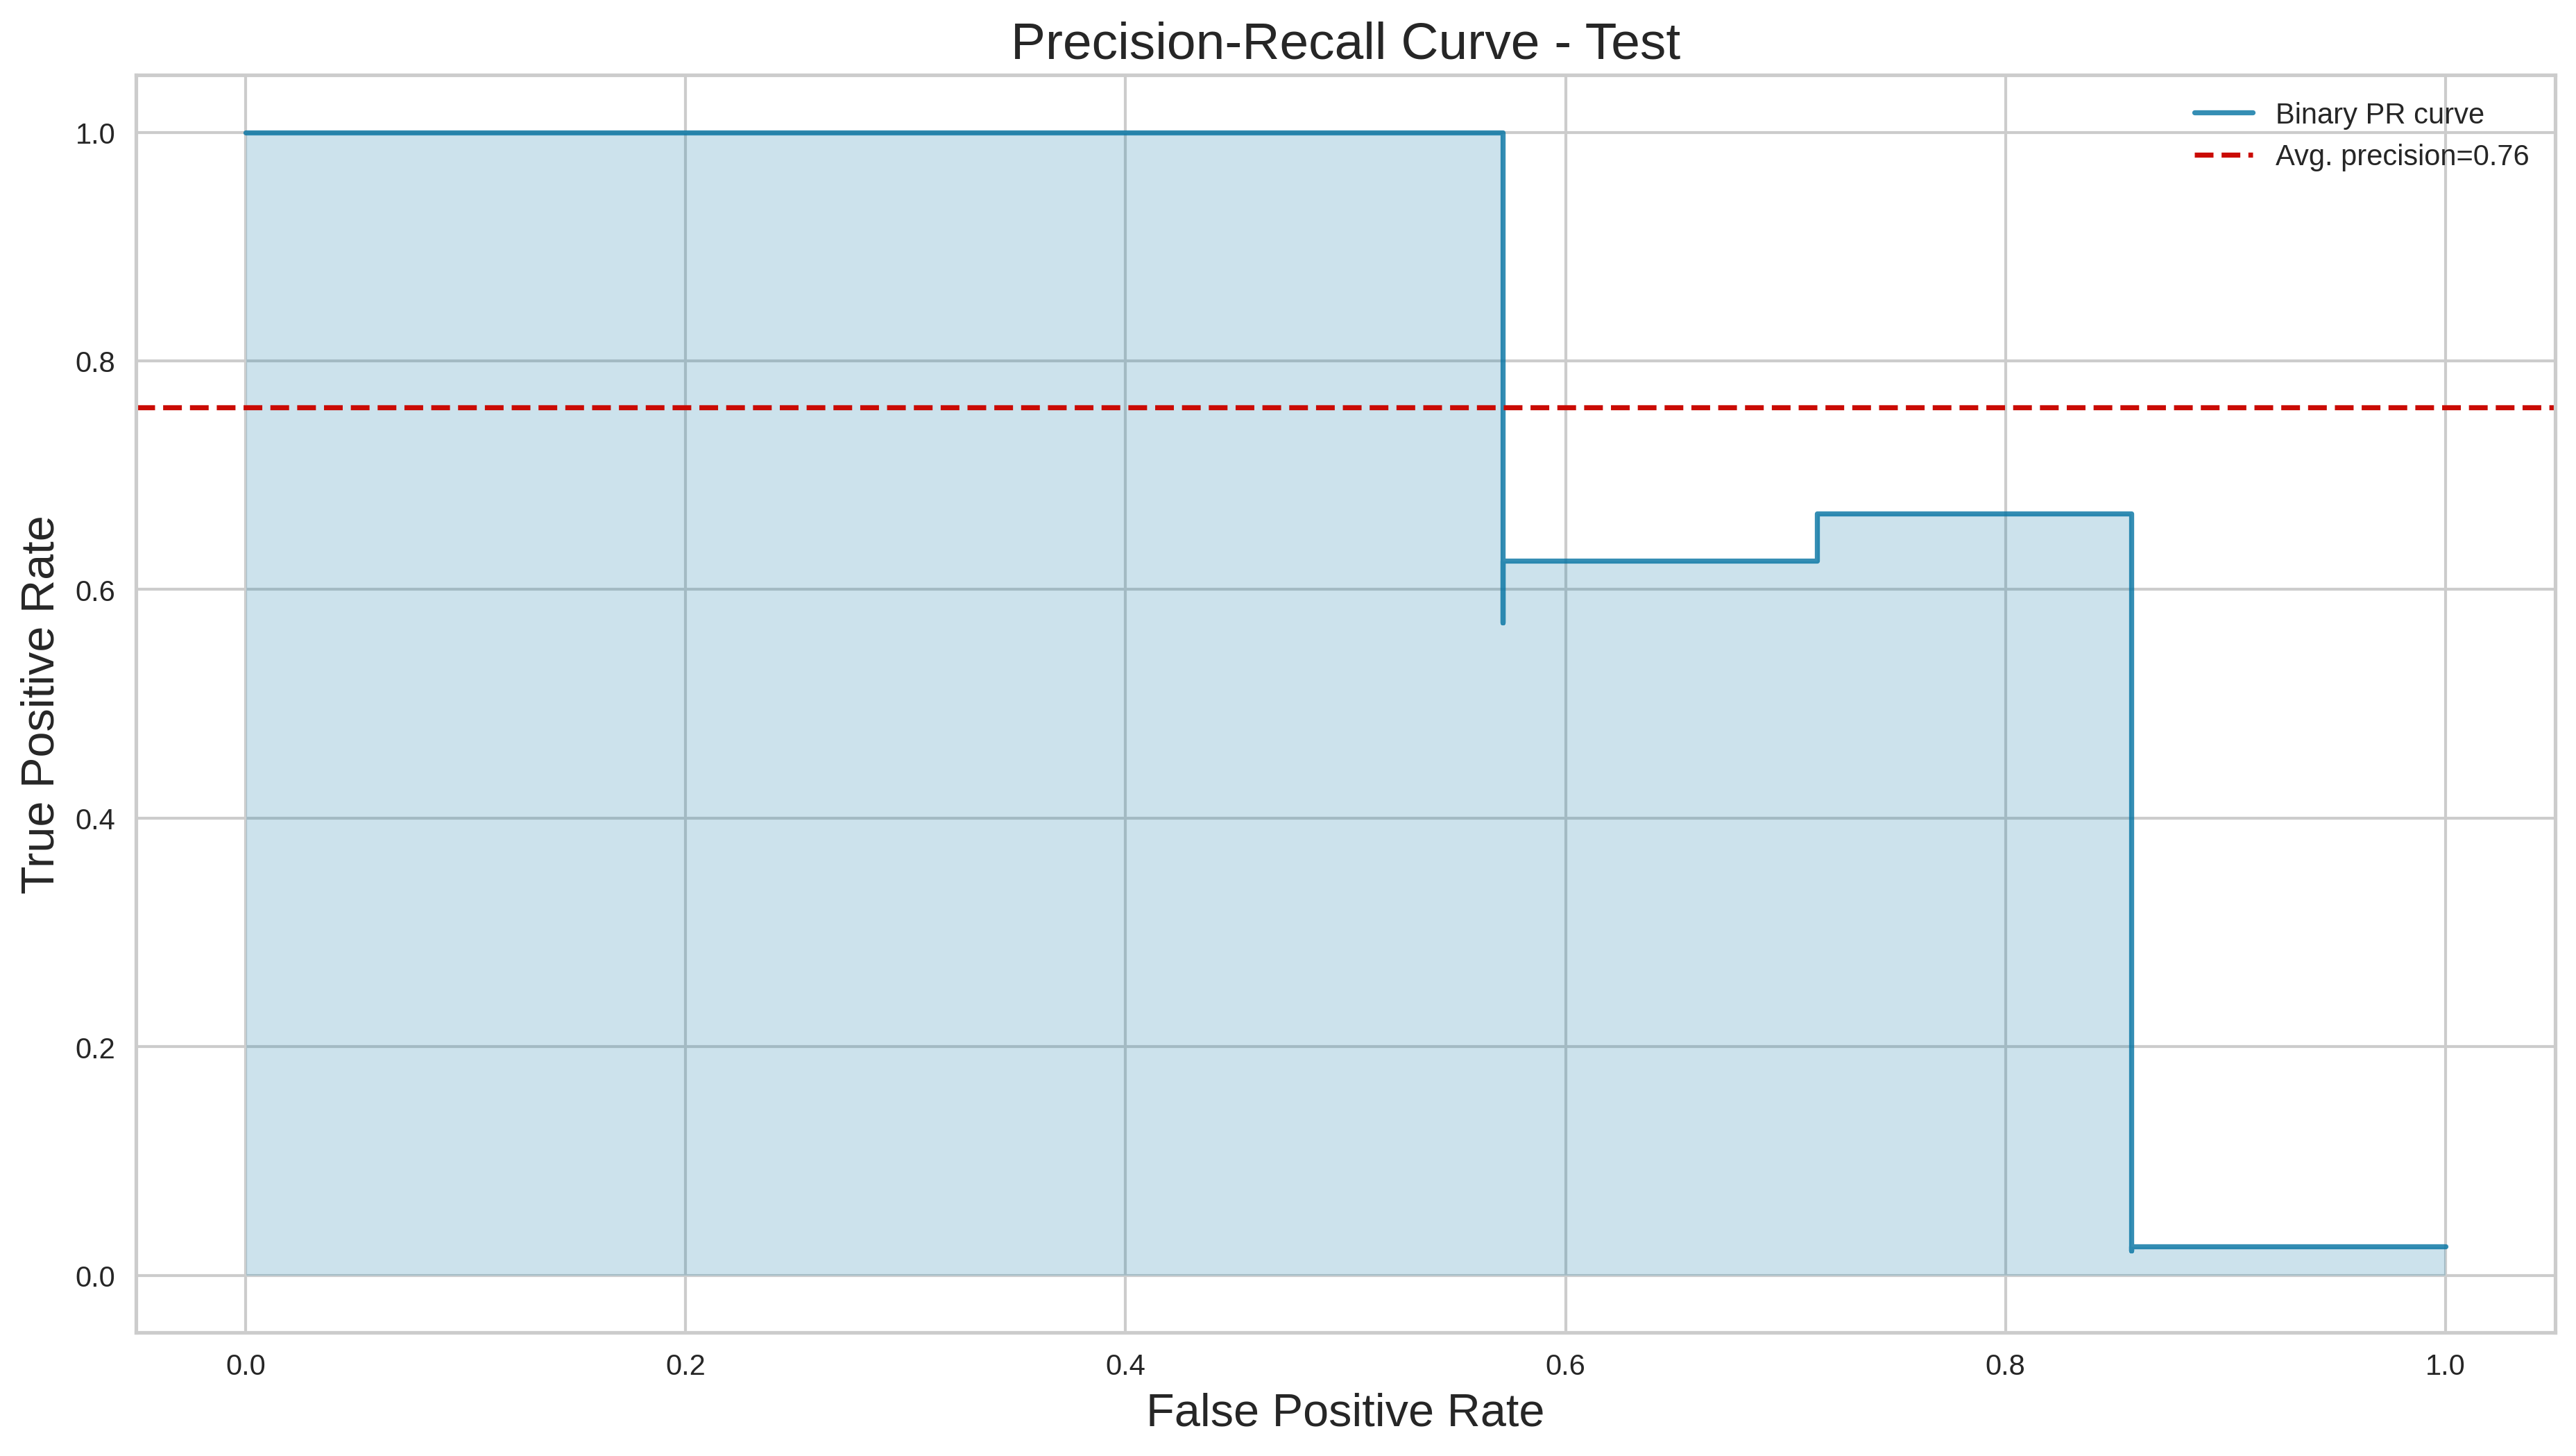
\includegraphics[width=16cm, keepaspectratio]{img/prec-rec-curve-test.png}
  \caption{Precision-Recall Curve corresponding to the results with the test dataset.}
  \label{fig:prec-rec-test}
\end{figure}

\begin{figure}
 \centering
  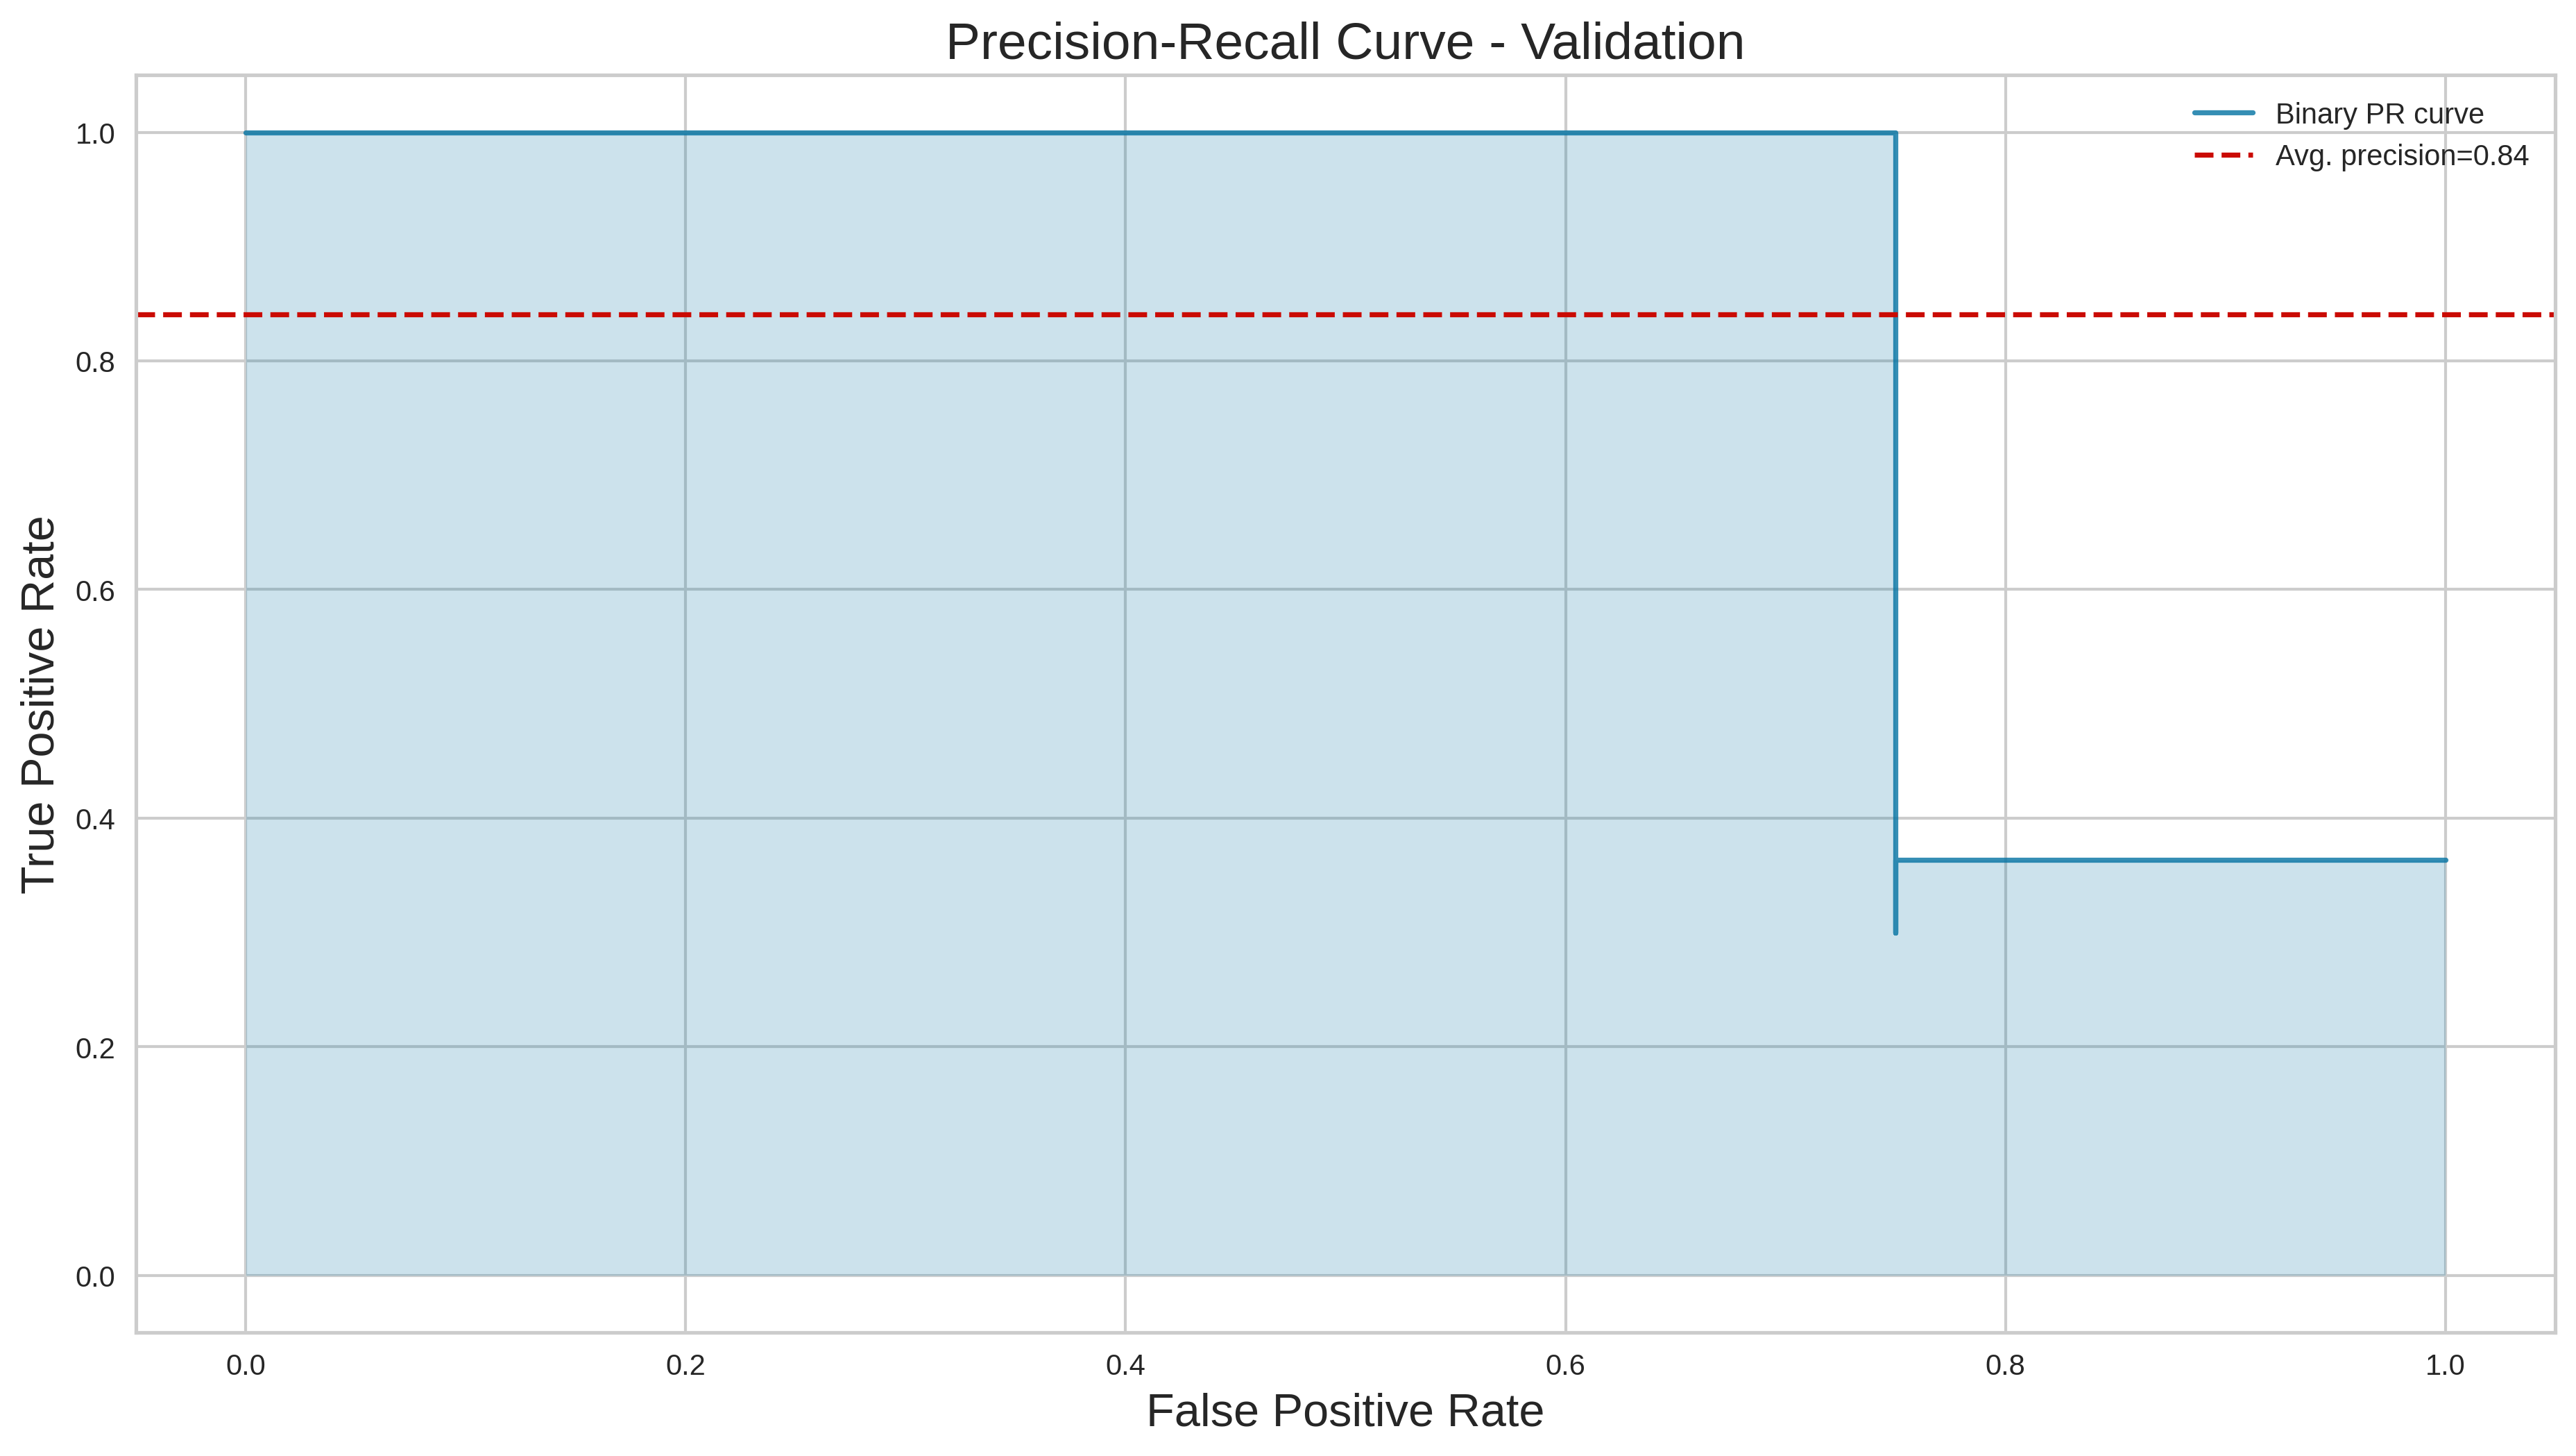
\includegraphics[width=16cm, keepaspectratio]{img/prec-rec-curve-val.png}
  \caption{Precision-Recall Curve corresponding to the results with the validation dataset.}
  \label{fig:prec-rec-val}
\end{figure}

\begin{figure}
 \centering
  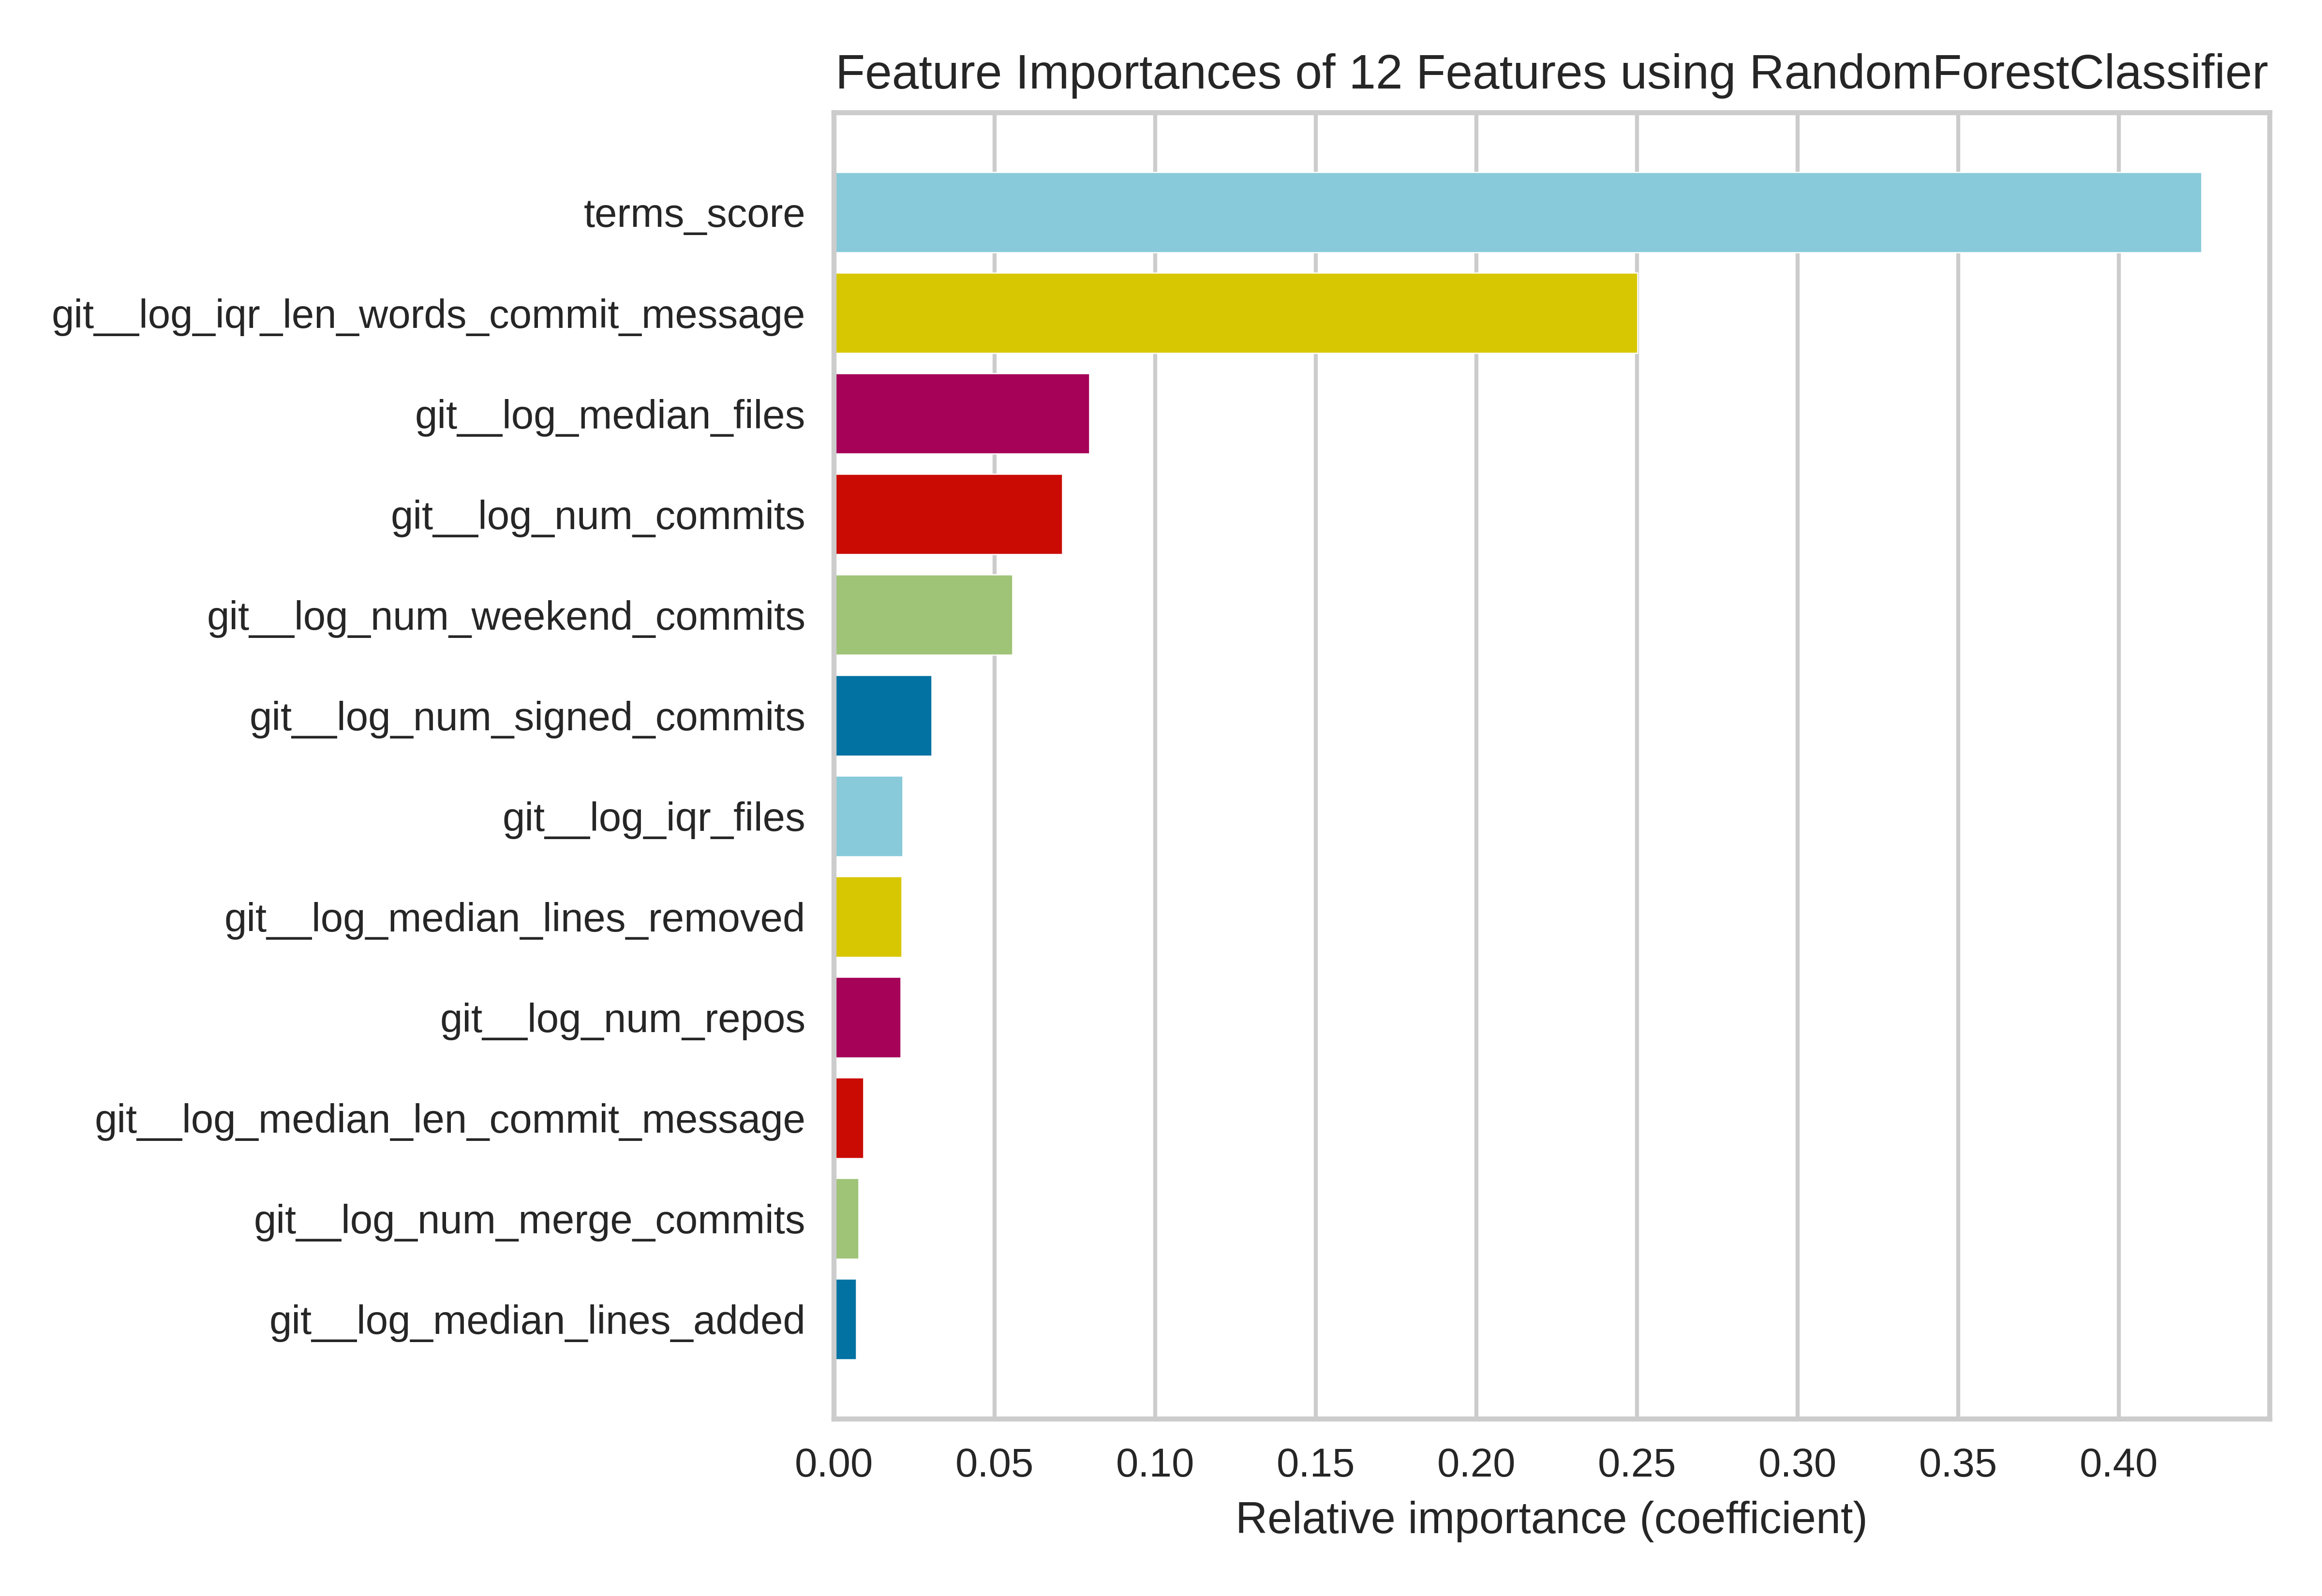
\includegraphics[width=16cm, keepaspectratio]{img/rf-feature-importances.png}
  \caption{Feature importance for the Random Forest Classifier, displayed in descending order.}
  \label{fig:rf-feature-importance}
\end{figure}


% \section{Inclusion of code}

% Es bastante habitual que se reproduzcan fragmentos de código en la memoria de un TFG/TFM.
% Esto permite explicar detalladamente partes del desarrollo que se ha realizado que se consideren
% de especial interés. No obstante, tampoco es conveniente pasarse e incluir demasiado código en
% la memoria, puesto que se puede alargar mucho el documento. Un recurso muy habitual es subir
% todo el código a un repositorio de un servicio de control de versiones como GitHub o GitLab,
% y luego incluir en la memoria la URL que enlace a dicho repositorio.

% Para incluir fragmentos de código en un documento \LaTeX se pueden combinar varias
% herramientas:

% \begin{itemize}
%     \item El entorno \mintinline{latex}{\begin{listing}[]...\end{listing}} permite crear
%     un marco en el que situar el fragmento de código (parecido al generado cuando insertamos
%     una tabla o una figura). Podemos insertar también una descripción (\textit{caption})
%     y una etiqueta para referenciarlo luego en el texto.
    
%     \item Dentro de este entorno, se puede utilizar el paquete 
%     \mintinline{latex}{minted}~\footnote{\url{https://es.overleaf.com/learn/latex/Code_Highlighting_with_minted}},
%     que utiliza el paquete Python Pygments para resaltado de sintaxis (coloreando el
%     código). Como se puede ver en el siguiente ejemplo, hay muchas opciones de configuración
%     que permiten controlar cómo se va a mostrar el código (incluir números de línea, saltos
%     de línea, tamaño y tipo de fuente, espaciado, código de colores para resaltado, etc.).
% \end{itemize}

% \begin{listing}[h!]
%     \caption{Lectura de un fichero *.csv y tipado de datos.}{}
%     \label{lst:1}
%     \begin{minted}[breaklines, fontsize=\footnotesize, baselinestretch=1]{python}
% # A dictionary is built to define the data type contained by each column
% dtype_scheme ={'budget': np.int64, 'genres': np.object, 'homepage': np.str, 'id': np.int64, 'keywords': np.object, 'original_language': np.str, 'original_title': np.str, 'overview': np.str, 'popularity': np.float64, 'production_companies': np.object, 'production_countries': np.object, 'release_date': np.object, 'revenue': np.int64, 'runtime': np.float64, 'spoken_languages': np.object,  'status': np.object, 'tagline': np.str, 'title': np.str, 'vote_average': np.float64, 'vote_count': np.int64}

% # When loading the data from the .csv file, we provide the scheme to be followed for data typing
% df1 = dd.read_csv('tmdb_5000_movies.csv', dtype=dtype_scheme)
%     \end{minted}
% \end{listing}

% Otra ventaja del entorno \verb|listing| es que se puede generar automáticamente un índice
% (con entradas hiperenlazadas) de fragmentos de código, para incluirlo al comienzo del 
% documento junto con los índices de figuras, tablas, etc.

% \subsection{Fuentes monoespaciadas}

% A veces se incluyen nombres de archivos, paquetes, etc. como texto monoespaciado, utilizando
% el comando \LaTeX \mintinline{latex}{\texttt{}}. Sin embargo, esto puede generar un problema
% cuando las palabras en fuente monoespaciada alcanzan el final de una línea. En ese caso,
% el compilador rehusa muchas veces romper la palabra y deja la línea demasiado larga respecto
% al resto.

% Para evitar esto, especialmente en párrafos más cortos de lo habitual (como en una lista
% no numerada), se puede utilizar el comando \mintinline{latex}{\begin{sloppypar}...\end{sloppypar}},
% como se muestra a continuación con un ejemplo real.
    
% \begin{itemize}
    
%     \begin{sloppypar} % Arregla longitud de línea en párrafos con fuente monoespaciada
%     \item Los valores contenidos en las columnas \texttt{genres}, \texttt{spoken\_languages}, \texttt{production\_companies} y \texttt{production\_countries}, clasificados originalmente como \texttt{np.objects}, se corresponden en realidad con listas de objetos \gls{json} que han sido almacenadas como cadenas de caracteres. A través de la función \texttt{get\_values(obj, key)} definida específicamente para ello, se transformará dicha cadena de caracteres en una lista de diccionarios a través de la función \texttt{json.loads(obj)} y se devolverá una  tupla que recopile los valores de los mismos para la clave indicada, un objeto de Python mucho más manejable de cara a realizar consultas sobre el \textit{dataset}.
%     \end{sloppypar}
    
% \end{itemize}

\cleardoublepage

%%%%%%%%%%%%%%%%%%%%%%%%%%%%%%%%%%%%%%%%%%%%%%%%%%%%%%%%%%%%%%%%%%%%%%%%%%%%%%%%
%%%%%%%%%%%%%%%%%%%%%%%%%%%%%%%%%%%%%%%%%%%%%%%%%%%%%%%%%%%%%%%%%%%%%%%%%%%%%%%%
% CONCLUSIONES %
%%%%%%%%%%%%%%%%%%%%%%%%%%%%%%%%%%%%%%%%%%%%%%%%%%%%%%%%%%%%%%%%%%%%%%%%%%%%%%%%


\chapter{Conclusions}
\label{chap:conclusions}

In this chapter, we recap the outcomes, achievements, and limitations of this project, after the objectives described in Section~\ref{sec:objectives}.

This project has been a long and complicated run. Although the main idea for the project was clear, the nature of the target problem implied a huge variety of problems and challenges. Likewise, the project development was affected by a global pandemic, which delayed and hinder its completion. Despite having faced many setbacks and limitations along the process, it is safe to say we are now able to provide answers to our initial objectives and also, enlighten the road for future work on this matter. Some of our hypotheses could not be bested, and some solutions did not work; but on the other hand, we found new research lines and solutions to explore in the future, gaining very valuable knowledge and experience along the journey.

\section{Goal achievements}
\label{sec:goal-achievements}

Regarding \textbf{Goal 1}, we can say we have achieved a well-defined process, including a classification model that works with the data obtained from the GrimoireLab toolset that allows us to discriminate between human users and bot accounts with reasonable accuracy. Due to the complexity of this project, the full automation and the integration was decided to be part of the future work (This links to the response to \textbf{Q1.4.}, available in subsection~\ref{ssec:integration-sortinghat}).

About the questions \textbf{Q1.1. }to \textbf{Q1.3.}: according to the results from the experiments, bot accounts can be separated from human users primarily by computing a score based on the terms included in their profile information and also computing a metric about the interquartile range of the number of words in the commit messages for a given individual, among other less-relevant features. Although the profile information from that individual is crucial for performing the classification, we can say it is not enough, and we need more features from the activity. The differences between this activity generated by humans and bots exist based on our observations, but we were not able to capture them in highly-relevant features for our classification model. Furthermore, we performed an experiment where the features were divided into two different subsets: one subset included the variables obtained from the activity, and the other the ones from the profile information. Then, the output from both classifiers was submitted to a voting classifier, but the results were not promising.

Following with \textbf{Goal 2}, we can provide a partial answer to \textbf{Q2.1.}, as we only have obtained data from Git commits. The outcome could be complemented by analysing other channels and finding another set of footprints that can lead to better results, also categorised as future work to improve this project.

To answer \textbf{Q2.2.}, we have observed that indeed the message content (such as the commit messages) is relevant to perform this classification, but more experiments would need to be run exploring more what we started at the experiment detailed in Section~\ref{sec:exp-text-richness} to give a more meaningful answer. Furthermore, to answer \textbf{Q2.3.}, we have observed that some of the activity details helped, such as the median number of files modified in each commit and the number of commits submitted during weekends, but their relevance was minor compared to the features detailed in the last section.

Last but not least, considering the \textbf{Goal 3}, we can safely say we have achieved a curated dataset from a real open-source community, in this case, Git commits from projects belonging to the Wikimedia Foundation (\textbf{Q3.1.}, \textbf{Q3.2.}). The curation of the identity information from the data we obtained was a hard, time-consuming task -even after having bot accounts identified by the community-, as all the unique identities were reviewed manually to get a dataset as accurate as possible. This process included cases that included mixed accounts, as they belonged to a human but also had submitted automated contributions using scripts or other processes. These cases, among others, would fit more in-depth research and another line of work for our classification tool.

% Esta sección es la sección espejo de las dos primeras del capítulo de objetivos, donde se planteaba el objetivo general y se elaboraban los específicos.

% Es aquí donde hay que debatir qué se ha conseguido y qué no. 
% Cuando algo no se ha conseguido, se ha de justificar, en términos de qué problemas se han encontrado y qué medidas se han tomado para mitigar esos problemas.

% Y si has llegado hasta aquí, siempre es bueno pasarle el corrector ortográfico, que las erratas quedan fatal en la memoria final.
% Para eso, en Linux tenemos aspell, que se ejecuta de la siguiente manera desde la línea de \emph{shell}:

% \begin{minted}{bash}
%   aspell --lang=es_ES -c memoria.tex
% \end{minted}

\section{Knowledge application}
\label{sec:knowledge-application}

Throughout this master's degree, I have acquired knowledge of important concepts and tools through various courses and developed the ability to tackle new challenges and apply my knowledge in different scenarios.

Specifically, these were the most relevant courses for this project:
\begin{enumerate}
\item \textbf{Fundamentos de Análisis de Datos} (Fundamentals of Data Analysis): This introductory course provided me with the context of the cycle of Data Science and the process behind a complete analysis.
\item \textbf{Machine Learning I} and \textbf{II}: These courses were especially valuable because their contents focus on classification and prediction models and a variety of techniques used along the process.
\item \textbf{Programación Orientada a Ciencia de Datos} (Data Science-oriented Programming): This course gave me the opportunity to gain more experience and knowledge to deal with the Data Science-related Python modules and tools.
\item \textbf{Text Mining}: In this course, I discovered a new field to explore, with concepts and techniques necessary for natural language.
\end{enumerate}

\section{Lessons learned}
\label{sec:lessons-learned}
% Aquí viene lo que has aprendido en el Trabajo Fin de Grado/Máster.

These are some of the learning outcomes I have reached thanks to this project:

\begin{enumerate}
  \item Consolidate and amplify the knowledge I obtained during the Master's courses, after applying a real-life use case and facing a variety of problems along the process.
  \item Foster my abilities in dealing with the programming side of data exploration and analysis, including new modules and techniques.
  \item A valuable perspective about the research process, with its peaks and valleys, finding new lines of work and new opportunities, even when the initial results are not good.
\end{enumerate}

\section{Future work}
\label{sec:future-work}

The complexity of this project increased unexpectedly due to the nature of the problem we aimed to solve. This left several questions unanswered, pending work and many research lines to be explored in order to improve the classification results and applicability of this tool.

\subsection{Improving and extending the classifier}

\textbf{Question:} Does this classifier work with the data from other open-source communities and other projects using bot accounts?

\begin{itemize}
    \item Once the classifier is trained for a given open-source project, is the result valid for other projects from the same community? And what about other communities?
\end{itemize}

To answer this question, we would need to test the current trained model with a different dataset. Also, this would help to answer if the obtained results are valid for other software projects and open-source communities or if there is a structured process that can be followed to adjust a set of parameters and improve the classifier's performance. For instance, one idea could be to include the heuristic terms in an external configuration file and categorise them in the three levels that were proposed. This list of terms could be adapted according to the project's needs and context.

\textbf{Question:} Are there other footprints that are helpful for this classification?

First, there could be a better way to build the initial dataset from the individual commits by finding other methods to summarise the information from the contributions of each individual. We also tried to separate the input features into two different categories: the ones coming from the activity and the ones coming from the individual's profile. The idea was to use separate classification models and choose the best result using a Voting classifier, but the results were not good.

Some of the strongest lines of future work are:
\begin{itemize}
    \item Keep studying the commit messages: We could not finish the experiment with the text distances. This and other related features and processes could help to improve this classifier.
    \item To augment this model by using the features from other data sources supported by GrimoireLab tools, such as GitHub Issues, Pull Requests and Comments. 
    \item Explore ``Concept Learning''~\cite{machinelearning-artdatascience} techniques to build the summarised information from all the contributions of a given individual and update the dataset incrementally (the more contributions an individual makes over time, the more information can be obtained from it).
    \item Mixed accounts (i.e., humans using automated tools) need to be studied more deeply. The classification would not be binary anymore but multi-class, leading to the possibility of characterising these automatic accounts using a smaller level of granularity. 
\end{itemize}

\subsection{Integration with SortingHat}
\label{ssec:integration-sortinghat}

This integration with GrimoireLab's identity management system was part of the initial design of the tool's architecture, but we decided to take this part out of the project's main scope.

In order to get \emph{Revelio} working with SortingHat, the trained model would need to be exported, and the classification results should be turned into a formatted report, including the identities potentially identified as bots and an accuracy score. This output would be used for SortingHat's recommendation engine, which produces a list of recommendations, in this case, a list of individual profiles that might get labelled as bots: The recommendations would be returned in ``Recommendation-like'' objects, referencing the individual, if it was classified as a bot, and an accuracy value from $0$ to $100$ (see Listing~\ref{lst:sh-recommend}). Also, unit and integration tests must be taken into account.

\begin{listing}[h!]
    \caption{Proposed class for SortingHat's recommendation engine to include the results of the classification.}{}
    \label{lst:sh-recommend}
    \begin{minted}[breaklines, fontsize=\footnotesize, baselinestretch=1]{python}
    class BotRecommendation(EntityBase):
        individual = ForeignKey(Individual, on_delete=CASCADE)
        is_bot = BooleanField(default=False)
        accuracy = PositiveIntegerField()

    class Meta:
        db_table = 'bot_recommendations'
        unique_together = ('individual',)

    def __str__(self):
        return '%s - %s - %s' % (self.individual, self.is_bot, self.accuracy)
    \end{minted}
\end{listing}


% Ningún proyecto ni software se termina, así que aquí vienen ideas y funcionalidades que estaría bien tener implementadas en el futuro.

% Es un apartado que sirve para dar ideas de cara a futuros TFGs/TFMs.

%%%%%%%%%%%%%%%%%%%%%%%%%%%%%%%%%%%%%%%%%%%%%%%%%%%%%%%%%%%%%%%%%%%%%%%%%%%%%%%%
%%%%%%%%%%%%%%%%%%%%%%%%%%%%%%%%%%%%%%%%%%%%%%%%%%%%%%%%%%%%%%%%%%%%%%%%%%%%%%%%
%%%%%%%%%%%%%%%%%%%%%%%%%%%%%%%%%%%%%%%%%%%%%%%%%%%%%%%%%%%%%%%%%%%%%%%%%%%%%%%%
% APPENDIX %
%%%%%%%%%%%%%%%%%%%%%%%%%%%%%%%%%%%%%%%%%%%%%%%%%%%%%%%%%%%%%%%%%%%%%%%%%%%%%%%%
\cleardoublepage
\appendix
%%%%%%%%%%%%%%%%%%%%%%%%%%%%%%%%%%%%%%%%%%%%%%%%%%%%%%%%%%%%%%%%%%%%%%%%%%%%%%%%
%%%%%%%%%%%%%%%%%%%%%%%%%%%%%%%%%%%%%%%%%%%%%%%%%%%%%%%%%%%%%%%%%%%%%%%%%%%%%%%%

\chapter{Definitions}
\label{app:app-definitions}

\section{Shifted logarithm}
\label{sec:form-one-plus-log10}

The decimal logarithm is shifted by $1$ to cover variables containing zero values.

\begin{center}
    \begin{equation}
        \mathrm{sLog_{10}}(x) = Log_{10}(1 + x) \quad .
    \end{equation}
\end{center}

\section{Jaccard distance}
\label{sec:jaccard-definition}

The Jaccard distance $J(c_{1}, c_{2})$ measures the distance between two character sequences $c_{1}$ and $c_{2}$ by comparing the number of distinct common words in $c_{1}$ and $c_{2}$ with the total number of distinct words in $c_{1}$ and $c_{2}$. 

\begin{center}
    \begin{equation}
    \mathrm{J}(c_{1}, c_{2}) = 1 - \frac{\left | words(c_{1})\bigcap words(c_{2}) \right | }{\left | words(c_{1})\bigcup words(c_{2}) \right | } \quad .
    \end{equation}
\end{center}

\section{Levenshtein distance}
\label{sec:levenshtein-definition}

The Levenshtein distance $Lev(c_{1}, c_{2})$ measures the difference between two character sequences $c_{1}$ and $c_{2}$ by counting the minimum number of single-character edits (insertion, deletion, or substitution) required to convert $c_{1}$ into $c_{2}$. The normalised version is computed as: 

\begin{center}
    \begin{equation}
        \mathrm{L}(c_{1}, c_{2}) = \frac{\textit{Lev}(c_{1}, c_{2})}{\textit{max}(\left | c_{1} \right |, \left | c_{2} \right | )} \quad .
    \end{equation}
\end{center}

\section{Combination of Jaccard and Levenshtein distances}
\label{sec:jacc-lev-comb-definition}

The combination of the Levenshtein and Jaccard distances from Mehdi et al. article is defined as follows:

\begin{center}
    \begin{equation}
        \mathrm{D}(c_{1}, c_{2}) = \frac{\textit{L}(c_{1}, c_{2}) + \textit{J}(c_{1}, c_{2})}{2} \quad ,
    \end{equation}
\end{center}

where $c_{1}$ and $c_{2}$ are two character sequences.

\section{Mahalanobis distance}
\label{sec:mahalanobis-definition}

The Mahalanobis distance is a measure of the distance between a point \(P\) and a distribution \(D\)~\cite{mclachlan1999mahalanobis}.

Given a probability distribution $Q$ on \(\mathbb{R} ^{N}\), with mean $\vec {\mu}=(\mu_{1},\mu_{2},\mu_{3}, \dots, \mu_{N})^{\mathsf {T}}$, and positive-definite covariance matrix $S$, the Mahalanobis distance of a point $\vec {x}=(x_{1},x_{2},x_{3},\dots ,x_{N})^{\mathsf {T}}$ from $Q$ is:

\begin{center}
    \begin{equation}
    d_{M}({\vec {x}},Q)={\sqrt {({\vec {x}}-{\vec {\mu }})^{\mathsf {T}}S^{-1}({\vec {x}}-{\vec {\mu }})}} \quad .
    \end{equation}
\end{center}

\section{Terms score}
\label{sec:terms-score-definition}

This terms score takes into account using different weighted heuristic terms, according to the knowledge domain. The terms are divided into $3$ different levels: terms from level $1$ have a weight of $60$, terms from level $2$ have a weight of $30$, and terms from level $3$ have a weight of $10$. 


The score is calculated as: 

\begin{center}
    \begin{equation}
        \mathrm {Ts}(term) = 60Nl_{1} + 30Nl_{2} + 10Nl_{3}\quad ,
    \end{equation}
\end{center}

where:
\begin{itemize}
    \item $Nl_{n}$ is the number of heuristics from level $n$ included in the term.
\end{itemize}

%%%%%%%%%%%%%%%%%%%%%%%%%%%%%%%%%%%%%%%%%%%%%%%%%%%%%%%%%%%%%%%%%%%%%%%%%%%%%%%%
% GLOSARIO(S) %
%%%%%%%%%%%%%%%%%%%%%%%%%%%%%%%%%%%%%%%%%%%%%%%%%%%%%%%%%%%%%%%%%%%%%%%%%%%%%%%%

\printglossary[type=\acronymtype]

\printglossary


%%%%%%%%%%%%%%%%%%%%%%%%%%%%%%%%%%%%%%%%%%%%%%%%%%%%%%%%%%%%%%%%%%%%%%%%%%%%%%%%
%%%%%%%%%%%%%%%%%%%%%%%%%%%%%%%%%%%%%%%%%%%%%%%%%%%%%%%%%%%%%%%%%%%%%%%%%%%%%%%%
% BIBLIOGRAFIA %
%%%%%%%%%%%%%%%%%%%%%%%%%%%%%%%%%%%%%%%%%%%%%%%%%%%%%%%%%%%%%%%%%%%%%%%%%%%%%%%%

\cleardoublepage

% https://www.overleaf.com/learn/latex/Bibliography_management_with_biblatex
\raggedright\printbibliography[heading=bibintoc,title={References}]

\end{document}
